%% For double-blind review submission, w/o CCS and ACM Reference (max submission space)
%\documentclass[acmsmall,review,anonymous]{acmart}\settopmatter{printfolios=true,printccs=false,printacmref=false}
%\documentclass[acmsmall]{acmart}\settopmatter{}
%% For editing double-blind review submission, w/o CCS and ACM Reference (max submission space)
\documentclass[acmsmall,screen]{acmart}\settopmatter{}
%% For double-blind review submission, w/ CCS and ACM Reference
%\documentclass[acmsmall,review,anonymous]{acmart}\settopmatter{printfolios=true}
%% For single-blind review submission, w/o CCS and ACM Reference (max submission space)
%\documentclass[acmsmall,review]{acmart}\settopmatter{printfolios=true,printccs=false,printacmref=false}
%% For single-blind review submission, w/ CCS and ACM Reference
%\documentclass[acmsmall,review]{acmart}\settopmatter{printfolios=true}
%% For final camera-ready submission, w/ required CCS and ACM Reference
%\documentclass[acmsmall]{acmart}\settopmatter{}

\begin{CCSXML}
<ccs2012>
<concept>
<concept_id>10002978.10002986.10002989</concept_id>
<concept_desc>Security and privacy~Formal security models</concept_desc>
<concept_significance>300</concept_significance>
</concept>
<concept>
<concept_id>10002978.10003006</concept_id>
<concept_desc>Security and privacy~Systems security</concept_desc>
<concept_significance>300</concept_significance>
</concept>
<concept>
<concept_id>10003752.10010124.10010138</concept_id>
<concept_desc>Theory of computation~Program reasoning</concept_desc>
<concept_significance>300</concept_significance>
</concept>
</ccs2012>
\end{CCSXML}

\ccsdesc[300]{Security and privacy~Formal security models}
\ccsdesc[300]{Security and privacy~Systems security}
\ccsdesc[300]{Theory of computation~Program reasoning}


%% Journal information
%% Supplied to authors by publisher for camera-ready submission;
%% use defaults for review submission.
% \acmJournal{PACMPL}
% \acmVolume{1}
% \acmNumber{CONF} % CONF = POPL or ICFP or OOPSLA
% \acmArticle{1}
% \acmYear{2018}
% \acmMonth{1}
% \acmDOI{} % \acmDOI{10.1145/nnnnnnn.nnnnnnn}
% \startPage{1}

%% Copyright information
%% Supplied to authors (based on authors' rights management selection;
%% see authors.acm.org) by publisher for camera-ready submission;
%% use 'none' for review submission.
% \setcopyright{none}
%\setcopyright{acmcopyright}
%\setcopyright{acmlicensed}
%\setcopyright{rightsretained}
%\copyrightyear{2018}           %% If different from \acmYear
\usepackage[utf8]{inputenc}

%% Bibliography style
\bibliographystyle{ACM-Reference-Format}
%% Citation style
%% Note: author/year citations are required for papers published as an
%% issue of PACMPL.
\citestyle{acmauthoryear}   %% For author/year citations


% %% Some recommended packages.
% \usepackage{booktabs}   %% For formal tables:
%                         %% http://ctan.org/pkg/booktabs
\usepackage{subcaption} %% For complex figures with subfigures/subcaptions
                        %% http://ctan.org/pkg/subcaption
\usepackage{wrapfig}

\usepackage{placeins}

\usepackage{todonotes}

\usepackage{ifthen}
\usepackage{pgf}
\usepackage{ulem}
\usepackage{tikz}
\usepackage{tikzpeople}
\usetikzlibrary{backgrounds}
\usetikzlibrary{fit}
\usetikzlibrary{calc}
\usetikzlibrary{positioning}
\usetikzlibrary{patterns}
\usetikzlibrary{decorations.pathreplacing}
\usetikzlibrary{arrows,shapes}
\usepackage{amssymb}

% Active adversary
\newcommand{\actadv}[4][]{
  \ifthenelse{\equal{#1}{}}{
    \draw[fill=white] #2 rectangle #3 node[pos=.5] {};
    \draw ($#2 + (2.25,1.5)$) node[devil,mirrored,minimum size=1cm] {};
    \draw[fill=white, fill opacity=0.5] #2 rectangle #3 node[pos=.5] {};
    \draw #2 rectangle #3 node[pos=.5,align=center] {\footnotesize #4};
  }{
    \onlyenv<#1>
    \draw[fill=white] #2 rectangle #3 node[pos=.5] {};
    \draw ($#2 + (3,1.5)$) node[devil,mirrored,minimum size=1cm] {};
    \draw[fill=white, fill opacity=0.5] #2 rectangle #3 node[pos=.5] {};
    \draw #2 rectangle #3 node[pos=.5,align=center] {\footnotesize #4};
    \endonlyenv
  }
}

% Inactive adversary
\newcommand{\inactadv}[4][]{
  \ifthenelse{\equal{#1}{}}{
    \draw[fill=white] #2 rectangle #3 node[pos=.5] {};
    \draw ($#2 + (2.25,1.5)$) node[devil,mirrored,minimum size=1cm] {};
    \draw[fill=white, fill opacity=0.4] #2 rectangle #3 node[pos=.5] {};
    \draw[fill=gray, fill opacity=0.5] #2 rectangle #3 node[pos=.5] {};
    \draw #2 rectangle #3 node[pos=.5,align=center] {\footnotesize #4};
  }{
    \onlyenv<#1>
    \draw[fill=white] #2 rectangle #3 node[pos=.5] {};
    \draw ($#2 + (3,1.5)$) node[devil,mirrored,minimum size=1cm] {};
    \draw[fill=white, fill opacity=0.4] #2 rectangle #3 node[pos=.5] {};
    \draw[fill=gray, fill opacity=0.5] #2 rectangle #3 node[pos=.5] {};
    \draw #2 rectangle #3 node[pos=.5,align=center] {\footnotesize #4};
    \endonlyenv
  }
}

% Active stack frame
\newcommand{\actsf}[4][]{
  \ifthenelse{\equal{#1}{}}{
    \draw[fill=white] #2 rectangle #3 node[pos=.5,align=center] {\footnotesize #4};
  }{
   \draw<#1>[fill=white] #2 rectangle #3 node[pos=.5,align=center] {#4};
 }
}

% Inactive stack frame
\newcommand{\inactsf}[4][]{
  \ifthenelse{\equal{#1}{}}{
    \draw[fill=white] #2 rectangle #3 node[pos=.5] {};
    \draw[fill=gray, fill opacity=0.5] #2 rectangle #3 node[pos=.5] {};
    \draw #2 rectangle #3 node[pos=.5,align=center] {\footnotesize #4};
  }{
    \draw<#1>[fill=white] #2 rectangle #3 node[pos=.5] {};
    \draw<#1>[fill=gray, fill opacity=0.5] #2 rectangle #3 node[pos=.5] {};
    \draw<#1> #2 rectangle #3 node[pos=.5,align=center] {\footnotesize #4};
  }
}

\newcommand{\capbrace}[4][sp1]{
  \draw [decorate,decoration={brace,amplitude=7pt,mirror,raise=4pt},yshift=0pt]
  #2 -- #3 node (#1) [black,midway,xshift=1cm,align=center] {\footnotesize #4};
}

\newcommand{\lincapbrace}[4][sp1]{
  \draw [densely dotted,decorate,decoration={brace,amplitude=7pt,mirror,raise=4pt},yshift=0pt]
  #2 -- #3 node (#1) [black,midway,xshift=1cm,align=center] {\footnotesize #4};
}

\newcommand{\capbracebot}[4][sp1]{
  \draw [decorate,decoration={brace,amplitude=7pt,mirror,raise=4pt,aspect=0.25},yshift=0pt]
  #2 -- #3 node (#1) [black,near start,xshift=1cm,align=center] {\footnotesize #4};
}

\newcommand{\lincapbracebot}[4][sp1]{
  \draw [densely dotted,decorate,decoration={brace,amplitude=7pt,mirror,raise=4pt,aspect=0.25},yshift=0pt]
  #2 -- #3 node (#1) [black,near start,xshift=1cm,align=center] {\footnotesize #4};
}


\newcommand{\capbracebotred}[4][sp1]{
  \draw [decorate,red,decoration={brace,amplitude=7pt,mirror,raise=4pt,aspect=0.25},yshift=0pt]
  #2 -- #3 node (#1) [red,near start,xshift=1cm,align=center] {\footnotesize #4};
}

\newcommand{\redcross}[2][1]{
  \draw ($#2 + (-#1/2,#1/2)$) edge[color=red,thick] ($#2 + (#1/2,-#1/2)$)
        ($#2 + (#1/2,#1/2)$) edge[color=red,thick] ($#2 + (-#1/2,-#1/2)$);
  
}


\newcommand{\stdstackstartclean}[1][11]{
  \scope
    \clip (-.1,-.1) rectangle (4.6,#1 + .1);
    \fill[fill=white] (0,0) rectangle (4.5,#1);
    \draw (0,0) -- (0,#1);
    \draw (4.5,0) -- (4.5,#1);
  \endscope
  % \draw[->] (-2,0) -- node[midway,sloped,above] {stack grows upward} (-2,15);
  \draw (-1.5,0) node {};
  \draw (-1.5,#1 + 1) node {};
}

\newcommand{\stdstackstart}[1][11]{
  \scope
    \clip (-.1,-.1) rectangle (4.6,#1 + .1);
    \fill[fill=white] (0,0) rectangle (4.5,#1);
    \draw (0,0) -- (0,#1);
    \draw (4.5,0) -- (4.5,#1);
    \draw[fill=gray!50] (0,-.5) rectangle (4.5,2)node[pos=.5,color=black,align=center,yshift=0.1cm] {\footnotesize Lower stack\\\footnotesize frames...};
  \endscope
  % \draw[->] (-2,0) -- node[midway,sloped,above] {stack grows upward} (-2,15);
  \draw (-1.5,0) node {};
  \draw (-1.5,#1 + 1) node {};
}

% stolen from https://tex.stackexchange.com/questions/14225/is-there-the-easiest-way-to-toggle-show-hide-navigational-grids-in-tikz/14230
\makeatletter
\newif\if@showgrid@grid
\newif\if@showgrid@left
\newif\if@showgrid@right
\newif\if@showgrid@below
\newif\if@showgrid@above
\tikzset{%
    every show grid/.style={},
    show grid/.style={execute at end picture={\@showgrid{grid=true,#1}}},%
    show grid/.default={true},
    show grid/.cd,
    labels/.style={font={\sffamily\small},help lines},
    xlabels/.style={},
    ylabels/.style={},
    keep bb/.code={\useasboundingbox (current bounding box.south west) rectangle (current bounding box.north west);},
    true/.style={left,below},
    false/.style={left=false,right=false,above=false,below=false,grid=false},
    none/.style={left=false,right=false,above=false,below=false},
    all/.style={left=true,right=true,above=true,below=true},
    grid/.is if=@showgrid@grid,
    left/.is if=@showgrid@left,
    right/.is if=@showgrid@right,
    below/.is if=@showgrid@below,
    above/.is if=@showgrid@above,
    false,
}

\def\@showgrid#1{%
    \begin{scope}[every show grid,show grid/.cd,#1]
    \if@showgrid@grid
    \begin{pgfonlayer}{background}
    \draw [help lines]
        (current bounding box.south west) grid
        (current bounding box.north east);
%
    \pgfpointxy{1}{1}%
    \edef\xs{\the\pgf@x}%
    \edef\ys{\the\pgf@y}%
    \pgfpointanchor{current bounding box}{south west}
    \edef\xa{\the\pgf@x}%
    \edef\ya{\the\pgf@y}%
    \pgfpointanchor{current bounding box}{north east}
    \edef\xb{\the\pgf@x}%
    \edef\yb{\the\pgf@y}%
    \pgfmathtruncatemacro\xbeg{ceil(\xa/\xs)}
    \pgfmathtruncatemacro\xend{floor(\xb/\xs)}
    \if@showgrid@below
    \foreach \X in {\xbeg,...,\xend} {
        \node [below,show grid/labels,show grid/xlabels] at (\X,\ya) {\X};
    }
    \fi
    \if@showgrid@above
    \foreach \X in {\xbeg,...,\xend} {
        \node [above,show grid/labels,show grid/xlabels] at (\X,\yb) {\X};
    }
    \fi
    \pgfmathtruncatemacro\ybeg{ceil(\ya/\ys)}
    \pgfmathtruncatemacro\yend{floor(\yb/\ys)}
    \if@showgrid@left
    \foreach \Y in {\ybeg,...,\yend} {
        \node [left,show grid/labels,show grid/ylabels] at (\xa,\Y) {\Y};
    }
    \fi
    \if@showgrid@right
    \foreach \Y in {\ybeg,...,\yend} {
        \node [right,show grid/labels,show grid/ylabels] at (\xb,\Y) {\Y};
    }
    \fi
    \end{pgfonlayer}
    \fi
    \end{scope}
}
\makeatother


 	
%%% Local Variables:
%%% TeX-master: "paper"
%%% End:
\usetikzlibrary{fit}
\makeatletter
\tikzset{
  fitting node/.style={
    inner sep=0pt,
    fill=none,
    draw=none,
    reset transform,
    fit={(\pgf@pathminx,\pgf@pathminy) (\pgf@pathmaxx,\pgf@pathmaxy)}
  },
  reset transform/.code={\pgftransformreset}
}
\makeatother

% Math packages
\usepackage{amsmath,amsfonts,amssymb,amsthm}
\usepackage{mathrsfs}
\usepackage{thmtools}
\usepackage{array}
\usepackage{cleveref}
\usepackage{stmaryrd}
\usepackage{mathpartir}


% Command control packages
\usepackage{ifthen}
\usepackage{ifpdf}

% Listings
\usepackage{listings}
\lstset{
  basicstyle=\ttfamily,
  columns=fullflexible,
  keepspaces=true,
  mathescape
}


% Tikz
\usepackage{tikz}

%%% Comments
% Comments
\newcommand\lau[1]{{\color{purple} \sf \footnotesize {LS: #1}}\\}
\newcommand\dominique[1]{{\color{purple} \sf \footnotesize {DD: #1}}\\}
\newcommand\lars[1]{{\color{purple} \sf \footnotesize {LB: #1}}\\}

%%% Math environments
\declaretheorem[numbered=yes,name=Lemma,qed=$\blacksquare$]{lemma}
\declaretheorem[numbered=yes,name=Theorem,qed=$\blacksquare$]{theorem}
\declaretheorem[numbered=yes,name=Definition,qed=$\blacksquare$]{definition}
\declaretheorem[numbered=yes,name=Specification,qed=$\blacksquare$]{specification}


%%% Math notation
\newcommand{\defeq}{\stackrel{\textit{\tiny{def}}}{=}}
\newcommand{\defbnf}{::=}
\newcommand{\sem}[1]{\left\llbracket #1 \right\rrbracket}
\newcommand{\ssem}[2][\Phi]{\sem{#2}_{\mathrm{src}}(#1)}
\newcommand{\tsem}[2][\Phi]{\sem{#2}_{\mathrm{trg}}(#1)}
\newcommand{\dom}{\mathrm{dom}}
\newcommand{\powerset}[1]{\mathcal{P}(#1)}

\newcommand{\npair}[2][n]{\left(#1,#2\right)}

\newcommand{\nsubeq}[1][n]{\overset{#1}{\subseteq}}
\newcommand{\nsupeq}[1][n]{\overset{#1}{\supseteq}}
\newcommand{\nequal}[1][n]{\overset{#1}{=}}

% Function arrows
\newcommand{\fun}{\rightarrow}
\newcommand{\parfun}{\rightharpoonup}
\newcommand{\monnefun}{\xrightarrow{\textit{\tiny{mon, ne}}}}



% Text
\newcommand{\tand}{\text{ and }}
\newcommand{\tor}{\text{ or }}
\newcommand{\totherwise}{\text{otherwise }}

% Equivalences
\newcommand{\sconeq}{\mathrel{\src{\approx_{\mathrm{ctx}}}}}
\newcommand{\tconeq}{\mathrel{\approx_{\mathrm{ctx}}}}

%%% Logical Relation notation
\newcommand{\typesetlr}[1]{\mathcal{#1}}
\newcommand{\lre}[1][\square]{\typesetlr{E}^{#1}}
\newcommand{\lrexj}[1][\square]{\typesetlr{E}^{#1}_{\var{xjmp}}}
\newcommand{\lrk}[1][\square]{\typesetlr{K}^{#1}}
\newcommand{\lrr}[1][\square]{\typesetlr{R}^{#1}}
\newcommand{\lro}[1][\square]{\typesetlr{O}^{#1}}
\newcommand{\lrol}{\lro[\preceq]}
\newcommand{\lror}{\lro[\succeq]}
\newcommand{\lrv}[1][\square]{\typesetlr{V}^{#1}}
\newcommand{\lrp}[1][\square]{\typesetlr{P}^{#1}}

\newcommand{\lrrs}{\typesetlr{R}}
\newcommand{\lrm}{\typesetlr{M}}

\newcommand{\stpair}[3][]{
\ifthenelse{\equal{#1}{}}
{\left(\src{#2_S},#3_T\right)}
{\left(\src{#2},#3\right)}}


\newcommand{\memSatGeneric}[4]{#2 :_{#1}^{#4}#3}
\newcommand{\memSat}[3][n]{\memSatGeneric{#1}{#2}{#3}{}}
\newcommand{\memSatStack}[3][n]{\memSatGeneric{#1}{#2}{#3}{\text{priv\_stack}}}
\newcommand{\memSatFStack}[3][n]{\memSatGeneric{#1}{#2}{#3}{\text{free\_stack}}}
\newcommand{\memSatHeap}[3][n]{\memSatGeneric{#1}{#2}{#3}{\text{heap}}}


\newcommand{\World}{\mathrm{World}}
\newcommand{\Worlds}{\mathrm{World}_\text{private stack}}
\newcommand{\Worldh}{\mathrm{World}_\mathrm{heap}}
\newcommand{\Worldfs}{\mathrm{World}_\text{free stack}}


\newcommand{\RegionName}{\mathrm{RegionName}}
\newcommand{\Region}{\mathrm{Region}}
\newcommand{\Regions}{\mathrm{Region}_\mathrm{spatial}}
\newcommand{\Regionh}{\mathrm{Region}_\mathrm{shared}}

\newcommand{\spatial}{\mathrm{spatial}}
\newcommand{\spatialo}{\mathrm{spatial\_owned}}
\newcommand{\pure}{\mathrm{pure}}
\newcommand{\revoked}{\mathrm{revoked}}

\newcommand{\State}{\mathrm{State}}
\newcommand{\Rels}{\mathrm{Rels}}
\newcommand{\UPred}[1]{\mathrm{UPred}(#1)}
\newcommand{\URel}[1]{\mathrm{URel}(#1)}

\newcommand{\future}{\sqsupseteq}
\newcommand{\pub}{\mathrm{pub}}
\newcommand{\privft}{\future^{\priv}}
\newcommand{\pubft}{\future^{\pub}}
% \newcommand{\monprivnefun}{\xrightarrow[\text{\tiny{$\privft$}}]{\textit{\tiny{mon, ne}}}}
% \newcommand{\monpubnefun}{\xrightarrow[\text{\tiny{$\pubft$}}]{\textit{\tiny{mon, ne}}}}

%%% Regions
\newcommand{\stdreg}[2]{\iota^{\mathrm{std},#2}_{#1}}
\newcommand{\stareg}[2][\stpair{\ms}{\ms}]{\iota^{\mathrm{sta},#2}_{#1}}
\newcommand{\staureg}[2][\stpair{\ms}{\ms}]{\iota^{\mathrm{sta,\lrv},#2}_{#1}}
\newcommand{\spa}{\mathrm{s}}
\newcommand{\spao}{\mathrm{so}}
\newcommand{\pur}{\mathrm{p}}

%%% Instruction formatting
\newcommand{\sourcecolortext}{blue}
\newcommand{\sourcecolor}{\color{blue}}
\newcommand{\src}[1]{{\sourcecolor #1}}
\newcommand{\targetcolortext}{black}
\newcommand{\targetcolor}[1]{\color{black}}
\newcommand{\trg}[1]{{\targetcolor{} #1}}

\newcommand{\zinstr}[1]{\texttt{#1}}
\newcommand{\oneinstr}[2]{
  \ifthenelse{\equal{#2}{}}
  {\zinstr{#1}}
  {\zinstr{#1} \; #2}
}
\newcommand{\twoinstr}[3]{
  \ifthenelse{\equal{#2#3}{}}
  {\zinstr{#1}}
  {\zinstr{#1} \; #2 \; #3}
}
\newcommand{\threeinstr}[4]{
  \ifthenelse{\equal{#2#3#4}{}}
  {\zinstr{#1}}
  {\zinstr{#1} \; #2 \; #3 \; #4}
}

\newcommand{\fourinstr}[5]{
  \ifthenelse{\equal{#2#3#4#5}{}}
  {\zinstr{#1}}
  {\zinstr{#1} \; #2 \; #3 \; #4 \; #5}
}


%%% Source language
% No arguments
\newcommand{\sfail}{\zinstr{\src{fail}}}
\newcommand{\shalt}{\zinstr{\src{halt}}}
\newcommand{\sreturn}{\zinstr{\src{return}}}

% One argument
\newcommand{\sjmp}[1]{\oneinstr{\src{jmp}}{#1}}
\newcommand{\spush}[1]{\oneinstr{\src{push}}{#1}}
\newcommand{\spop}[1]{\oneinstr{\src{pop}}{#1}}

% Two arguments
\newcommand{\sjnz}[2]{\twoinstr{\src{jnz}}{#1}{#2}}
\newcommand{\sisptr}[2]{\twoinstr{\src{gettype}}{#1}{#2}}
\newcommand{\sgeta}[2]{\twoinstr{\src{geta}}{#1}{#2}}
\newcommand{\sgetb}[2]{\twoinstr{\src{getb}}{#1}{#2}}
\newcommand{\sgete}[2]{\twoinstr{\src{gete}}{#1}{#2}}
\newcommand{\sgetp}[2]{\twoinstr{\src{getp}}{#1}{#2}}
%\newcommand{\sgetloc}[2]{\twoinstr{\src{getloc}}{#1}{#2}}
\newcommand{\sgetlin}[2]{\twoinstr{\src{get}}{#1}{#2}}
\newcommand{\smove}[2]{\twoinstr{\src{move}}{#1}{#2}}
\newcommand{\sstore}[2]{\twoinstr{\src{store}}{#1}{#2}}
\newcommand{\sload}[2]{\twoinstr{\src{load}}{#1}{#2}}
\newcommand{\scca}[2]{\twoinstr{\src{cca}}{#1}{#2}}
\newcommand{\ssload}[2]{\twoinstr{\src{sload}}{#1}{#2}}
\newcommand{\sxjmp}[2]{\twoinstr{\src{xjmp}}{#1}{#2}}
\newcommand{\ssetatob}[2]{\twoinstr{\src{seta2b}}{#1}{#2}}
% scall - special two instruction
\newcommand{\scall}[4][]{  
\ifthenelse{\equal{#3#4}{}}
  {\ensuremath{\zinstr{\src{call}}_{#1}^{#2}}}
  {\ensuremath{\zinstr{\src{call}}_{#1}^{#2} \; #3 \; #4}}
}


% Three arguments
\newcommand{\srestrict}[3]{\threeinstr{\src{restrict}}{#1}{#2}{#3}}
\newcommand{\slt}[3]{\threeinstr{\src{lt}}{#1}{#2}{#3}}
\newcommand{\splus}[3]{\threeinstr{\src{plus}}{#1}{#2}{#3}}
\newcommand{\sminus}[3]{\threeinstr{\src{minus}}{#1}{#2}{#3}}
\newcommand{\scseal}[3]{\threeinstr{\src{cseal}}{#1}{#2}{#3}}
\newcommand{\ssplice}[3]{\threeinstr{\src{splice}}{#1}{#2}{#3}}

% 
% Four arguments
%\newcommand{\ssubseg}[4]{\fourinstr{\src{subseg}}{#1}{#2}{#3}{#4}}
\newcommand{\ssplit}[4]{\fourinstr{\src{split}}{#1}{#2}{#3}{#4}}

%%% Target language
% No arguments
\newcommand{\tfail}{\zinstr{\trg{fail}}}
\newcommand{\thalt}{\zinstr{\trg{halt}}}

% One argument
\newcommand{\tjmp}[1]{\oneinstr{\trg{jmp}}{#1}}
\newcommand{\tsetatob}[1]{\oneinstr{\trg{seta2b}}{#1}}

% Two arguments
\newcommand{\tjnz}[2]{\twoinstr{\trg{jnz}}{#1}{#2}}
\newcommand{\tisptr}[2]{\twoinstr{\trg{gettype}}{#1}{#2}}
\newcommand{\tgeta}[2]{\twoinstr{\trg{geta}}{#1}{#2}}
\newcommand{\tgetb}[2]{\twoinstr{\trg{getb}}{#1}{#2}}
\newcommand{\tgete}[2]{\twoinstr{\trg{gete}}{#1}{#2}}
\newcommand{\tgetp}[2]{\twoinstr{\trg{getp}}{#1}{#2}}
%\newcommand{\tgetloc}[2]{\twoinstr{\trg{getloc}}{#1}{#2}}
\newcommand{\tgetlin}[2]{\twoinstr{\trg{getl}}{#1}{#2}}
\newcommand{\tmove}[2]{\twoinstr{\trg{move}}{#1}{#2}}
\newcommand{\tstore}[2]{\twoinstr{\trg{store}}{#1}{#2}}
\newcommand{\tload}[2]{\twoinstr{\trg{load}}{#1}{#2}}
\newcommand{\tcca}[2]{\twoinstr{\trg{cca}}{#1}{#2}}
\newcommand{\txjmp}[2]{\twoinstr{\trg{xjmp}}{#1}{#2}}
\newcommand{\trestrict}[2]{\twoinstr{\trg{restrict}}{#1}{#2}}

% Three arguments
\newcommand{\tsplice}[3]{\threeinstr{\trg{splice}}{#1}{#2}{#3}}
\newcommand{\tlt}[3]{\threeinstr{\trg{lt}}{#1}{#2}{#3}}
\newcommand{\tplus}[3]{\threeinstr{\trg{plus}}{#1}{#2}{#3}}
\newcommand{\tminus}[3]{\threeinstr{\trg{minus}}{#1}{#2}{#3}}
\newcommand{\tcseal}[3]{\threeinstr{\trg{cseal}}{#1}{#2}{#3}}

% Four arguments
%\newcommand{\tsubseg}[4]{\fourinstr{\trg{subseg}}{#1}{#2}{#3}{#4}}
\newcommand{\tsplit}[4]{\fourinstr{\trg{split}}{#1}{#2}{#3}{#4}}

%%% Domains
\newcommand{\plaindom}[1]{\mathrm{#1}}

\newcommand{\nats}{\mathbb{N}}
\newcommand{\ints}{\mathbb{Z}}

\newcommand{\ta}{T_A}

%%% Updates
\newcommand{\update}[2]{[#1 \mapsto #2]}
\newcommand{\updReg}[2]{\update{\reg.#1}{#2}}
\newcommand{\updPc}[1]{\Phi\updReg{\pcreg}{#1}}

%%% Source dom
\newcommand{\shareddom}[1]{\mathrm{#1}}
\newcommand{\RegName}{\shareddom{RegisterName}}
\newcommand{\Addr}{\shareddom{Addr}}
\newcommand{\Seal}{\shareddom{Seal}}
\newcommand{\Perm}{\shareddom{Perm}}
\newcommand{\Caps}{\shareddom{Cap}}
\newcommand{\SealableCaps}{\shareddom{SealableCap}}
\newcommand{\Word}{\shareddom{Word}}
\newcommand{\Instr}{\shareddom{Instr}}
\newcommand{\Mem}{\shareddom{Memory}}
\newcommand{\Reg}{\shareddom{RegisterFile}}
\newcommand{\Stk}{\shareddom{Stack}}
\newcommand{\Conf}{\shareddom{Conf}}
\newcommand{\ExecConf}{\shareddom{ExecConf}}
%\newcommand{\Global}{\shareddom{Global}}
\newcommand{\Linear}{\shareddom{Linear}}
\newcommand{\MemSeg}{\shareddom{MemorySegment}}
\newcommand{\StkFrame}{\shareddom{StackFrame}}
\newcommand{\Stack}{\shareddom{Stack}}

\newcommand{\scbnf}{\shareddom{sc}}
\newcommand{\cbnf}{\shareddom{c}}
\newcommand{\permbnf}{\shareddom{perm}}
\newcommand{\addrbnf}{\shareddom{a}}
\newcommand{\basebnf}{\shareddom{base}}
\newcommand{\aendbnf}{\shareddom{end}}
\newcommand{\rbnf}{\shareddom{r}}
%\newcommand{\glbnf}{\shareddom{gl}}
\newcommand{\linbnf}{\shareddom{l}}
\newcommand{\sealbasebnf}{\sigma_\shareddom{base}}
\newcommand{\sealendbnf}{\sigma_\shareddom{end}}

\newcommand{\sstk}{\shareddom{stk}}
\newcommand{\smsstk}{\shareddom{ms_{stk}}}
\newcommand{\sstkframe}{\shareddom{frame}}
\newcommand{\sopc}{\shareddom{opc}}
\newcommand{\sastk}{\shareddom{a_{stk}}}
\newcommand{\perm}{\var{perm}}
%\newcommand{\gl}{\var{g}}
\newcommand{\lin}{\var{l}}
\newcommand{\base}{\shareddom{base}}
\newcommand{\aend}{\shareddom{end}}
\newcommand{\addr}{\shareddom{a}}
\newcommand{\scap}{\shareddom{c}}
\newcommand{\sms}{\shareddom{ms}}

\newcommand{\stkptr}[1]{\mathrm{stack\text{-}ptr}(#1)}
\newcommand{\retptr}{\mathrm{ret\text{-}ptr}}
\newcommand{\retptrd}{\mathrm{ret\text{-}ptr\text{-}data}}
\newcommand{\retptrc}{\mathrm{ret\text{-}ptr\text{-}code}}

\newcommand{\seal}[1]{\shareddom{seal}(#1)}
\newcommand{\sealed}[1]{\shareddom{sealed}(#1)}

\newcommand{\failed}{\mathrm{failed}}
% DOMI: defining a macro named ``undefined'' breaks many latex packages.
%       (this is just another way that LaTeX is broken as a programming language)
% \newcommand{\undefined}{\mathrm{undefined}}
\newcommand{\tundefined}{\mathrm{undefined}}
\newcommand{\halted}{\mathrm{halted}}

%%% Target domain
\newcommand{\targetdom}[1]{\mathrm{#1}}
\newcommand{\tRegName}{\targetdom{RegisterName}}

%%% Programs and contexts
\newcommand{\program}{\mathscr{P}}
\newcommand{\context}{\mathscr{C}}

\newcommand{\plug}[2]{#1[#2]}

%%% Operational semantics
\newcommand{\step}{\rightarrow}
\newcommand{\nstep}[1][n]{\step_{#1}}
\newcommand{\steps}{\step^*}
\newcommand{\diverge}{{\Uparrow}}
\newcommand{\term}[1][-]{{\Downarrow_{#1}}}

%%% Variables
\newcommand{\var}[1]{\mathit{#1}}
\newcommand{\rn}{\var{rn}}
\newcommand{\reg}{\var{reg}}
\newcommand{\mem}{\var{mem}}
\newcommand{\ms}{\var{ms}}
\newcommand{\pc}{\var{pc}}
\newcommand{\stk}{\var{stk}}
\newcommand{\link}{\var{link}}
\newcommand{\stkf}{\stk_{\var{frame}}}
\newcommand{\ret}{\var{ret}}
\newcommand{\data}{\var{data}}
\newcommand{\code}{\var{code}}
\newcommand{\priv}{\var{priv}}
\newcommand{\opc}{\var{opc}}
\newcommand{\odata}{\var{odata}}
\newcommand{\vsc}{\var{sc}}
\newcommand{\cb}{\vsc}
\newcommand{\baddr}{\var{b}}
\newcommand{\eaddr}{\var{e}}
\newcommand{\aaddr}{\var{a}}
\newcommand{\stdrng}{[\baddr,\eaddr]}

%%% Constants
\newcommand{\constant}[1]{\mathrm{#1}}
\newcommand{\calllen}{\constant{call\_len}}
\newcommand{\stkb}{\constant{stk\_base}}
%%% Named registers
\newcommand{\pcreg}{\mathrm{pc}}
\newcommand{\rstk}{\mathrm{r}_\mathrm{stk}}
\newcommand{\rO}{\mathrm{r}_\mathrm{ret}}
\newcommand{\rret}{\rO}
\newcommand{\rretc}{\mathrm{r}_\mathrm{ret code}}
\newcommand{\rretd}{\mathrm{r}_\mathrm{ret data}}
\newcommand{\rdata}{\mathrm{r}_\mathrm{data}}
\newcommand{\rtmp}[1]{\mathrm{r}_\mathrm{t#1}}



%%% locality
%\newcommand{\plainlocality}[1]{\mathrm{#1}}
%\newcommand{\glob}{\plainlocality{global}}
%\newcommand{\local}{\plainlocality{local}}

%%% linearity
\newcommand{\plainlinearity}[1]{\mathrm{#1}}
\newcommand{\linear}{\plainlinearity{linear}}
\newcommand{\normal}{\plainlinearity{normal}}


%%% Permissions
\newcommand{\plainperm}[1]{\textsc{#1}}
%\newcommand{\rwlx}{\plainperm{rwlx}}
\newcommand{\rwx}{\plainperm{rwx}}
\newcommand{\rx}{\plainperm{rx}}
%\newcommand{\rwlxo}{\plainperm{rwlxo}}
%\newcommand{\rwlo}{\plainperm{rwlo}}
%\newcommand{\rwl}{\plainperm{rwl}}
%\newcommand{\rwxo}{\plainperm{rwxo}}
%\newcommand{\rwo}{\plainperm{rwo}}
\newcommand{\rw}{\plainperm{rw}}
%\newcommand{\rxo}{\plainperm{rxo}}
\newcommand{\readonly}{\plainperm{r}}
\newcommand{\ro}{\readonly}
\newcommand{\noperm}{\plainperm{0}}
%\newcommand{\nopermo}{\plainperm{0o}}
%\newcommand{\enter}{\plainperm{e}}
%\newcommand{\entero}{\plainperm{eo}}

%%% Braces
\newcommand{\comp}[1]{[#1]}

%%% Projections
\newcommand{\pwheap}[1][W]{#1.\mathrm{heap}}
\newcommand{\pwfree}[1][W]{#1.\mathrm{free}}
\newcommand{\pwpriv}[1][W]{#1.\mathrm{priv}}
\newcommand{\popc}[1]{#1.\mathrm{opc}}
\newcommand{\pregion}[1]{#1.\mathrm{region}}
\newcommand{\prv}[1]{#1.\mathrm{v}}


%%% Erasure
\newcommand{\erase}[2]{\lfloor #1 \rfloor_{\{#2\}}}

%%% Functions
\newcommand{\plainfun}[2]{
  \ifthenelse{\equal{#2}{}}
  {\mathit{#1}}
  {\mathit{#1}(#2)}
}

%\newcommand{\isLoc}[1]{\plainfun{isLocal}{#1}}
%\newcommand{\nonLoc}[1]{\plainfun{nonLocal}{#1}}
%\newcommand{\opaquePerm}[1]{\plainfun{opaquePerm}{#1}}
%\newcommand{\updPcPerm}[1]{\plainfun{updatePcPerm}{#1}}
%\newcommand{\writeLocalAllowed}[1]{\plainfun{writeLocalAllowed}{#1}}
\newcommand{\activeReg}[1]{\plainfun{active}{#1}}
\newcommand{\addressable}[1]{\plainfun{addressable}{#1}}
\newcommand{\callCond}[1]{\plainfun{callCondition}{#1}}
\newcommand{\decInstr}[1]{\plainfun{decodeInstruction}{#1}}
\newcommand{\decPerm}[1]{\plainfun{decodePerm}{#1}}
\newcommand{\encInstr}[1]{\plainfun{encodeInstruction}{#1}}
\newcommand{\encPerm}[1]{\plainfun{encocePerm}{#1}}
\newcommand{\encLin}[1]{\plainfun{encoceLin}{#1}}
\newcommand{\encType}[1]{\plainfun{encodeType}{#1}}
\newcommand{\exec}[1]{\plainfun{executable}{#1}}
\newcommand{\execCond}[1]{\plainfun{executeCondition}{#1}}
\newcommand{\isLinear}[1]{\plainfun{isLinear}{#1}}
\newcommand{\linCons}[1]{\plainfun{linearityConstraint}{#1}}
\newcommand{\linConsPerm}[2]{\plainfun{linearityConstraintPerm}{#1,#2}}
\newcommand{\noRetStkMs}[1]{\plainfun{noRetStk_{ms}}{#1}}
\newcommand{\noRetStkReg}[1]{\plainfun{noRetStk_{reg}}{#1}}
\newcommand{\nonExec}[1]{\plainfun{nonExecutable}{#1}}
\newcommand{\nonLinear}[1]{\plainfun{nonLinear}{#1}}
\newcommand{\nonZero}[1]{\plainfun{nonZero}{#1}}
\newcommand{\range}[1]{\plainfun{range}{#1}}
\newcommand{\readAllowed}[1]{\plainfun{readAllowed}{#1}}
\newcommand{\readCond}[1]{\plainfun{readCondition}{#1}}
\newcommand{\stackReadCond}[1]{\plainfun{stackReadCondition}{#1}}
\newcommand{\xReadCond}[1]{\plainfun{readXCondition}{#1}}
\newcommand{\writeCond}[1]{\plainfun{writeCondition}{#1}}
\newcommand{\stackWriteCond}[1]{\plainfun{stackWriteCondition}{#1}}
\newcommand{\sealAss}[1]{\plainfun{sealAssignment}{#1}}
\newcommand{\updPcAddr}[1]{\plainfun{updatePc}{#1}}
\newcommand{\withinBounds}[1]{\plainfun{withinBounds}{#1}}
\newcommand{\writeAllowed}[1]{\plainfun{writeAllowed}{#1}}
\newcommand{\xjumpResult}[3]{\plainfun{xjumpResult}{#1,#2,#3}}
\newcommand{\purePart}[1]{\plainfun{purePart}{#1}}

% Paper specific redefinitions of commands
\renewcommand{\MemSeg}{\shareddom{MemSeg}}
\renewcommand{\Reg}{\shareddom{RegFile}}
\renewcommand{\RegName}{\shareddom{RegName}}
\renewcommand{\decInstr}[1]{\plainfun{decode}{#1}}
\renewcommand{\encInstr}[1]{\plainfun{encode}{#1}}
\renewcommand{\updPcAddr}[1]{\plainfun{updPc}{#1}}
\renewcommand{\linCons}[1]{\plainfun{linClear}{#1}}
\renewcommand{\nonExec}[1]{\plainfun{nonExec}{#1}}
\renewcommand{\perm}{\var{p}}
\renewcommand{\SealableCaps}{\shareddom{Sealables}}
\renewcommand{\Cap}{\shareddom{NatTok}}
\renewcommand{\rretc}{\mathrm{r}_{\mathrm{rcode}}}
\renewcommand{\rretd}{\mathrm{r}_{\mathrm{rdata}}}
\renewcommand{\comp}{\var{comp}}
\renewcommand{\Worlds}{\World_{\mathrm{call\_stack}}}
\renewcommand{\Worldfs}{\World_{\mathrm{free\_stack}}}

\renewcommand{\pwpriv}[1][W]{#1.\mathrm{call\_stk}}
\renewcommand{\pwfree}[1][W]{#1.\mathrm{free\_stk}}
\renewcommand{\lrr}{\lrrg{ }}

\renewcommand{\stdreg}[2]{\iota^{\mathrm{std},#2}_{#1}}
\renewcommand{\stareg}[2][\stpair{\ms}{\ms}]{\iota^{\mathrm{sta},#2}_{#1}}
\renewcommand{\codereg}[2][\mathrm{code}]{\iota^{#1}_{#2}}
\renewcommand{\staureg}[2][\stpair{\ms}{\ms}]{\iota^{\mathrm{sta,\lrv},#2}_{#1}}

\renewcommand{\spatialo}{\mathrm{spatial}}
\renewcommand{\spatial}{\mathrm{shadow}}
\renewcommand{\pure}{\mathrm{shared}}

\renewcommand{\purePart}[1]{\plainfun{sharedPart}{#1}}

\newcommand{\xjmpres}[1]{\plainfun{xjmpRes}{#1}}
\newcommand{\srcxjmpres}[1]{\plainfun{\srcalt{xjmpRes}}{#1}}
\newcommand{\wdjud}[2][ ]{#1 \vdash #2}

\newcommand{\erasen}[2]{\lfloor #1 \rfloor_{#2}}

\renewcommand{\tand}{\wedge}
\renewcommand{\tor}{\vee}

\newcommand{\trgcm}{\textsc{LCM}}
\newcommand{\srccm}{\textsc{oLCM}}
\newcommand{\extend}[1]{}
\newcommand{\Rel}[1]{\mathrm{Rel}(#1)}
\newcommand{\fers}[1][n]{\left(\nequal[#1]\right)_{#1=0}^{\infty}}
\newcommand{\cofe}[2][n]{\left(#2,\fers[#1] \right)}
\newcommand{\seq}[2][n]{\left(#2_{#1}\right)_{#1=0}^{\infty}}
\setlength{\belowcaptionskip}{-5pt}

\renewcommand{\sectionname}{Section}

\definecolor{Blue}{RGB}{92,26,143}
\definecolor{OliveGreen}{RGB}{60,128,49}
\newenvironment{jversion}%{}{}
    {\color{OliveGreen}}{}
\newenvironment{jversionsug}
    {\begin{comment}}{\end{comment}}
\newenvironment{thesisonly}{}{}



\newcommand{\ijversion}[1]%{#1}
    {{\color{OliveGreen} #1}}
\newcommand{\ijversionsug}[1]%{}
    {{\color{Blue} #1}}


%%% If you see 'ACMUNKNOWN' in the 'setcopyright' statement below,
%%% please first submit your publishing-rights agreement with ACM (follow link on submission page).
%%% Then please update our instructions page and copy-and-paste the NEW commands into your article.
%%% Please contact us in case of questions; allow up to 10 min for the system to propagate the information.
%%%
%%% The following is specific to POPL '19 and the paper
%%% 'StkTokens: Enforcing Well-Bracketed Control Flow and Stack Encapsulation using Linear Capabilities'
%%% by Lau Skorstengaard, Dominique Devriese, and Lars Birkedal.
%%%
\setcopyright{rightsretained}
\copyrightyear{2019}
\acmJournal{PACMPL}
\acmYear{2019}
\acmVolume{3}
\acmNumber{POPL}
\acmArticle{19}
\acmMonth{1}
\acmPrice{}
\acmDOI{10.1145/3290332}


\begin{document}

%% Title information
\title[\stktokens{}: Enforcing Well-Bracketed Control Flow and Stack Encapsulation Using \ldots]{\stktokens{}: Enforcing Well-Bracketed Control Flow and Stack Encapsulation Using Linear Capabilities}
% \titlenote{with title note}
% \subtitle{Fully abstract overlay semantics}
% \subtitlenote{with subtitle note}

%% Author information
%% Contents and number of authors suppressed with 'anonymous'.
%% Each author should be introduced by \author, followed by
%% \authornote (optional), \orcid (optional), \affiliation, and
%% \email.
%% An author may have multiple affiliations and/or emails; repeat the
%% appropriate command.
%% Many elements are not rendered, but should be provided for metadata
%% extraction tools.

\author{Lau Skorstengaard}
% \orcid{nnnn-nnnn-nnnn-nnnn}             %% \orcid is optional
\affiliation{
  \institution{Aarhus~University}
  \country{Denmark}                    %% \country is recommended
}
\email{lask@cs.au.dk}

%% Author with two affiliations and emails.
\author{Dominique Devriese}
\orcid{0000-0002-3862-6856}             %% \orcid is optional
\affiliation{
  \institution{Vrije~Universiteit~Brussel}           %% \institution is required
  \country{Belgium}                   %% \country is recommended
}
\email{dominique.devriese@vub.be}         %% \email is recommended

\author{Lars Birkedal}
% \orcid{nnnn-nnnn-nnnn-nnnn}             %% \orcid is optional
\affiliation{
  \institution{Aarhus~University}
  \country{Denmark}                    %% \country is recommended
}
\email{birkedal@cs.au.dk}

\begin{abstract}
  We propose and study \stktokens{}: a new calling convention that provably enforces well-bracketed control flow and local state encapsulation on a capability machine.
  The calling convention is based on linear capabilities: a type of capabilities that are prevented from being duplicated by the hardware.
  In addition to designing and formalizing this new calling convention, we also contribute a new way to formalize and prove that it effectively enforces well-bracketed control flow and local state encapsulation using what we call a fully abstract overlay semantics.
\end{abstract}


% %% 2012 ACM Computing Classification System (CSS) concepts
% %% Generate at 'http://dl.acm.org/ccs/ccs.cfm'.
% \begin{CCSXML}
% <ccs2012>
% <concept>
% <concept_id>10011007.10011006.10011008</concept_id>
% <concept_desc>Software and its engineering~General programming languages</concept_desc>
% <concept_significance>500</concept_significance>
% </concept>
% <concept>
% <concept_id>10003456.10003457.10003521.10003525</concept_id>
% <concept_desc>Social and professional topics~History of programming languages</concept_desc>
% <concept_significance>300</concept_significance>
% </concept>
% </ccs2012>
% \end{CCSXML}

% \ccsdesc[500]{Software and its engineering~General programming languages}
% \ccsdesc[300]{Social and professional topics~History of programming languages}
%% End of generated code


\keywords{fully abstract compilation, secure compilation, capability machines, linear capabilities, well-bracketed control flow, stack frame encapsulation, fully abstract overlay semantics}


\maketitle


\renewcommand\lau[1]{{\color{purple} \sf \footnotesize {LS: #1}}\\}
\renewcommand\dominique[1]{{\color{purple} \sf \footnotesize {DD: #1}}\\}
\renewcommand\lars[1]{{\color{purple} \sf \footnotesize {LB: #1}}\\}

\section{Introduction}
\label{sec:introduction}
\todo[inline]{TODOS ENABLED!!!}
Secure compilation is an active topic of research (e.g.~\citep{devriese_modular_2017,patrignani_hyper_2017,Abate:2018:GCG:3243734.3243745,new_universal_embedding_2016,juglaret_beyond_2016, patrignani_2019}), but a real secure compiler is yet to be built.
Secure compilers preserve source-language (security-relevant) properties even when the compiled code interacts with arbitrary target-language components.
Generally, properties that hold in the source language but not in the target language need to be somehow enforced by the compiler.
Two properties that hold in many high-level source languages are well-bracketed control flow and encapsulation of local state, but they are not enforced after compilation to assembly.

Well-bracketed control flow (WBCF) expresses that invoked functions must either return to their callers, invoke other functions themselves or diverge, and generally holds in programming languages that do not offer a primitive form of continuations. 
At the assembly level, this property does not hold immediately. 
Invoked functions get direct access to return pointers that they are supposed to jump to a single time at the end of their execution.
There is, however, no guarantee that untrusted assembly code respects this intended usage.
In particular, a function may invoke return pointers from other stack frames than its own: either frames higher in the call stack or ones that no longer exist as they have already returned. 

Local state encapsulation (LSE) is the guarantee that when a function invokes another function, its local variables (saved on its stack frame) will not be read or modified until the invoked function returns.
At the assembly level, this property also does not hold immediately.
The calling function's local variables are stored on the stack during the invocation, and functions are not supposed to touch stack frames other than their own.
However, untrusted assembly code is free to ignore this requirement and read or overwrite the local state of other stack frames.

To enforce these properties, target language security primitives are needed that can be used to prevent untrusted code from misbehaving without imposing too much overhead on well-behaved code.
The virtual-memory based security primitives on commodity processors do not seem sufficiently fine-grained to efficiently support this.
More suitable security primitives are offered by a type of CPUs known as capability machines \citep{levy_capability-based_1984,watson_cheri_2015}.
These processors use tagged memory to enforce a strict separation between integers and {\itshape capabilities}: pointers that carry authority.
Capabilities come in different flavours.
Memory capabilities allow reading from and writing to a block of memory.
Additionally, capability machines offer some form of {\itshape object capabilities} that represent low-level encapsulated closures, i.e. a piece of code coupled with private state that it gains access to upon invocation.
The concrete mechanics of object capabilities vary between different capability machines.
% KJAA: This 'sealed' and 'common seal' business is unclear to me.
For example, on a recent capability machine called CHERI they take the form of pairs of capabilities that represent the code and data parts of the closure.
Each of the two capabilities are sealed with a common seal which make them opaque.
The hardware transparently unseals the pair upon invocation~\citep{watson_capability_2015,watson_fast_2016}.

To enforce WBCF and LSE on a capability machine, there are essentially two approaches.
The first is to use separate stacks for mutually distrusting components, and a central, trusted stack manager that mediates cross-component invocations.
This idea has been applied in CheriBSD (an operating system built on CHERI)~\citep{watson_capability_2015}, but it is not without downsides.
First, it requires reserving separate stack space for all components, which scales poorly to large amounts of components.
Also, in the presence of higher-order values (e.g., function pointers, objects), the stack manager needs to be able to decide which component a higher-order value belongs to in order to provide it the right stack pointer upon invocation.
It is not clear how it can do this efficiently in the presence of large amounts of components.
Finally, this approach does not allow passing stack references between components.

A more scalable approach retains a single stack shared between components.
Enforcing WBCF and LSE in this approach requires a way to temporarily provide stack and return capabilities to an untrusted component and to revoke them after it returns.
While capability revocation is expensive in general, some capability machines offer restricted forms of revocation that can be implemented efficiently.
For example, CHERI offers a form of {\itshape local} capabilities that can only be stored in registers or on the stack but not in other parts of memory.
\citet{skorstengaard_reasoning_2017} have demonstrated that by making the stack and return pointer local, and by introducing a number of security checks and measures, the two properties can be guaranteed.
In fact, a similar system was envisioned in earlier work on CHERI~\citep{watson2012cheri}. 
% KJAA: 'Boundary crossing' is new here.
However, a problem with this approach is that revoking the local stack and return capabilities on every security boundary crossing requires clearingt the entire unused part of the stack, an operation that may be prohibitively expensive.

In this work, we propose and study \stktokens{}: an alternative calling convention that enforces WBCF and LSE with a single shared stack.
Instead of CHERI's local capabilities, it builds on {\itshape linear} capabilities; a new form of capabilities that has not previously been described in the published literature, although related ideas have been described by~\citet[``scarce objects'']{szabo_formalizing_1997,szabo_scarce_objects} and in technical documents.
Concurrently with our work, Watson et al. have developed a (more realistic) design for linear capabilities in CHERI that is detailed in the latest CHERI ISA reference~\citep{watson2018ISA}.
% KJAA: Perhaps make it clear by who and when/where?
The hardware prevents these capabilities from being duplicated.
We propose to make stack and return pointers linear and require components to hand them out in cross-component invocations and to give them back on return.
The non-duplicability of linear capabilities together with some security checks allow us to guarantee WBCF and LSE without large overhead on boundary crossings and in particular without the need for clearing large blocks of memory.

A second contribution of this work is the way in which we formulate these two properties.
Although the terms ``well-bracketed control flow'' and ``local state encapsulation'' sound precise, it is actually far from clear what they mean, and how best to formalize them.
Existing formulations are either partial and not suitable for reasoning~\cite{abadi_control-flow_2005} or lack evidence of generality~\cite{skorstengaard_reasoning_2017}.
We propose a new formulation using a technique we call {\itshape fully abstract overlay semantics}.
It starts from the premise that security results for a calling convention should be reusable as part of a larger proof of a secure compiler.
To this end, we define a second operational semantics for our target language with a native well-bracketed call stack and primitive ways to do calls and returns.
This well-behaved semantics guarantees WBCF and LSE natively for components using our calling convention.
As such, these components can be sure that they will only ever interact with other well-behaved components that respect our desired properties.
To express security of our calling convention, we then show that considering the same components in the original semantics does not give adversaries additional ways to interact with them. 
More formally, we show that mapping a component in the well-behaved semantics to the same component in the original semantics is fully abstract~\cite{abadi_protection_1999}, i.e.\ components are indistinguishable to arbitrary adversaries in the well-behaved language iff they are indistinguishable to arbitrary adversaries in the original language.

Compared to~\citet{skorstengaard_reasoning_2017} that prove LSE and WBCF for a handful of examples,
this approach expresses what it means to enforce the desirable properties in a general way and makes it clear that we can support a very general class of programs.
Additionally, formulating security of a calling convention in this way makes it potentially reusable in a larger security proof of a full compiler.
The idea is that such a compiler could be proven fully abstract with respect to the well-behaved semantics of the target language, so that the proof could rely on native well-bracketedness and local stack frame encapsulation.
Such an independent result could then be composed with ours to obtain security of the compiler targeting the real target language, by transitivity of full abstraction.

%The main contributions of this paper are (1) \stktokens{} a calling convention that uses linear capabilities to provably secure LSE and WBCF, and (2) a novel proof technique that we call fully-abstract overlay semantics which we apply to prove the properties of \stktokens{}.
In this paper, we make the following contributions:
% Presents the first formal model of a capability machine with linear capabilities (Section 2)
% Presents a calling convention called \stktokens{} that provably guarantee local state encapsulation and well-bracketed control flow (Section 3)
% Presents a novel proof technique that we call fully-abstract overlay semantics. (Section 4-5)
\begin{itemize}
\item We present \trgcm{}: A formalization of a simple CHERI-like capability machine with linear capabilities (Section~\ref{sec:cap-mach-w-seal-and-lin}).
\item We present a new calling convention \stktokens{} that provably guarantees LSE and WBCF on \trgcm{} (Section~\ref{sec:stktokens-explained}).
\item We present a new way to formalize these guarantees based on a novel
  technique called \textit{fully-abstract overlay semantics} and we prove LSE
  and WBCF claims. This includes:
  \begin{itemize}
  \item \srccm{}: an overlay semantics for \trgcm{} with built-in LSE and WBCF (Section~\ref{sec:form-secur-with})
  \item proving full-abstraction for the embedding of \srccm{} into \trgcm{} (Section~\ref{sec:fa-proof}) by
  \item using and defining a cross-language, step-indexed, Kripke logical relation with recursive worlds (Section~\ref{sec:fa-proof}).
  \end{itemize}
\end{itemize}

\begin{jversion}
  This text is an extended version of a paper that was presented at POPL 2019~\citep{skorstengaard_stktokens_2019}.
  Compared to the earlier text, this version adds and explains many of the details that were left out in the conference version due to space restrictions.
  The added details include a better motivation of sealing (\sectionname~\ref{sec:purpose-sealing}), well-formedness components (\sectionname~\ref{sec:well-form-reas}), and reasonable components (\sectionname~\ref{sec:reasonable-components}).
  The section on proving full-abstraction (\sectionname~\ref{sec:fa-proof}) has been rewritten with details and explanations about the formal method used for the full-abstraction proof.
  This includes a detailed description and motivation of the world (\sectionname~\ref{subsec:worlds}) and logical relation (\sectionname~\ref{subsec:logical-relation}).
  This paper is accompanied by a technical report~\citep{technical_report_popl} with the elided details and proof.
\end{jversion}
% Notes on new contributions (based on the journal version environment):
% More details about the definition of the cap. machine (decoding/encoding functions)
% Well-formedness definitions
% Reasonability definition
% Expanded discussion section
% More detailed description of worlds and
%   the logical relation used


%\paragraph{Outline} Blabla

\section{A Capability Machine with Sealing and Linear Capabilities}
\label{sec:cap-mach-w-seal-and-lin}
% Brief intro to section and this cap machine:
% Cap machine inspired by CHERI, but with linear capabilities
In this section, we introduce a simple but representative capability machine with linear capabilities, that we call \trgcm{} (Linear Capability Machine).
\trgcm{} is mainly inspired by CHERI~\citep{watson_cheri_2015} with linear capabilities as the main addition.
For simplicity, \trgcm{} assumes an infinite address space and unbounded integers.
% \lau{Do we have a good reason to assume an infinite address space for this work?
%   We do not model malloc, so we do not need to worry about what happens when malloc runs out of memory.}

%%% Capabilities
The concept of a capability is the cornerstone of any capability machine.
In its simplest form, a capability is a permission and a range of authority.
The permission dictates the operations the capability can be used for, and the range of authority specifies the range of memory it can act upon.
% Permissions and Range of authority
The capabilities on \trgcm{} are of the form $((\var{perm},\var{lin}),\var{base},\var{end},\var{addr})$ (defined in Figure~\ref{fig:target-syntax} with the rest of the syntax of \trgcm{}). Here $\var{perm}$ is the permission, and $[\var{base},\var{end}]$ is the range of authority.
The available permissions are read-write-execute ($\rwx$), read-write ($\rw$), read-execute ($\rx$), read-only ($\ro$), and null-permission ($\noperm$) ordered by $\le$ as illustrated in Figure~\ref{fig:perm-hier}.
% Pointer and linearity
In addition to the permission and range, capabilities also have a current address $\var{addr}$ and a linearity $\var{lin}$.
The linearity is either $\normal$ for traditional capabilities or $\linear$ for linear ones.
% What is linear capabilities, split/splice
A linear capability is a capability that cannot be duplicated.
This is enforced dynamically on the capability machine, so when a linear capability is moved between registers or memory, the source is cleared.
The non-duplicability of linear capabilities means that a linear capability cannot become aliased if it wasn't to begin with.

\begin{wrapfigure}{r}{0.30\linewidth}
  \centering
  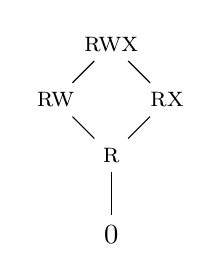
\begin{tikzpicture}[main node/.style={}]
    \node[main node] (rwx) {$\rwx$};
    \node[main node] (rx) [below right of=rwx] {$\rx$};

    \node[main node] (rw) [below left of=rwx,] {$\rw$};
    \node[main node] (r) [below right of=rw] {$\readonly$};
    \node[main node] (0) [below of=r] {$\noperm$};

    \path[every node/.style={font=\sffamily\small}]

    (rw) edge (r)
    (r) edge (0)

    (rwx) edge (rx)

    (rw) edge (rwx)
    (r) edge (rx);
  \end{tikzpicture}

  \caption{Permission hierarchy}
  \label{fig:perm-hier}
\end{wrapfigure}%
%
%%% Seals

Any reasonable capability machine needs a way to set up boundaries between security domains with different authorities.
It also must have a way to cross these boundaries such that (1) the security domain we move from can encapsulate and later regain its authority and (2) the security domain we move to regains all of its authority. 
%The M-Machine~\citep{Dally1997Memo59} inspired capability machine in \citet{skorstengaard_reasoning_2017} uses enter-capabilities to achieve this.
On \trgcm{} we have CHERI-like sealed capabilities to achieve this~\cite{watson_cheri_2015,watson_fast_2016}.
% seals
A sealed capability $\sealed{\sigma,\vsc}$ is a pair of a seal $\sigma$ and a capability $\vsc$.
A sealed capability makes an underlying capability opaque which means that the underlying capability cannot be changed or used for the operations it normally gives permission to.
In other words, the authority the underlying capability represents is encapsulated under the seal.
In order to seal a sealable with a seal $\sigma$, it is necessary to have the authority to do so.
The permission to make sealed capabilities is represented by a sets of seals $\seal{\sigma_\var{base},\sigma_\var{end},\sigma_{\var{current}}}$.
A set of seals is a capability that represents the authority to seal sealables with seals in the range $[\sigma_\var{base},\sigma_\var{end}]$.
In spirit of memory capabilities, a set of seals has a current seal $\sigma_{\var{current}}$ that is selected for use in the next seal operation.
% On \trgcm{}, we represent seals in sets rather than single seals to have a more compact representation of multiple seals and make it possible to have seal allocation (not described here).
As we will see later, sealed capabilities can be unsealed with an \texttt{xjmp}, an operation that operates on a pair of capabilities sealed with the same seal.
The instruction will be explained in more detail below, but essentially, it unseals the pair of capabilities, transfers control to one of them (the code part of the pair) and makes the other one (the data part of the pair) available to the invoked code.
The combination of sealed capabilities and \texttt{xjmp} gives (1) and (2).
\begin{figure}[tb]
  \centering
  \[
  \arraycolsep=1.4pt
  \begin{array}{rrcl l rrcl}
   \addrbnf,\basebnf \in & \Addr & \defeq & \nats & \phantom{mak} & \sealbasebnf, \sigma \in & \Seal & \defeq & \nats\\
    \aendbnf \in & & & \Addr \cup \{\infty \} & & \sealendbnf \in & & & \Seal \cup \{\infty \}\\
    \permbnf \in& \Perm & \defbnf & \rwx \mid \rx \mid \rw \mid \ro \mid \noperm & & &\linbnf & \defbnf & \linear \mid \normal\\
    \vsc \in &\SealableCaps&\defbnf & \multicolumn{6}{l}{((\permbnf,\linbnf),\basebnf,\aendbnf,\addrbnf) \mid \seal{\sealbasebnf,\sealendbnf,\sigma}}\\
    c \in&\Caps& \defbnf &  \SealableCaps \mid \sealed{\sigma,\scbnf} & & w \in &\Word & \defeq & \ints \uplus \Caps\\ 
    r \in& \RegName & \defbnf & \multicolumn{6}{l}{\pcreg \mid \rretd \mid \rretc \mid \rstk \mid \rdata \mid \rtmp{1} \mid \rtmp{2} \mid \dots} \\
    \reg \in &\Reg & \defeq & \RegName \fun \Word & & \mem \in&\Mem & \defeq & \Addr \fun \Word\\
\ms \in  &\MemSeg & \defeq & \Addr \parfun \Word & & \Phi \in & \ExecConf & \defeq & \Mem \times \Reg\\
    &\Conf & \defeq & \multicolumn{6}{l}{\ExecConf \cup \{\failed\} \cup \{\halted\} }
  \end{array}
\]
\[
  \arraycolsep=1.4pt
\begin{array}{rcl}
\multicolumn{3}{l}{    \arraycolsep=0pt
      \com{r} \in  \tRegName \hspace{2.5cm}   \com{\rn} \defbnf \com{r} \mid \nats
}\\
  \Instr &\defbnf & \tjmp{\com{r}} \mid \tjnz{\com{r}}{\com{\rn}} \mid \tmove{\com{r}}{\com{\rn}} \mid \tload{\com{r}}{\com{r}} \mid \tstore{\com{r}}{\com{r}} \mid \tplus{\com{r}}{\com{\rn}}{\com{\rn}} \mid \tminus{\com{r}}{\com{\rn}}{\com{\rn}} \mid\\
         & & \tlt{\com{r}}{\com{\rn}}{\com{\rn}} \mid \tisptr{\com{r}}{\com{r}} \mid\tgetp{\com{r}}{\com{r}} \mid \tgetlin{\com{r}}{\com{r}} \mid \tgetb{\com{r}}{\com{r}} \mid \tgete{\com{r}}{\com{r}} \mid \tgeta{\com{r}}{\com{r}}  \mid \\
  & & \tcca{\com{r}}{\com{n\rn}} \mid \tsetatob{\com{r}} \mid \trestrict{\com{r}}{\com{\rn}} \mid \tcseal{\com{r}}{\com{r}} \mid \txjmp{\com{r}}{\com{r}} \mid  \tsplit{\com{r}}{\com{r}}{\com{r}}{\com{\rn}} \mid\\ 
      & & \tsplice{\com{r}}{\com{r}}{\com{r}} \mid \tfail \mid \thalt 
\end{array}
\]
  \caption{The syntax of our capability machine with seals and linear capabilities.}
  \label{fig:target-syntax}
\end{figure}

%%% Domains
Words on \trgcm{} are capabilities and data (represented by integers $\ints$).
We assume a finite set of register names $\RegName$ containing at least the registers $\pcreg$, $\rretd$, $\rretc$, $\rstk$, $\rdata$, $\rtmp{1}$, and $\rtmp{2}$.
We define register files as functions from register names to words.
Complete memories map all addresses to words and memory segments map some addresses to words (i.e.\ partial functions).
$\trgcm{}$ has two terminated configurations $\halted$ and $\failed$ that respectively signify a successful execution and an execution where something went wrong, e.g.,\ an out-of-bounds memory access.
An executable configuration is a register file and memory pair.

\begin{figure}[p]
  \centering
  \begin{mathpar}
    \inference{\Phi(\pcreg) = ((\perm,\_),\baddr,\eaddr,\aaddr) \\
        \baddr \le \aaddr \le \eaddr \and \perm \in \{\rwx,\rx\}
 }{ \Phi \step \sem{\decInstr{\Phi.\mem(\aaddr)}}(\Phi) }
              \and
              \inference{ \forall \Phi' \neq \failed \ldotp \Phi \nrightarrow \Phi'}
                        {\Phi \step \failed }
  \end{mathpar}
  \[
    \begin{array}{l}
  %   \Phi \step
  % \begin{cases}
  %   \sem{\decInstr{\Phi.\mem(\aaddr)}}(\Phi) &
  %   \arraycolsep=0pt
  %     \begin{array}[t]{l}
  %       \text{if }\Phi(\pcreg) = ((\perm,\_),\baddr,\eaddr,\aaddr) \wedge
  %       \baddr \le \aaddr \le \eaddr \wedge \perm \in \{\rwx,\rx\}
  %     \end{array} \\
  %     \failed & \totherwise
  % \end{cases}\\
  \updPcAddr{\Phi} =
  \begin{cases}
    \Phi\updReg{\pcreg}{w} & \Phi(\pcreg) = ((\perm,\lin),\baddr,\eaddr,\aaddr) \wedge w = ((\perm,\lin),\baddr,\eaddr,\aaddr+1)\\
    \Phi  & \totherwise
  \end{cases}\\
  \linCons{w} =
  \begin{cases}
    0 & \isLinear{w} \\
    w & \totherwise
  \end{cases}\\
  \xjmpres{c_1,c_2,\Phi} =
  \begin{cases}
    \Phi\updReg{\pcreg}{c_1}\updReg{\rdata}{c_2} & \nonExec{c_2} \\
    \failed & \totherwise
  \end{cases}
  \end{array}
\]
  \begin{tabular}{|>{$}c<{$}|>{$}p{3.7cm}<{$}|>{\raggedright\arraybackslash}p{6.7cm}|}
    \hline
    i \in \Instr                                 & \sem{i}(\Phi) & Conditions\\
    \hline
    \halt                                        & \halted & \\
    \hline
    \fail                                        & \failed & \\
    % \hline
    % \move{r}{\rn}                                & \updPcAddr{\Phi\updReg{r}{\rn}} & $\rn \in \ints$\\
    \hline
    \move{r}{\rn}                                & \updPcAddr{}\arraycolsep=0pt\array[t]{rl}(\Phi&\updReg{\rn}{w_2}\\ & \updReg{r}{w_1})\endarray & $\rn \in \RegName$ and $w_1 = \Phi(\rn)$ and $w_2 = \linCons{\Phi(\rn)}$ \\
    \hline
    \load{r_1}{r_2}                              & \updPcAddr{}\arraycolsep=0pt\array[t]{rl}(\Phi&\updReg{r_1}{w_1}\\ &\update{\mem.\aaddr}{w_\aaddr})\endarray & $\Phi(r_2) = ((\perm,\_),\baddr,\eaddr,\aaddr)$ and $\baddr \le \aaddr \le \eaddr$ and $\perm \in \{\rwx,\rw,\rx,\ro\}$ and $w_1 = \Phi.\mem(\aaddr)$ and $\isLinear{w_1} \Rightarrow \perm \in \{\rwx,\rw\}$ and $w_a = \linCons{w_1}$\\
    \hline
    \store{r_1}{r_2}                             & \updPcAddr{}\arraycolsep=0pt\array[t]{rl}(\Phi&\updReg{r_2}{w_2}\\ & \update{\mem.\aaddr}{\Phi(r_2)})\endarray & $\Phi(r_1) = ((\perm,\_),\baddr,\eaddr,\aaddr)$ and $\perm \in \{\rwx,\rw\}$ and $\baddr \le \aaddr \le \eaddr$ and $w_2 = \linCons{\Phi(r_2)}$\\
    \hline
    \geta{r_1}{r_2}                              & \updPcAddr{\Phi\updReg{r_1}{w}} & If $\Phi(r_2) = ((\_,\_),\_,\_,\aaddr)$ or $\Phi(r_2) = \seal{\_,\_,\aaddr}$, then $w = \aaddr$ and otherwise $w = -1$\\
    \hline
    \cca{r}{\rn}                                 &\updPcAddr{\Phi\updReg{r}{w}} & $\Phi(\rn) = n \in \ints$ and either $\Phi(r) = ((\perm,\lin),\baddr,\eaddr,\aaddr)$ or $\Phi(r) = (\sigma_\baddr,\sigma_\eaddr,\sigma)$ and $w = ((\perm,\lin),\baddr,\eaddr,\aaddr + n)$ or $w = (\sigma_\baddr,\sigma_\eaddr,\sigma+n)$, respectively \\
    \hline
    \jmp{r}    &\Phi\arraycolsep=0pt\array[t]{l}\updReg{r}{w}\\\updReg{\pcreg}{\Phi(r)}\endarray & $w = \linCons{\Phi(r)}$\\
    \hline
    \xjmp{r_1}{r_2}                              & \Phi' & $\Phi(r_1) = \sealed{\sigma,c_1}$ and $\Phi(r_2) = \sealed{\sigma,c_2}$ and $w_1 = \linCons{c_1}$ and $w_2 = \linCons{c_2}$ and $\Phi' = \xjmpres{c_1,c_2,\Phi\updReg{r_1,r_2}{w_1,w_2}}$  \\
    \hline
    \tsplit{r_1}{r_2}{r_3}{\rn}                  & \updPcAddr{}\arraycolsep=0pt\array[t]{rl}(\Phi&\updReg{r_3}{w}\\ &\updReg{r_1}{c_1}\\ &\updReg{r_2}{c_2})\endarray & $\Phi(r_3) = ((\perm,\lin),\baddr,\eaddr,\aaddr)$ and $\Phi(\rn) = n \in \nats$ and $\baddr \le n < \eaddr$ and $c_1 = ((\perm,\lin),\baddr,n,\aaddr)$ and $c_2 = ((\perm,\lin),n+1,\eaddr,\aaddr)$ and $w = \linCons{\Phi(r_3)}$\\
    \hline
    \splice{r_1}{r_2}{r_3}                       & \updPcAddr{}\arraycolsep=0pt\array[t]{rl}(\Phi&\updReg{r_2}{w_2}\\ &\updReg{r_3}{w_3}\\ &\updReg{r_1}{c})\endarray& $\Phi(r_2) = ((\perm,\lin),\baddr,n,\_)$ and $\Phi(r_3) = ((\perm,\lin),n+1,\eaddr,\aaddr)$ and $\baddr \le n < \eaddr$ and $c = ((\perm,\lin),\baddr,\eaddr,\aaddr)$ and $w_2,w_3 = \linCons{\Phi(r_2),\Phi(r_3)}$\\
    \hline
    \cseal{r_1}{r_2}                             & \updPcAddr{\Phi\updReg{r_1}{\vsc}} & $\Phi(r_1) \in \SealableCaps$ and $\Phi(r_2) = \seal{\sigma_\baddr,\sigma_\eaddr,\sigma}$ and $\sigma_\baddr \le \sigma \le \sigma_\eaddr$ and $\vsc = \sealed{\sigma,\Phi(r_1)}$ \\
    \hline
    \multicolumn{3}{|c|}{\dots} \\
    \hline
    \_                                           & \failed & \totherwise \\
    \hline
  \end{tabular}
\caption{An excerpt of the operational semantics of \trgcm{}}
  \label{fig:target-op-sem}
\end{figure}
% syntax (instructions)
\trgcm{}'s instruction set is somewhat basic with the instructions one expects on most low-level machines as well as capability-related instructions.
The standard instructions are: unconditional and conditional jump (\texttt{jmp} and \texttt{jnz}), copy between registers (\texttt{move}), instructions that load from memory and store to memory (\texttt{load} and \texttt{store}), and arithmetic operations (\texttt{plus}, \texttt{minus}, and \texttt{lt}).
The simplest of the capability instructions inspect the properties of capabilities: type (\texttt{gettype}), linearity (\texttt{getl}), range (\texttt{getb} and \texttt{gete}), current address or seal (\texttt{geta}) or permission (\texttt{getp}).
The current address (or seal) of a capability (or set of seals) can be shifted by an offset (\texttt{cca}) or set to the base address (\texttt{seta2b}).
The \texttt{restrict} instruction reduces the permission of a capability according to the permission order $\le$.
Generally speaking, a capability machine needs an instruction for reducing the range of authority of a capability.
Because \trgcm{} has linear capabilities, the instruction for this splits the capability in two rather than reducing the range of authority (\texttt{split}).
The reverse is possible using \texttt{splice}.
Sealables can be sealed using \texttt{cseal} and pairs of sealed capabilities can be unsealed by crossing security boundaries (\texttt{xjmp}, see below).
Finally, \trgcm{} has instructions to signal whether an execution was successful or not (\texttt{halt} and \texttt{fail}).

% opsem
The operational semantics of \trgcm{} is displayed in Figure~\ref{fig:target-op-sem}.
The operational semantics is defined in terms of a step relation that executes the next instruction in an executable configuration $\Phi$ which results in a new executable configuration or one of the two terminated configurations.
The executed instruction is determined by the capability in the $\pcreg$ register, i.e.\ $\Phi(\pcreg)$ (we write $\Phi(r)$ to mean $\Phi.\reg(r)$).
In order for the machine to take a step, the capability in the $\pcreg$ must have a permission that allows execution, and the current address of the capability must be within the capability's range of authority.
If both conditions are satisfied, then the word pointed to by the capability is decoded to an instruction which is interpreted relative to $\Phi$.
The interpretations of some of the instructions are displayed in Figure~\ref{fig:target-op-sem}.
In order to step through a program in memory, most of the interpretations use the function $\updPcAddr{}$ which simply updates the capability in the $\pcreg$ to point to the next memory address.
The instructions that stop execution or change the flow of execution do not use $\updPcAddr{}$.
For instance, the \texttt{halt} and \texttt{fail} instructions are simply interpreted as the $\halted$ and $\failed$ configurations, respectively, and they do not use $\updPcAddr{}$.

% move w/ lin
The \texttt{move} instruction simply moves a word from one register to another.
It is, however, complicated slightly by the presence of the non-duplicable linear capabilities.
When a linear capability is moved, the source register must be cleared to prevent duplication of the capability.
This is done uniformly in the semantics using the function $\linCons{}$ that returns $0$ for linear capabilities and is the identity for all other words.
When a word $w$ is transferred on the machine, then the source of $w$ is overwritten with $\linCons{w}$ which clears the source if $w$ was linear and leaves it unchanged otherwise.
In the case of \texttt{move}, the source register $\rn$ is overwritten with $\linCons{\Phi(\rn)}$.

% load w/ lin (and store)
The \texttt{store} and \texttt{load} instructions are fairly standard.
They require a capability with permission to either write or read depending on the operation, they check that the capability points within the range of authority.
Linear capabilities introduce one extra complication for \texttt{load} as it needs to clear the loaded memory address when it contains a linear capability in order to not duplicate the capability.
In this case, we require that the memory capability used for loading also has write-permission.

% geta, cca
The instruction \texttt{geta} projects the current address (or seal) from a capability (or set of seals), and returns $-1$ for data and sealed capabilities.
\texttt{cca} (change current address) changes the current address or seal of a capability or set of seals, respectively, by a given offset.
Note that this instruction does not need to use $\linCons{}$ like the previous ones, because it modifies the capability in-place, i.e.\ the source register is also the target register.
The \texttt{jmp} instruction is a simple jump that just sets register $\pcreg$.

%% Sealing
The operational side of the sealing in \trgcm{} consists of two instructions: \texttt{cseal} for sealing a capability and \texttt{xjmp} for unsealing a pair of capabilities.
% cseal
Given a sealable $\vsc$ and a set of seals where the current seal $\sigma$ is within the range of available seals, the \texttt{cseal} instruction seals $\vsc$ with $\sigma$.
% xjmp
Apart from dealing with linearity, \texttt{xjmp} takes a pair of sealed capabilities, unseals them, and puts one in the $\pcreg$ register and the other in the $\rdata$ register, but only if they are sealed with the same seal and the data capability (the one placed in $\rdata$) is non-executable.
A pair of sealed capabilities can be seen as a closure where the code capability (the capability placed in $\pcreg$) is the program and the data capability is the local environment.
Because of the opacity of sealed capability, the creator of the closure can be sure that execution will start where the code capability points and only in an environment with the related data, i.e.\ sealed with the same seal.
This makes \texttt{xjmp} the mechanism on \trgcm{} that transfers control between security domains.
Opaque sealed capabilities encapsulate a security domain's local state and authority, and they only become accessible again when control is transferred to the security domain.
Some care should be taken for sealing because reusing the same seal for multiple closures makes it possible to jump to the code of one closure with the environment of another.
% xjmp to unseal
\trgcm{} does not have an instruction for unsealing capabilities directly, but it can be (partially) simulated using \texttt{xjmp}.

% split/splice
Instructions for reducing the authority of capabilities are commonplace on capability machines as they allow us to limit what a capability can do before it is passed away.
For normal capabilities, reduction of authority can be done without actually giving up any authority by duplicating the capability first.
With linear capabilities authority cannot be preserved in this fashion as they are non-duplicable.
In order to make a lossless reduction of the range of authority, \trgcm{} provides special hardware support in the form of \texttt{split} and \texttt{splice}.
The \texttt{split} instruction takes a capability with range of authority $[\var{base},\var{end}]$ and an address $n$ and creates two new capabilities, with $[\var{base},n]$ and $[n+1,\var{end}]$ as ranges of authority.
Everything else, i.e.\ permission, linearity and current address, is copied without change to the new capabilities.
With \texttt{split}, we can reduce the range of authority of a linear capability without losing any authority as we retain it in the second capability.
The \texttt{splice} instruction essentially does the inverse of \texttt{split}.
Given two capabilities with adjacent ranges of authority and the same permissions and linearity, \texttt{splice} splices them together into one capability.
The two instructions work in the same way for seal sets.
We do not provide special support for lossless reduction of capability permissions, but this could probably be achieved with more fine-grained permissions.
This would also allow linear capabilities to have aliases, but only by linear capabilities with disjoint permissions.

\begin{jversion}
% The remaining instructions
  The interpretation of the remainder of the instructions are displayed in Appendix~\ref{app:instr-interpretation}.
  The instructions $\tgetb{}{}$, $\tgete{}{}$, $\tgetlin{}{}$, and $\tgetp{}{}$ all project information about capabilities.
  The $\tgetb{}{}$ and $\tgete{}{}$ instructions, respectively, project the base and end address of the range of authority.
  The linearity of a permission is projected with $\tgetlin{}{}$, and finally the permission is projected with $\tgetp{}{}$.
  The instructions $\tgetb{}{}$ and $\tgete{}{}$ also work on sets of seals.
  The instruction $\tisptr{}{}$ returns an integer representation of the type of a word which allows programs to be defensive in the sense that they can check whether a word is a capability before they use it.
  \trgcm{} also has arithmetic instructions $\tplus{}{}{}$, $\tminus{}{}{}$, and $\tlt{}{}{}$.
  The latter instruction compares two numbers and writes 1 or 0 to a target register depending on whether one number is less than the other.
  The instruction $\tsetatob{}$ sets the current address (or seal) of a capability (or set of seals) to the base address of the range of authority (or range of seals).
  This instruction makes it easy to work relatively to the base address of a capability.
  This instruction is not strictly necessary as it can be emulated with other instructions.
  Finally, we have the $\trestrict{}{}$ instruction which restricts the permission of a capability according to the $\le$ relation.
\end{jversion}

\begin{jversion}
  \subsection{The purpose of sealing}
  \label{sec:purpose-sealing}
  % Sealing example:
  To motivate the necessity of an encapsulation mechanism like sealing, consider the following example.
  We, a trusted piece of code, want to transfer control to code that we distrust, and we want to give them the means to return to us.
  That is, we need to give them a return capability.
  If we did not have an encapsulation mechanism, our only option would be to give them an executable capability for the address we want them to return to.
  The untrusted code could use the return capability as intended, but it could also manipulate and make it point to a different address of our code.
  Jumping to such a capability would cause an the program to execute in a way we did not intend for it.
  Further in order to be able to retrieve our capabilities from before transferring control, we would have to store the capabilities somewhere accessible from the return capability.
  However, the untrusted code would have access to all this through the return capability because it gives the same authority to us as the untrusted code.
  This is why, any reasonable capability machine must have an encapsulation mechanism to allow programs to make boundaries between security domains.
  
  In the example, we could seal the return capability to establish a boundary.
  Specifically, it would prevent the untrusted code from changing the target of the return capability forcing them to return to the point we specified.
  It would also prevent the untrusted code from reading our capabilities.
  All in all, this means that we can transfer control to untrusted code without giving up our capabilities or handing them over.

  \trgcm{} does not have a direct unsealing instruction, but it is still possible to emulate a limited unsealing mechanism.
  Say you have a sealed non-executable word $\sealed{\sigma,w}$ as well as a set of seals $\seal{\sigma_\baddr,\sigma_\eaddr, \sigma}$ that contains $\sigma$, i.e.\ $\sigma \in [\sigma_\baddr,\sigma_\eaddr]$.
  Now assume part of the code would like to have access to $w$ in $\rdata$.
  Take a capability for this code, possibly by adjusting the pc, and seal it with $\sigma$.
  Now you have the data part and the code part of a sealed capability pair, so you can $\txjmp{}{}$ to it which unseals the data capability and puts it in $\rdata$ for your code to use.
  Sealed executable capabilities cannot be unsealed in the same way because $\txjmp{}{}$ fails if the data capability is executable.
  However, given a sealed executable capability $\sealed{\sigma,c}$ and a set of seals that contains $\sigma$, we can still construct the data part of the sealed capability pair.
  This means that we can execute the code the capability points to together with data that it was not intended to be used with.

  Sealing is meant for encapsulation, but it relies on seals being kept private as illustrated by the unsealing emulation.
  For this reason, it is important that the system is initialised such that each component has access to unique seals.
  We return to this in \sectionname~\ref{sec:well-form-reas}.
\end{jversion}

\begin{jversion}
\subsection{Decoding and encoding functions}
The operational semantics of the capability machine uses the function $\decInstr{}$ to decode instructions.
We also assume a function $\encInstr{}$ to make it easy to specify programs in terms of instructions.
Rather than specifying a decode function and an encode function, we assume that they are given with certain properties.
The $\decInstr{} : \Word \fun \Instr$ should be surjective and injective for all non-$\fail$ instructions.
Further, it should decode all capabilities as the $\fail$ instruction, i.e.\
\[
\forall c \in \Caps \ldotp \decInstr{c} = \fail
\]
The $\encInstr{} : \Instr \fun \ints$ function should be injective, and it should be defined so $\decInstr{}$ is its left inverse, i.e.
\[
\forall i \in \Instr \ldotp \decInstr{}(\encInstr{i}) = i
\]

These assumptions are sufficient to construct program examples and run them on the machine.
The $\encInstr{}$ function allows us to specify the program ``abstractly'' in terms of instructions rather than machine words.
As the $\decInstr{}$ function is the left inverse of $\encInstr{}$, we can even execute the program in the operational semantics without ever worrying about what the actual encoding is.
%This is not to say that encoding is an easy problem. There are many things to get.

The machine also assumes decode and encode functions for permissions $\decPerm{} : \Perm \fun \ints$ and $\encPerm{} : \ints \fun \Perm$.
We assume the $\decPerm{}$ function to be the left inverse of $\encPerm{}$ and surjective. For $\encPerm{}$, we assume it is surjective and that it does not encode anything to the $\tgetp{}{}$ error value -1, i.e.
\[
  \forall \perm \in \Perm \ldotp \encPerm{\perm} \neq -1
\]
For linearity we assume similar functions.

Finally in the interpretation of $\tisptr{}{}$, the machine uses an encode function for word types $\encType{}$.
This function encodes each kind of word as an integer.
This is very much like the previous functions.
It encodes each kind of word differently and all words of the same kind to the same integer.
\end{jversion}

\subsection{Components, linking, programs, and contexts }
\label{subsec:components-linking}
The executable configuration describes the machine state, but it does not make it clear what components run on the machine and how they interact with each other.
To clarify this, we introduce notions of components and programs from which we construct executable configurations.
A component (defined in Figure~\ref{fig:target-component-and-linking}) is basically a program with entry points in the form of imports that need to be linked.
It has exports that can satisfy the imports of other components.
% Structure
A base component $\comp_0$ consists of a code memory segment, a data memory segment, a list of imported symbols, a list of exported symbols, two lists specifying the available seals\footnote{We will return to the seals in Section~\ref{sec:form-secur-with}.}, and a set of all the linear addresses (addresses governed by a linear capability).
The import list specifies where in memory imports should be placed, and imports are matched to exports via their symbols.
The exports are words each associated with a symbol.
%base = library
A component is either a library component (without a main entry point) or an incomplete program with a main in the form of a pair of sealed capabilities.
The latter can be seen as a program that still needs to be linked with libraries.
% Linking .
Components are combined into new components by linking them together, as long as only one is an incomplete program with a main.
Two components can be linked when their memories, seals, and linear addresses are disjoint.
They are combined by taking the union of each of their constituents.
For every import that is satisfied by an export of the other component, the data memory is updated to have the exported word on the imported address.
The satisfied imports are removed from the import list in the resulting linked component and the exports are updated to be the exports of the two components.

% Programs
We can now define the notion of a program as well as a context.
\begin{definition}[Programs and Contexts]
  \label{def:program-and-context}
  A \emph{program} is a component $(\comp_0,c_{\mathrm{main},c}, c_{\mathrm{main},d})$ with an empty import list.
  A \emph{context} for a component $\comp$ is a component $\comp'$ such that $\comp \bowtie \comp'$ is a program.
\end{definition}
% Getting an executable from a component - postpone this to later, but mention:
% write xor exec
How a program is initialised to create an executable configuration, is discussed in Section~\ref{sec:form-secur-with}.
% We will, however, at this point mention that all programs will be instrumented as Write-XOR-Execute,{Do we have a reference for this?} i.e.\ there will only be read-execute capabilities for the code and read-write capabilities for the data.
%Further, we will only consider a specific class of well-formed components, but we will get back to this.
Some simplifications have been made in this presentation of \trgcm{}. See \citet{technical_report_popl} for details.
\begin{figure}[tb]
  \centering
  \[
    \begin{array}{rl c rl c rl}
    s &\in \Symbol & \phantom{make} &
    \mathrm{import} &\mathrel{::=} a \mapsfrom s & \phantom{make} &
    \mathrm{export} &\mathrel{::=} s \mapsto w\\
    \comp_0 & \multicolumn{7}{l}{\mathrel{::=} (\mscode,\msdata,\overline{\mathrm{import}},\overline{\mathrm{export}},\sigrets,\sigcloss,A_\linear)}\\
    \comp & \multicolumn{7}{l}{\mathrel{::=} \comp_0 \mid  (\comp_0,c_{\mathrm{main},c}, c_{\mathrm{main},d})}
  \end{array}
\]
\vspace{0.5cm}
\begin{mathpar}
  \inference{
    \comp_0 = (\mscode[1], \msdata[1], \overline{\var{import}_1}, \overline{\var{export}_1}, \sigrets[1], \sigcloss[1],A_{\linear,1})\\
    \comp_0' = (\mscode[2], \msdata[2], \overline{\var{import}_2}, \overline{\var{export}_2}, \sigrets[2], \sigcloss[2],A_{\linear,2})\\
    \comp_0'' = (\mscode[3], \msdata[3], \overline{\var{import}_3}, \overline{\var{export}_3}, \sigrets[3], \sigcloss[3],A_{\linear,3})\\
    \mscode[3] = \mscode[1] \uplus \mscode[2] \\
    \msdata[3] = (\msdata[1] \uplus \msdata[2])[a \mapsto w \mid (a \mapsfrom s) \in (\overline{\var{import}_1} \cup \overline{\var{import}_2}), (s \mapsto w) \in \overline{\var{export}}_3] \\
    \overline{\var{export}_3} = \overline{\var{export}_1} \cup \overline{\var{export}_2}&
    \overline{\var{import}_3} = \{ a \mapsfrom s \in (\overline{\var{import}_1} \cup \overline{\var{import}_2}) \mid s \mapsto \_ \not\in \overline{\var{export}_3} \}\\
    \sigrets[3] = \sigrets[1] \uplus \sigrets[2] &
    \sigcloss[3] = \sigcloss[1] \uplus \sigcloss[2] &
    A_{\linear,3} = A_{\linear,1} \uplus A_{\linear,2}\\
    \dom(\mscode[3]) \mathrel{\#} \dom(\msdata[3]) & \sigrets[3] \mathrel{\#} \sigcloss[3]
  } {
    \comp_0'' = \comp_0 \bowtie \comp_0'
  }
  \and
  \inference{
    \comp_0'' = \comp_0 \bowtie \comp_0'
  }{
    (\comp_0'',c_{\mathrm{main},c}, c_{\mathrm{main},d}) = \comp_0 \bowtie (\comp_0',c_{\mathrm{main},c}, c_{\mathrm{main},d}) = (\comp_0,c_{\mathrm{main},c}, c_{\mathrm{main},d}) \bowtie \comp_0'
  }
  \end{mathpar}
% \begin{definition}[Plugging a program into a context]
%   When $\var{comp'}$ is a context for component $\comp$ and $\comp' \bowtie \comp \rightsquigarrow \Phi$, 
%   then we write $\plug{\comp'}{\comp}$ for the execution configuration $\Phi$.
% \end{definition}
  \caption{Components and linking of components.}
  \label{fig:target-component-and-linking}
\end{figure}

%\FloatBarrier
% \begin{itemize}
% \item present our \emph{target language} and its operational semantics (excerpts)
% \item mention roughly what components look like
% \end{itemize}
\section{Linear Stack and Return Capabilities}
\label{sec:stktokens-explained}
In this section, we introduce our calling convention \stktokens{} that ensures LSE and WBCF.
We will gradually explain each of the security measures \stktokens{} takes and motivate them with the attacks they prevent.

\begin{figure}
  \centering
  \begin{subfigure}{0.4\linewidth}
    \centering
    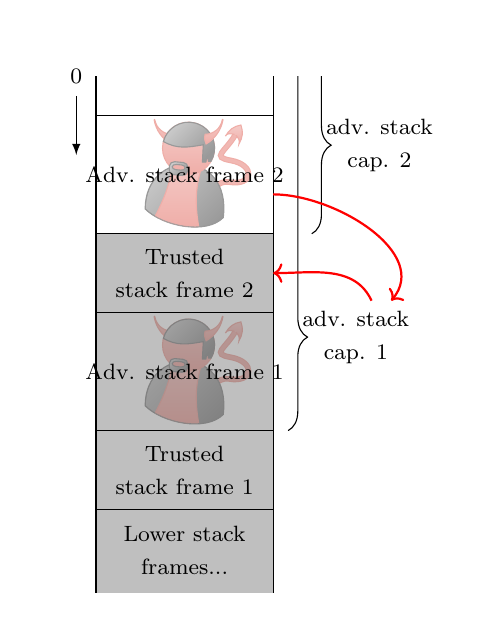
\begin{tikzpicture}[scale=.5, every node={scale=.5}]
      % recurrent parts
      \draw (-0.5,13) node {\footnotesize 0};
      \draw (-0.5,12.5) edge[thin,-latex] (-0.5,11);
      \stdstackstart[13]
      \inactsf{(0,2)}{(4.5,4)} {\footnotesize Trusted\\ \footnotesize stack frame 1}
      \inactadv{(0,4)}{(4.5,7)} {\footnotesize Adv. stack frame 1}
      \inactsf{(0,7)}{(4.5,9)} {\footnotesize Trusted \\ \footnotesize stack frame 2}
      \actadv{(0,9)}{(4.5,12)} {\footnotesize Adv. stack frame 2}

      % Stack pointer 1
      \begin{scope}
        \clip (4.6,4) rectangle (9,13);
        \capbracebot{(4.6,4)}{(4.6,13.5)}{adv. stack\\\footnotesize cap. 1}
      \end{scope}
      Stack pointer 2
      \begin{scope}
        \clip (4.8,4) rectangle (9,13);
        \capbrace{(5.2,9)}{(5.2,13.5)}{adv. stack\\\footnotesize cap. 2}
      \end{scope}

      \draw[red,thick,->] (4.5,10) to[out=0,in=50] node[midway,right] {} (7.5,7.3);
      \draw[red,thick,->] (7,7.3) to[out=115,in=0] node[midway,right] {} (4.5,8);
    \end{tikzpicture}
    \caption{An adversary uses a previous stack frame's stack pointer.}
    \label{fig:stack-ptr-abuse}
  \end{subfigure}
  \begin{subfigure}{0.18\linewidth}
    \phantom{testtestes}
  \end{subfigure}
  \begin{subfigure}{0.4\linewidth}
    \centering
    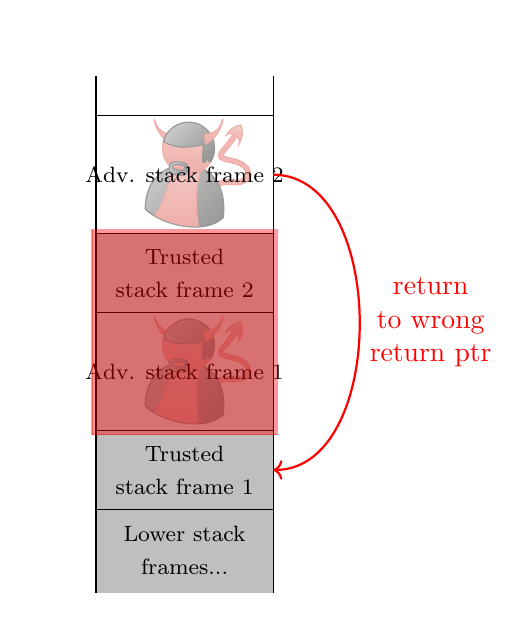
\begin{tikzpicture}[scale=.5, every node={scale=.5}]
      % recurrent parts
      \stdstackstart[13]
      \inactsf{(0,2)}{(4.5,4)} {\footnotesize Trusted\\ \footnotesize stack frame 1}
      \inactadv{(0,4)}{(4.5,7)} {\footnotesize Adv. stack frame 1}
      \inactsf{(0,7)}{(4.5,9)} {\footnotesize Trusted \\ \footnotesize stack frame 2}
      \actadv{(0,9)}{(4.5,12)} {\footnotesize Adv. stack frame 2}
      \fill[red,draw=red,opacity=.4] (-.1,3.9) rectangle (4.6,9.1);
      \draw[red,thick,->] (4.5,10.5) to[out=0,in=0] node[midway,right,align=center] {return\\ to wrong\\ return ptr} (4.5,3);
    \end{tikzpicture}
    \caption{An adversary jumps to a previous stack frame's stack pointer.}
    \label{fig:ret-ptr-abuse}
  \end{subfigure}
  
  \caption{Possible ways to abuse stack and return capabilities.}
  \label{fig:stack-ret-ptr-abuse}
\end{figure}

\stktokens{} is based on a traditional single stack, shared between all components.
To explain the technique, let us first consider how we might already add extra protection to stack and return pointers on a capability machine.
First, we replace stack pointers with stack capabilities.
When a new stack frame is created, the caller provisions it with a stack capability, restricted to the appropriate range, i.e.\ it does not cover the caller's stack frame.
Return pointers, on the other hand, are replaced by a pair of sealed return capabilities, as we already explained in Section~\ref{sec:purpose-sealing}.
% KJAA: Again with the sealed pair. Again, this idea is unclear.
They form an opaque closure that the callee can only jump to, and the caller's data becomes available to the caller's return code. 

%informally explain how an adversary may try to abuse stack and return caps
While the above adds extra protection, it is not sufficient to enforce WBCF and LSE.
Untrusted callees receive a stack capability and a return pair that they are supposed to use for the call.
However, a malicious callee (which we will refer to as an adversary\footnote{See Section~\ref{sec:well-form-reas} for more details on our attacker model.}) can store the provided capabilities on the heap in order to use them later.
Figure~\ref{fig:stack-ret-ptr-abuse} illustrates two examples of this.
In both examples our component and an adversarial component have been taking turns calling each other, so the stack now contains four stack frames alternating between ours and theirs.
The figure on the left (Figure~\ref{fig:stack-ptr-abuse}) illustrates how we try to ensure LSE by restricting the stack capability to the unused part before every call to the adversary.
However, restricting the stack capability does not help when we, in the first call, give access to the part of the stack where our second stack frame will reside as nothing prevents the adversary from duplicating and storing the stack pointer.
Generally speaking, we have no reason to ever trust a stack capability received from an untrusted component as that stack capability may have been duplicated and stored for later use.
In the figure on the right (Figure~\ref{fig:ret-ptr-abuse}), we have given the adversary two pairs of sealed return capabilities, one in each of the two calls to the adversarial component.
The adversary stores the pair of sealed return capabilities from the first call in order to use it in the second call where they are not allowed.
The figure illustrates how the adversarial code uses the return pair from the first call to return from the second call and thus break WBCF.

% Informally explain how we prevent this using linear capabilities
As the examples illustrate, this naive use of standard memory and object capabilities does not provide sufficient guarantees to enforce LSE and WBCF.
The problem is essentially that the stack and return pointers that a callee receives from a caller remain in effect after their intended lifetime: either when the callee has already returned or when they have themselves invoked other code. 
Linear capabilities offer a form of revocation\footnote{Revocation in the sense that if we hand out a linear capability and later get it back, then the receiver no longer has it or a copy of it as it is non-duplicable.} that can be used to prevent this from happening.

% Stack capability linear
The linear capabilities are put to use by requiring the stack capability to be linear.
On call, the caller splits the stack capability in two: one capability for their local stack frame and another one for the unused part of the stack.
The local stack frame capability is sealed and used as the data part of the sealed return pair.
The capability for the remainder of the stack is given to the callee.
% Prevention of left attack non-aliasing of linear capabilities - token like (ensuring LSE)
Because the stack capability is linear, the caller knows that the capability for their local stack frame cannot have an alias.
This means that an adversary would need the stack capability produced by the caller in order to access their local data.
The caller gives this capability to the adversary only in a sealed form, rendering it opaque and unusable.
This is illustrated in Figure~\ref{fig:stack-ptr-abuse-prev} and prevents the issue illustrated in Figure~\ref{fig:stack-ptr-abuse}.

% Prevention of attack 2
In a traditional calling convention with a single stack, the stack serves as a call stack keeping track of the order calls were made in and thus in which order they should be returned to.
A caller pushes a stack frame to the stack on call and a callee pops a stack frame from the stack upon return.
However without any enforcement, there is nothing to prevent a callee from returning from an arbitrary call on the call stack.
This is exactly what the adversary does in Figure~\ref{fig:ret-ptr-abuse} when they skip two stack frames.
In the presence of adversarial code, we need some mechanism to enforce that the order of the call stack is kept.
One way to enforce this would be to hand out a token on call that can only be used when the caller's stack frame is on top of the call stack.
The callee would have to provide this token on return to prove that it is allowed to return to the caller, and on return the token would be taken back by the caller to prevent it from being spent multiple times.
As it turns out, the stack capability for the unused part of the stack can be used as such a token in the following way:
On return the callee has to give back the stack capability they were given on invocation.
When the caller receives a stack capability back on return, they need to check that this token is actually spendable, i.e.\ check whether their stack frame is on top of the call stack or not.
They do this by attempting to restore the stack capability from before the call by splicing the return token with the stack capability for the local stack frame which at this point has been unsealed again.
If the splice is successful, then the caller knows that the two capabilities are adjacent. On the other hand, if the splice fails, then they are alerted to the fact that their stack frame may not be the topmost.
\stktokens{} uses this approach; and as illustrated in Figure~\ref{fig:ret-ptr-abuse-prev}, it prevents the issue in Figure~\ref{fig:ret-ptr-abuse} as the adversary does not return a spendable token when they return.
\begin{figure}
  \centering
  \begin{subfigure}{0.4\linewidth}
    \centering
    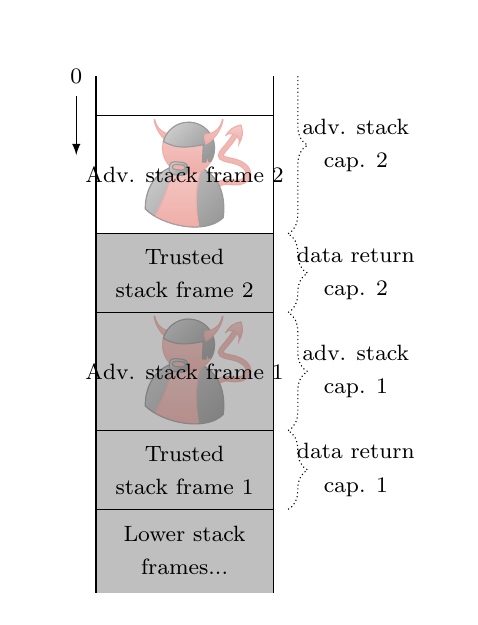
\begin{tikzpicture}[scale=.5, every node={scale=.5}]
      % recurrent parts
      \draw (-0.5,13) node {\footnotesize 0};
      \draw (-0.5,12.5) edge[thin,-latex] (-0.5,11);
      \stdstackstart[13]
      \inactsf{(0,2)}{(4.5,4)} {\footnotesize Trusted\\ \footnotesize stack frame 1}
      \inactadv{(0,4)}{(4.5,7)} {\footnotesize Adv. stack frame 1}
      \inactsf{(0,7)}{(4.5,9)} {\footnotesize Trusted \\ \footnotesize stack frame 2}
      \actadv{(0,9)}{(4.5,12)} {\footnotesize Adv. stack frame 2}

      \sealsymb{(4.9,3)}
      \lincapbrace{(4.6,2)}{(4.6,4)}{data return\\\footnotesize cap. 1}

      % Stack pointer 1
      \sealsymb{(4.9,5.5)}
      \lincapbrace{(4.6,4)}{(4.6,7)}{adv. stack\\\footnotesize cap. 1}
      % return cap
      \sealsymb{(4.9,8)}
      \lincapbrace{(4.6,7)}{(4.6,9)}{data return\\\footnotesize cap. 2}
     %  Stack pointer 2
      \begin{scope}
        \clip (4.8,4) rectangle (9,13);
        \lincapbrace{(4.6,9)}{(4.6,13.5)}{adv. stack\\\footnotesize cap. 2}
      \end{scope}

    \end{tikzpicture}
    \caption{The non-duplicable linear stack capability for the trusted code's
      stack frame and the opacity of sealed capabilities ensures LSE.}
    \label{fig:stack-ptr-abuse-prev}
  \end{subfigure}
  \begin{subfigure}{0.18\linewidth}
    \phantom{testtestes}
  \end{subfigure}
  \begin{subfigure}{0.4\linewidth}
    \centering
    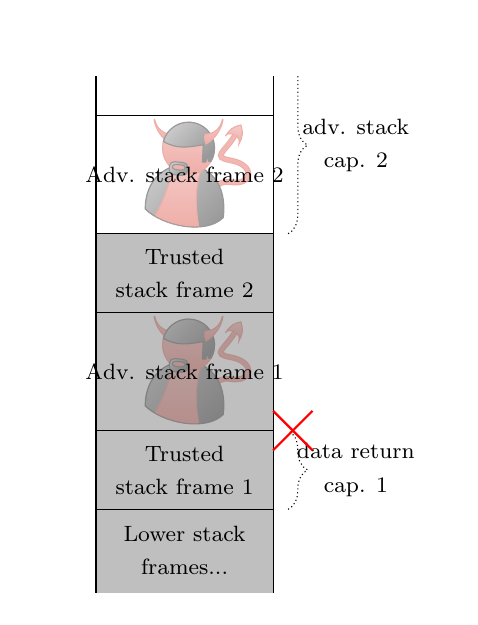
\begin{tikzpicture}[scale=.5, every node={scale=.5}]
      % recurrent parts
      \stdstackstart[13]
      \inactsf{(0,2)}{(4.5,4)} {\footnotesize Trusted\\ \footnotesize stack frame 1}
      \inactadv{(0,4)}{(4.5,7)} {\footnotesize Adv. stack frame 1}
      \inactsf{(0,7)}{(4.5,9)} {\footnotesize Trusted \\ \footnotesize stack frame 2}
      \actadv{(0,9)}{(4.5,12)} {\footnotesize Adv. stack frame 2}

      \lincapbrace{(4.6,2)}{(4.6,4)}{data return\\\footnotesize cap. 1}

     %  Stack pointer 2
      \begin{scope}
        \clip (4.8,4) rectangle (9,13);
        \lincapbrace{(4.6,9)}{(4.6,13.5)}{adv. stack\\\footnotesize cap. 2}
      \end{scope}

      \redcross{(5,4)}
    \end{tikzpicture}
    \caption{The trusted caller fails to splice the stack capability returned by
    the adversary with the capability for the trusted caller's local stack frame.}
    \label{fig:ret-ptr-abuse-prev}
  \end{subfigure}
  \caption{Abuse of stack and return capabilities prevention.}
\end{figure}

% Non-empty trusted stack frames.
In order for a call to have a presence on the call stack, its stack frame must be non-empty.
We cannot allow empty stack frames on the call stack, because then it would be impossible to tell whether the topmost non-empty stack frame has an empty stack frame on top of it.
Non-empty stack frames come naturally in traditional C-like calling convention as they keep track of old stack pointers and old program counters on the stack, but in \stktokens{} these things are part of the return pair which means that a caller with no local data may only need an empty stack frame.
This means that a caller using \stktokens{} needs to take care that their stack frame is non-empty in order to reserve their spot in the return order.
There is also a more practical reason for a \stktokens{} caller to make sure their stack frame is non-empty: They need a bit of the stack capability in order to perform the splice that verifies the validity of the return token.

% known stack base
% + more
At this point, the caller checks that the return token is adjacent to the stack capability for the caller's local stack frame and they have the means to do so.
However, this still does not ensure that the caller's stack frame is on top of the call stack.
The issue is that stack frames may not be tightly packed leaving space between stack frames in memory.
An adversarial callee may even intentionally leave a bit of space in memory above the caller's stack frame, so that they can later return out of order by returning the bit of the return token for the bit of memory left above the caller's stack frame.
This is illustrated in Figure~\ref{fig:stk-base-abuse}: In Figure~\ref{fig:stack-base-abuse-a}, a trusted caller has called an adversarial callee.
The adversary calls the trusted code back, but first they split the return token in two and store on the heap the part for the memory adjacent to the trusted caller's call frame (Figure~\ref{fig:stack-base-abuse-b}).
The trusted caller calls the adversary back using the precautions we have described so far (Figure~\ref{fig:stack-base-abuse-c}).
At this point (Figure~\ref{fig:stack-base-abuse-b}), the adversary has access to a partial return token adjacent to the trusted caller's first stack frame which allows the adversary to return from this call breaking WBCF.

For the caller to be sure that there are no hidden stack frames above its own, they need to make sure that the return token is exactly the same as the one they passed to the callee.
In \stktokens{}, the base address of the stack capability is fixed as a compile-time constant (Note: the stack grows downwards, so the base address of the stack capability is the top-most address of the stack). 
The caller verifies the validity of the return token by checking whether the base address of a returned token corresponds to this fixed base address, which was the base address for the return token they gave to the callee.
In the scenario we just sketched, the caller would be alerted to the attempt to break WBCF when the base address check of the return token fails in Figure~\ref{fig:stack-base-abuse-d}.

% Where do we get the stack pointer from, how can we know it is linear
% The other attack.
% At this point, the caller is able to verify whether a return token is spendable which allows them to decide whether they have the topmost stack frame on a call stack.
% However, in order to have WBCF there should only be one call stack, so the caller should also be able to verify that they have the top stack frame on the call stack used by all well-behaved components.
% In case a trusted component did not start the execution on the machine, i.e.\ they were called by another component, then the trusted component has no way to be sure whether the stack capability passed to them corresponds to the one and only call stack.
% To illustrate how an adversarial component can break WBCF by using multiple different stack capabilities consider this example: An adversary calls a trusted component with a callback and some linear capability that they claim is the stack capability.
% The trusted component executes using the stack capability given to them and at some point they invoke the callback, creating return tokens and so on.
% The adversary stores the return pair and return token and calls another trusted component but with a new callback and a new linear capability that they claim is the stack capability.
% Again, this trusted component also executes using the stack capability given to them and at some point they too invoke the callback, taking all the precautions we have described so far.
% At this point, the adversary has everything they need to return from either of the two callbacks.
% Specifically, they could return from the first callback invocation before they have returned from the second, breaking WBCF.
% From a high-level perspective, the problem is that both trusted components will be able to verify that they have the top stack frame on the call stack.
% They are both correct as the adversarial component has created two call stacks, one for each of the components.
% In order to solve this problem, the well-behaved code needs to somehow agree on the call stack.
% We do this by statically deciding on a global base address for the stack which is used for the entirety of the execution.
% A caller makes sure that they are using the correct stack by checking that the base address of the stack capability they receive corresponds to the global stack base address.
% This also means that on every return, the caller will check whether the return token's base address is equal to the global stack address.

In \stktokens{}, the stack memory is only referenced by a single linear stack capability at the start of execution.
Because of this, the return token can be verified simply by checking its base address and splicing it with the caller's stack frame.
There is no need to check linearity because only linear capabilities to this memory exist.

% Return pointers/return seals
The return pointer in the \stktokens{} scheme is a pair of sealed capabilities where the code part of the pair is the old program counter, and the data part is the stack capability for the local stack frame of the caller.
Both of the capabilities in the pair are sealed with the same seal.
% One seal per return point
All call points need to be associated with a unique seal (a return seal) that is only used for the return capabilities for that particular call point.
The return seal is what associates the stack frame on the call stack with a specific call point in a program, so if we allowed return seals to be reused, it would be possible to return to a different call point than the one that gave rise to the stack frame, breaking WBCF.
For similar reasons, we cannot allow return seals to be used to seal closures.
% Don't be stupid
Return seals should never be leaked to adversarial code as this would allow them to unseal the local stack frame of a caller breaking LSE.
This goes for direct leaks (leaving a seal in a register or writing it to adversarial memory), as well as indirect leaks (leaking a capability for reading, either directly or indirectly, a return seal from memory).

% Note about them vs us, we do nothing that they couldn't do
We have sometimes phrased the description of the \stktokens{} calling scheme in terms of ``them vs us''.
This may have created the impression of an asymmetric calling convention that places a special status on trusted components allowing them to protect themselves against adversaries.
However, \stktokens{} is a modular calling scheme: no restriction is put on adversarial components that we do not expect trusted components to meet.
Specifically, we are going to assume that both trusted and adversarial components are initially syntactically well-formed (described in more detail in Section~\ref{sec:well-form-reas}) which basically just restrict adversarial components to not break machine guarantees initially (e.g.\ no aliases for linear capabilities or access to seals of other components).
This means that any component can ensure WBCF and LSE by employing \stktokens{}.

% KJAA: ^-- Assuming that there is a global stack address capability, no?
% Can I "suddenly" begin to impose \stktokens{}?

% Summary of CC
To summarise, \stktokens{} consists of the following measures:
\begin{enumerate}
\item \label{item:check-stkb} Check the base address of the stack capability before and after calls.
\item \label{item:non-empty-sf} Make sure that local stack frames are non-empty.
\item \label{item:return-data} Create token and data return capability on call: split the stack capability in two to get a stack capability for your local stack frame and a stack capability for the unused part of the stack. The former is sealed and used for the data part of the return pair.
\item \label{item:return-code} Create code return capability on call: Seal the old program counter capability.
\item Reasonable use of seals: Return seals are only used to seal old program counter capabilities, every return seal is only used for one call site, and they are not leaked.
\end{enumerate}
Item~\ref{item:check-stkb}-\ref{item:return-code} are captured by the code in Figure~\ref{fig:call-code} , except for checking stack base before calls.
We do not include this check because it only needs to happen once between two calls, so that the check after a call suffices if the stack base is not changed subsequently.

\begin{figure}
  \centering
  \begin{subfigure}{0.23\linewidth}
    \centering
    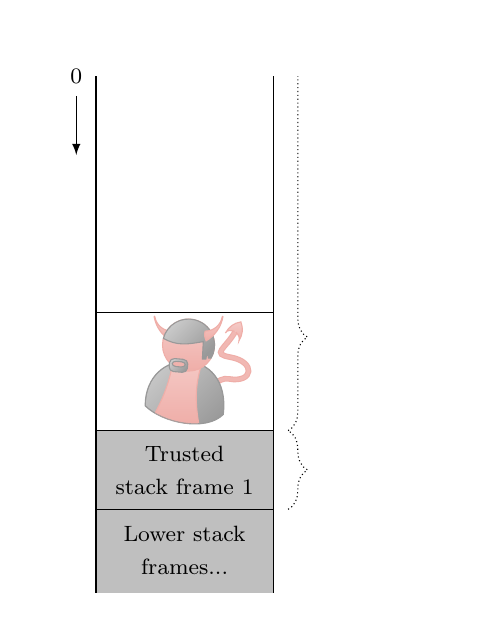
\begin{tikzpicture}[scale=.5, every node={scale=.5}]
      % recurrent parts
      \draw (-0.5,13) node {\footnotesize 0};
      \draw (-0.5,12.5) edge[thin,-latex] (-0.5,11);
      \stdstackstart[13]
      \inactsf{(0,2)}{(4.5,4)} {\footnotesize Trusted\\ \footnotesize stack frame 1}
      \actadv{(0,4)}{(4.5,7)}{}

      \sealsymb{(4.9,3)}
      \lincapbrace{(4.6,2)}{(4.6,4)}{}
      \begin{scope}
        \clip (4.8,1) rectangle (9,13);
      \lincapbracebot{(4.6,4)}{(4.6,13.5)}{}
      \end{scope}

    \end{tikzpicture}
    \caption{}
    \label{fig:stack-base-abuse-a}
  \end{subfigure}
  \begin{subfigure}{0.24\linewidth}
    \centering
    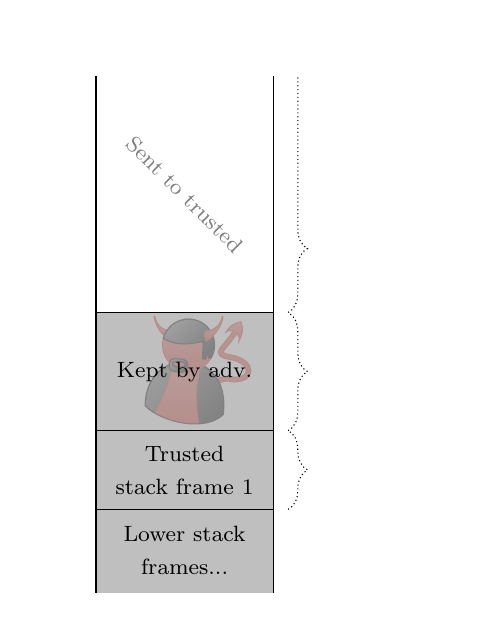
\begin{tikzpicture}[scale=.5, every node={scale=.5}]
      % recurrent parts
      \stdstackstart[13]
      \inactsf{(0,2)}{(4.5,4)} {\footnotesize Trusted\\ \footnotesize stack frame 1}
      \inactadv{(0,4)}{(4.5,7)}{\footnotesize Kept by adv.}
      \node[opacity=0.5,rotate=-45] at (2.25,10) {\footnotesize Sent to trusted};

      \sealsymb{(4.9,3)}
      \lincapbrace{(4.6,2)}{(4.6,4)}{}
      \lincapbrace{(4.6,4)}{(4.6,7)}{}
      
      \begin{scope}
        \clip (4.8,1) rectangle (9,13);
      \lincapbracebot{(4.6,7)}{(4.6,13.5)}{}
      \end{scope}

    \end{tikzpicture}
    \caption{}
    \label{fig:stack-base-abuse-b}
  \end{subfigure}
  \begin{subfigure}{0.24\linewidth}
    \centering
    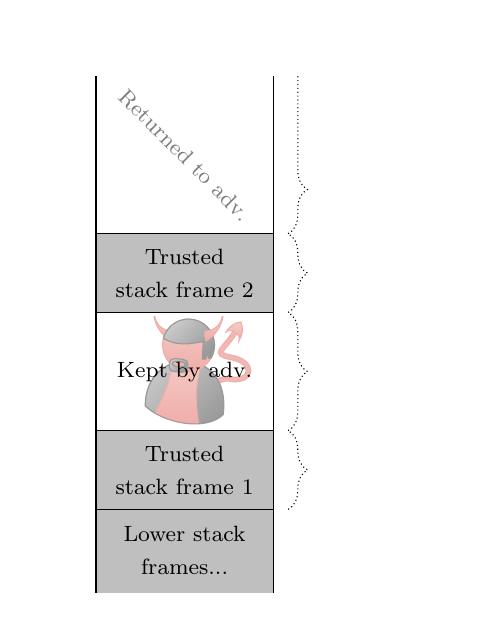
\begin{tikzpicture}[scale=.5, every node={scale=.5}]
      % recurrent parts
      \stdstackstart[13]
      \inactsf{(0,2)}{(4.5,4)} {\footnotesize Trusted\\ \footnotesize stack frame 1}
      \actadv{(0,4)}{(4.5,7)}{\footnotesize Kept by adv.}
      \inactsf{(0,7)}{(4.5,9)} {\footnotesize Trusted\\ \footnotesize stack frame 2}
      \node[opacity=0.5,rotate=-45] at (2.25,11) {\footnotesize Returned to adv.};
      \sealsymb{(4.9,3)}
      \lincapbrace{(4.6,2)}{(4.6,4)}{}
      \lincapbrace{(4.6,4)}{(4.6,7)}{}

      \sealsymb{(4.9,8)}
      \lincapbrace{(4.6,7)}{(4.6,9)}{}
      \begin{scope}
        \clip (4.8,1) rectangle (9,13);
        \lincapbracebot{(4.6,9)}{(4.6,13.5)}{}
      \end{scope}

    \end{tikzpicture}
    \caption{}
    \label{fig:stack-base-abuse-c}
  \end{subfigure}
  \begin{subfigure}{0.24\linewidth}
    \centering
    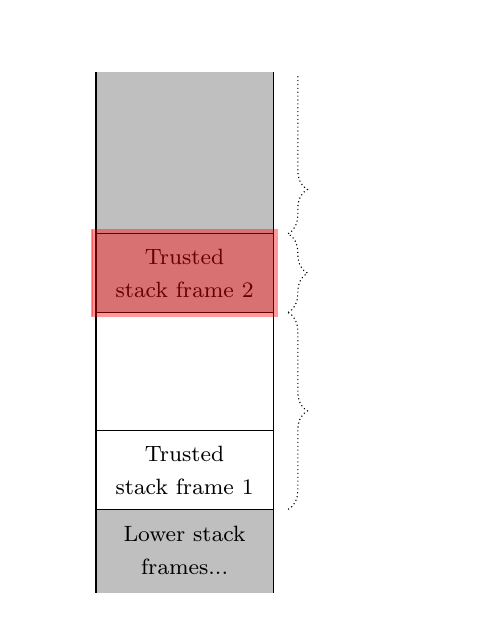
\begin{tikzpicture}[scale=.5, every node={scale=.5}]
      % recurrent parts
      \stdstackstart[13]
      \actsf{(0,2)}{(4.5,4)} {\footnotesize Trusted\\ \footnotesize stack frame 1}

      \inactsf{(0,7)}{(4.5,9)} {\footnotesize Trusted\\ \footnotesize stack frame 2}
      \begin{scope}
        \clip (-.1,-.1) rectangle (4.6,13.1);
        \draw[fill=gray!50] (0,9) rectangle (4.5,13.5);
      \end{scope}

      \lincapbrace{(4.6,2)}{(4.6,7)}{}

      \sealsymb{(4.9,8)}
      \lincapbrace{(4.6,7)}{(4.6,9)}{}

      \fill[red,draw=red,opacity=.4] (-.1,6.9) rectangle (4.6,9.1);
      \begin{scope}
        \clip (4.8,1) rectangle (9,13);
        \lincapbracebot{(4.6,9)}{(4.6,13.5)}{}
      \end{scope}

    \end{tikzpicture}
    \caption{}
    \label{fig:stack-base-abuse-d}
  \end{subfigure}
  \caption{Partial return token used to return out of order.}
  \label{fig:stk-base-abuse}
\end{figure}

\begin{figure}[htb]
  \centering
{\small
\[
  \begin{array}{r >{$}p{5.1cm}<{$} r l}
\multicolumn{2}{l}{\text{// Ensure non-empty stack.}}            & \multicolumn{2}{l}{\text{// Clear tmp registers and jump.}}\\
1 :& \tmove{\rtmp{1}}{42}                                        &14: & \tmove{\rtmp{1}}{0}\\
2 :& \tstore{\rstk}{\rtmp{1}}                                    &15: & \txjmp{r_1}{r_2}\\
3 :& \tcca{\rstk}{(-1)}                                          &\multicolumn{2}{l}{\text{// The following is the return code.}}\\
\multicolumn{2}{l}{\text{// Split stack in local stack frame and unused.}}      &\multicolumn{2}{l}{\text{// Check that returned stack pointer has base $\stkb$.}}\\
4 :& \tgeta{\rtmp{1}}{\rstk}                                     &16: & \tgetb{\rtmp{1}}{\rstk}\\
5 :& \tsplit{\rstk}{\rretd}{\rstk}{\rtmp{1}}                     &17: & \tminus{\rtmp{1}}{\rtmp{1}}{\stkb}\\
\multicolumn{2}{l}{\text{// Load the call seal.}}                &18: & \tmove{\rtmp{2}}{\pcreg}\\
6 :& \tmove{\rtmp{1}}{\pcreg}                                    &19: & \tcca{\rtmp{2}}{5}\\
7 :& \tcca{\rtmp{1}}{(\offpc - 5)}                               &20: & \tjnz{\rtmp{2}}{\rtmp{1}}\\
8 :& \tload{\rtmp{1}}{\rtmp{1}}                                  &21: & \rtmp{2}{1}\\
9 :& \tcca{\rtmp{1}}{\offsigma}                                  &22: & \tjmp{\rtmp{2}}\\
\multicolumn{2}{l}{\text{// Seal the local stack frame.}}        &23: & \tfail \\
10:& \tcseal{\rretd}{\rtmp{1}}                                   &\multicolumn{2}{l}{\text{// Splice with capability for local stack frame.}}\\
\multicolumn{2}{l}{\text{// Construct code return pointer.}}     &24: & \tsplice{\rstk}{\rstk}{\rdata} \\
11:& \tmove{\rretc}{\pcreg}                                      &\multicolumn{2}{l}{\text{// Pop 42 from the stack}}\\  
12:& \tcca{\rretc}{5}                                            &25: & \tcca{\rstk}{1}\\
13:& \tcseal{\rretc}{\rtmp{1}}                                   &\multicolumn{2}{l}{\text{// Clear tmp register}}\\
      &    &26: & \tmove{\rtmp{2}}{0}\\
  \end{array}
\]
}
\caption{
  % The instructions that constitutes a call. Register $r_1$ and $r_2$ are the registers where the sealed capability pair to the callee resides.
  % Variable $\offpc$ is the offset from the first instruction of the call to the set of seals, and $\offsigma$ is the offset to the seal within the set.
  % Instructions 1-3: ensure that the stack is non-empty.
  % Instructions 4-5: split stack pointer in two (stack pointer for callee done).
  % Instructions 6-9: Load the seal designated for this call.
  % Instruction 10: Seal capability for private stack to create data return pointer.
  % Instructions 11-13: Seal capability for return point to create code return pointer.
  % Instructions 14-15: Clean up temporary register and jump.
  % Instructions 16-26: The return code.
  % Instructions 16-23: check the stack base.
  % Instruction 24: join the stack pointer.
  % Instructions 25-26: pop 42 from the stack.
  The instructions for a $\scall{\offpc,\offsigma}{r_1}{r_2}$ with $\offpc$  the offset from line 1 of the call to the set of seals it uses and $\offsigma$ the offset in the set of seals to the call seal.
  $\stkb$ is the globally agreed on stack base.
  There are some magic numbers in the code: line 1: $42$, garbage data to ensure a non-empty stack.
  Line 7: $-5$, offset from line 6 (where $\pcreg$ was copied into $\rtmp{1}$) to line 1.
  Line 12: $5$, offset to the return address.
  Line 19: $5$, offset to fail.
  Line 21: offset to address after fail.
}
  \label{fig:call-code}
\end{figure}


% \begin{itemize}
% \item informally explain how an adversary may try to abuse stack and return caps
% \item informally explain how we prevent this using linear capabilities
% \item use the tikz pictures from the PriSC presentation to explain all of this
% \end{itemize}

\section{Formulating Security with a Fully Abstract Overlay Semantics}
\label{sec:form-secur-with}
As mentioned, the \stktokens{} calling convention guarantees well-bracketed control flow (WBCF) and local state encapsulation (LSE).
However, before we can prove these properties, we need to know how to even formulate them.
Although the properties are intuitively clear and sound precise, formalizing them is actually far from obvious.

Ideally, we would like to define the properties in a way that is
\begin{enumerate}
\item {\itshape intuitive} \label{def-prop:intuitive}
\item {\itshape useful for reasoning:} we should be able to use WBCF and LSE when reasoning about correctness and security of programs using \stktokens{}. \label{def-prop:useful}
\item {\itshape reusable in secure compiler chains:} for compilers using \stktokens{}, one should be able to rely on WBCF and LSE when proving correctness and security of other compiler passes and then compose such results with ours to obtain results about the full compiler.\label{def-prop:reusable}
\item {\itshape arguably "complete"}: the formalization should arguably capture the entire meaning of WBCF and LSE and should arguably be applicable to any reasonable program. \label{def-prop:complete}
\item {\itshape potentially scalable}: although dynamic code generation and multi-threading are currently out of scope, the formalization should, at least potentially, extend to such settings.\label{def-prop:scalable}
\end{enumerate}

Previous formalisations in the literature are formulated in terms of a static control flow graph~\cite[e.g., ][]{Abadi2005Theory}.
While these are intuitively appealing (\ref{def-prop:intuitive}), it is not clear how they can be used to reason about programs (\ref{def-prop:useful}) or other compiler passes (\ref{def-prop:reusable}), they lack temporal safety guarantees (\ref{def-prop:complete}) and do not scale (\ref{def-prop:scalable}) to settings with dynamic code generation (where a static control flow graph cannot be defined).
\citet{skorstengaard_reasoning_2017} provide a logical relation that
can be used to reason about programs using their calling convention
(\ref{def-prop:useful},\ref{def-prop:reusable}), but it is not intuitive (\ref{def-prop:intuitive}), there is no argument for completeness (\ref{def-prop:complete}), and it is unclear whether it will scale to more complex features (\ref{def-prop:scalable}).

We contribute a new way to formalise the properties using a novel approach we call fully abstract overlay semantics.
The idea is to define a second operational semantics for programs in our target language.
This second semantics uses a different abstract machine and different run-time values, but it executes in lock-step with the original semantics and there is a very close correspondence between the state of both machines.

The main difference between the two semantics, is that the new one satisfies LSE and WBCF by construction: the abstract machine comes with a built-in stack, inactive stack frames are unaddressable and well-bracketed control flow is built-in to the abstract machine.
Important run-time values like return capabilities and stack pointers are represented by special syntactic tokens that interact with the abstract machine's stack, but during execution, there remains a close, structural correspondence to the actual regular capabilities that they represent.
For example, stack capabilities in the overlay semantics correspond directly to linear capabilities in the underlying semantics, and they have authority over the part of memory that the overlay views as the stack.
\begin{jversion}
The new run-time values in the overlay semantics affect the definition of the encoding function $\encType{}$.
All the new values correspond to concrete capabilities on the \trgcm{} machine which the encoding function must respect.
For instance, the encoding of a stack pointer in the overlay semantics should be the same as the encoding of a linear capability on the \trgcm{} machine.
\end{jversion}

The fact that \stktokens{} enforces LSE and WBCF is then formulated as a theorem about the function that maps components in the well-behaved overlay semantics to the underlying components in the regular semantics.
The theorem states that this function constitutes a fully abstract compiler, a well-known property from the field of secure compilation~\cite{abadi_protection_1999}.
Intuitively, the theorem states that if a trusted component interacts with (potentially malicious) components in the regular semantics, then these components have no more expressive power than components which the trusted component interacts with in the well-behaved overlay semantics.
In other words, they cannot do anything that doesn't correspond to something that a well-behaved component, respecting LSE and WBCF, can also do.
More formally, our full-abstraction result states that two trusted components are indistinguishable to arbitrary other components in the regular semantics iff they are indistinguishable to arbitrary other components in the overlay semantics.

Our formal results are complicated by the fact that they only hold on a sane initial configuration of the system and for well-behaved components that respect the basic rules of the calling convention.
For example, the system should be set up such that seals used by components for constructing return pointers are not shared with other components.
We envision distributing seals as a job for the linker, so this means our results depend on the linker to do this properly.
As another example, a seal used to construct a return pointer can be reused but only to construct return pointers for the same return point.
Different seals must be used for different return points.
Such seals should also never be passed to other components.
These requirements are easy to satisfy: components should request sufficient seals from the linker, use a different one for every place in the code where they make a call to another component, and make sure to clear them from registers before every call.
The general pattern is that $\stktokens{}$ only protects components that do not shoot themselves in the foot by violating a few basic rules.
In this section, we define a well-formedness judgement for the syntactic requirements on components as well as a reasonability condition that semantically disallows components to do certain unsafe things.
Well-formedness is a requirement for all components (trusted and untrusted), but the reasonability requirement only applies to trusted components, i.e.\ those components for which we provide LSE and WBCF guarantees.

\begin{figure}[b]
  \centering
  \[
    \arraycolsep=1.4pt
    \begin{array}{rcl}
      \src{\SealableCaps} & \defbnf& \SealableCaps \mid \src{\stkptr{\permbnf,\basebnf,\aendbnf,\addrbnf}} \mid\\
                          & &   \src{\retptrd(\basebnf,\aendbnf)} \mid \src{\retptrc(\basebnf,\aendbnf,\addrbnf)}\\
      \multicolumn{3}{c}{
      \begin{array}{lcrclcr}
        \src{\StkFrame} & \defeq & \src{\Addr \times \MemSeg} & \phantom{skipskipsip} & \src{\Stack} & \defeq & \src{ \StkFrame^*}
      \end{array}
                                                                                                                }\\
      \src{\ExecConf} & \defeq & \Mem \times \Reg \; \src{\times \; \Stack \times \MemSeg} \\
    \end{array}
  \] 
\[
  \begin{array}{rclcrcl}
    \src{\Instr} & \defbnf &  \Instr \mid \scall{\offpc,\offsigma}{r}{r}&\phantom{skipskipskip}&
    \offpc,\offsigma & \in & \nats
  \end{array}
\]
\caption{The syntax of \srccm{}.
  \srccm{} extends \trgcm{} by adding stack pointers, return pointers, and a built-in stack.
  Everything specific to the overlay semantics is written in blue.
}
  \label{fig:source-syntax}
\end{figure}

% Update: see e-mail discussion: we do not see a good way to implement this.
% Dominique: I think it would be less confusing and more in line with the overlay semantics story to not add an extra instruction in Figure~\ref{fig:source-syntax} but rather present it as just a special case of the overlay semantics for the same underlying instructions.

\subsection{Overlay Semantics}
\label{subsec:overlay-semantics}
% Describe the things added to the syntax
The overlay semantics \srccm{} for \trgcm{} views part of the memory as a built-in stack (Figure~\ref{fig:source-syntax}).
% Built-in stack
To this end, it adds a call stack and a free stack memory to the executable configurations of \trgcm{}.
The call stack is a list with all the stack frames that are currently inaccessible because they belong to previous calls.
Every stack frame contains encapsulated stack memory as well as the program point that execution is supposed to return to.
The free stack memory is the active part of the stack that has not been claimed by a call and thus can be used at this point of time.
% Stack pointer
In order to distinguish capabilities for the stack from the capabilities for the rest of the memory, \srccm{} adds stack pointers.
A stack pointer has a permission, range of authority, and current address, just like capabilities on \trgcm{}, but they are always linear.
% Return pointers
The final syntactic constructs added by \srccm{} are the code and data return pointers.
The data return pointer corresponds to some stack pointer (which in turn corresponds to a linear capability), and the code return pointer corresponds to some capability with read-execute permission.
Syntactically, the return capabilities contain just enough information to reconstruct what they correspond to on the underlying machine.
On \srccm{}, return pointers are generated by calls from the capabilities they correspond to on \trgcm{}, and they are turned back to the capabilities they correspond to upon return.
% Even though the return pointers both correspond to capabilities with read permission, neither can be used for reading. 
% Say, we allowed reads through a data return pointer, then that would correspond to reading from some stack memory that is encapsulated in a stack frame which would break LSE.

The opaque nature of the return pointers is reflected in the interpretation of the instructions common to both \trgcm{} and \srccm{} as \srccm{} does not add special interpretation for them in non-\texttt{xjmp} instructions.
Stack pointers, on the other hand, need to behave just like capabilities, so \srccm{} adds new cases for them in the semantics, e.g.\ \texttt{cca} can now also change the current address of a stack pointer as displayed in Figure~\ref{fig:source-op-sem}.
Similarly, \texttt{load} and \texttt{store} work on the free part of the stack when provided with a stack pointer.
A store attempted with a stack capability that points to an address outside the free stack results in the $\failed$ configuration because that action is inconsistent with the view the overlay semantics has on the underlying machine.
In other words, there should only be stack pointers for the stack memory.

% Back to high-level view
As discussed earlier, our formal results only provide guarantees for components that respect the calling convention.
Untrusted components are not assumed to do so.
To formalize this distinction, \srccm{} has a set of trusted addresses $\ta$.
Only instructions at these addresses can be interpreted as the \srccm{} native call and push frames to the call stack which guarantees LSE and WBCF.
The constant $\ta$ is a parameter of the \srccm{} step relation.
Similarly, \stktokens{} assumes a fixed base address of the stack memory, that is also passed around as such a parameter, for use in the native semantics of calls.

Apart from the step relation of \trgcm{}, \srccm{} has one overlay step that takes precedence over the others.
This step is shown in Figure~\ref{fig:source-op-sem}, and it is different from the others in the sense that it interprets a sequence of instructions rather than one.
The sequence of instructions have to correspond to a call, i.e.\ the
instructions in Figure~\ref{fig:call-code} ({\footnotesize  $\scall[i]{\offpc,\offsigma}{r_1}{r_2}$} corresponds to the $i$'th instruction in the figure and $\calllen$ is always $26$, i.e.\ the number of instructions).
Calls are only executed when the well-behaved component executes, so the addresses where the call resides must be in $\ta$, and the executing capability must have the authority to execute the call.

% Call/return
The interpretation of $\scall{\offpc,\offsigma}{r_1}{r_2}$ is also shown in Figure~\ref{fig:source-op-sem} and essentially does the following:
The registers $r_1$ and $r_2$ are expected to contain a code-data pair sealed with the same seal and the unsealed values are invoked by placing them in the $\pcreg$ and $\rdata$ registers, respectively.
The current active stack and the stack capability are split into the local stack frame of the caller and the rest.
$\scall{}{}{}$ also constructs a return capability $c_{\var{opc}}$ and its address $\var{opc}$, pointing after the call instructions.
The local stack frame and return address are pushed onto the stack, and the local stack capability and return capability are converted into a pair of sealed return capabilities.
The return capabilities are sealed with the seal designated for the call.

The return capabilities, $\retptrc$ and $\retptrd$ are sealed and can only be used using the \texttt{xjmp} instruction, to perform a return.
When this happens, the topmost call stack frame $(\opc,\ms_\var{local})$ is popped from the call stack.
In order for the return to succeed, the return address in the code return pointer must match $\opc$, and the range of addresses in the data return pointer must match the domain of the local stack.
If the return succeeds, the stack pointer is reconstructed, and the local stack becomes part of the active stack again.

\srccm{} supports tail calls.
A tail call is a call from a caller that is done executing, and thus doesn't need to be returned to or preserve local state.
This means that a tail call should not reserve a slot in the return order by pushing a stack frame on the call stack, i.e.\ it should not use the built-in call.
To perform a tail call, the caller simply transfers control to the callee using \texttt{xjmp}.
The tail-callee should return to the caller's caller, so the caller leaves the return pair they received for the callee to use.

It is important to observe that the operational semantics of \srccm{} natively guarantee WBCF (well-bracketed control flow) and (local stack encapsulation) for calls made by trusted components.
By inspecting the operational semantics of \srccm{}, we can see that it never allow reads or writes to inactive stack frames on the call stack.
The built-in call for trusted code pushes the local stack frame to the inactive part of the stack, together with the return address. 
Such frames can be reactivated by \texttt{xjmp}ing to a return capability pair, but only for the topmost stack frame and if the return address corresponds to the one stored in the call stack.
In other words, WBCF and LSE are natively enforced in this semantics.

\begin{figure}[htb]
  \centering
  \begin{mathpar}
    \inferrule{\src{\Phi(\pcreg) = ((\perm,\_),\baddr,\eaddr,\aaddr)} \\
               \src{\lbrack \aaddr ,\aaddr + \calllen - 1\rbrack \subseteq \ta}  \\
               \src{\lbrack\aaddr,\aaddr + \calllen-1\rbrack \subseteq [\baddr,\eaddr]} \\
               \src{\perm \in \{\rwx,\rx\}} \\
               \src{\Phi.\mem(\aaddr,\dots,\addr + \calllen-1) = \scall[0]{\offpc,\offsigma}{r_1}{r_2} \cdots \scall[\calllen-1]{\offpc,\offsigma}{r_1}{r_2}}
 }
              { \src{\Phi}  \; \src{\step[\src{\ta,\stkb}] \sem{\scall{\offpc,\offsigma}{r_1}{r_2}}(\Phi)} }
  \end{mathpar}
  \begin{tabular}{|>{$}c<{$}|p{3.7cm}|>{\raggedright\arraybackslash}p{6.6cm}|}
    \hline
    i \in \src{\Instr}                                 & $\sem{i}(\Phi)$ & Conditions\\
    \hline
    \halt                                        & $\halted$ & \\
    \hline
    \multicolumn{3}{|c|}{\dots\text{ (the operational semantics of \trgcm)}} \\
    \hline
    \store{r_1}{r_2}                             & $\srcalt{\var{updPc}} \sourcecolor\arraycolsep=0pt\array[t]{rl}(\Phi&\updReg{r_2}{w_2}\\ &\update{\ms_\stk.\aaddr}{\Phi(r_2)})\endarray$  & \srcalt{$\Phi(r_1) = \stkptr{\perm,\baddr,\eaddr,\aaddr}$ and $\perm \in \{\rwx,\rw\}$ and $\baddr \le \aaddr \le \eaddr$ and $w_2 = \linCons{\Phi(r_2)}$ and $\aaddr \in \dom(\ms_\stk)$}\\
    \hline
    \cca{r}{\rn}                                 &$\srcalt{\updPcAddr{\Phi\updReg{r}{w}}}$ &  \srcalt{$\Phi(\rn) = n \in \ints$ and $\Phi(r) = \stkptr{\perm,\baddr,\eaddr,\aaddr}$ and $w = \stkptr{\perm,\baddr,\eaddr,\aaddr+n}$} \\
    \hline
    \arraycolsep=0pt\array{c}
    \scall{\srcalt{\offpc,\offsigma}}{\src{r_1}}{\src{r_2}}
    \endarray &
        $\srcalt{\var{xjmpRes}(c_1,c_2,}$
        $\srcalt{\hspace{.25cm}\left(\arraycolsep=0pt\array[c]{rl}\Phi&\updReg{r_1,r_2}{w_1,w_2}\\
            &\updReg{\rretc}{s_c}\\
            &\updReg{\rretd}{s_d}\\
            &\updReg{\rstk}{c_\stk}\\
            &\update{\ms_\stk}{\ms_{\stk,\var{rest}}}\\
            &\update{\stk}{\stk'}\\
            \endarray\right))}$
       &
      \srcalt{
         $\begin{multlined}
           \ms_{\stk,\var{local}},c_\var{local},\ms_{\stk,\var{rest}},c_\stk =\\ \var{splitStack}(\Phi.\reg(\rstk), \Phi.\ms_\stk) \text{ and }
         \end{multlined}$
    $\opc, c_\opc =\var{setupOpc(\Phi.\reg(\pcreg))}$ and
    $\stk' = (\opc,\ms_{\stk,\var{local}}) :: \Phi.\stk$ and 
    $\sigma =\begin{multlined}[t]
      \var{getCallSeal}(\\
      \Phi.\reg(\pcreg), \Phi.\mem,\offpc,\offsigma)  \text{ and }
    \end{multlined}$
    $s_c,s_d = \var{sealReturnPair}(\sigma,c_\opc,c_\var{local})$ and
    $w_1,w_2 = \linCons{\Phi.\reg(r_1,r_2)}$ and
                        $\Phi.\reg(r_1,r_2) = \sealed{\sigma', c_1}, \sealed{\sigma', c_2}$
                        }\\
    \hline 
    \multicolumn{3}{|c|}{\dots} \\
    \hline
    \_                                           & $\failed$ & \totherwise \\
    \hline
  \end{tabular}
\begin{multline*}
  \srcxjmpres{c_1,c_2,\Phi} = \\
  \left\{ 
    \arraycolsep=1.4pt
    \begin{array}{l c >{\raggedright\arraybackslash}p{9.5cm}}
      \arraycolsep=0pt
    \begin{array}{rl}
      \Phi & \updReg{\pcreg}{c_1}\\
           & \updReg{\rdata}{c_2}
    \end{array}
    &\phantom{mak} & $\nonExec{c_2}$ \srcalt{and $c_1 \neq \retptrc(\_)$ and $c_2 \neq \retptrd(\_)$}\\
      \arraycolsep=0pt
      \array[c]{rl}
      \Phi&\updReg{\pcreg}{c_\opc}\\
          &\updReg{\rstk}{c_\stk}\\
          &\updReg{\rdata}{0}\\
          &\update{\stk}{\stk'}\\
          &\update{\ms_\stk}{\ms_\stk \uplus \ms_\var{local}}
      \endarray
           & &
               $\arraycolsep=0pt\array{l}
        \src{(\opc, \ms_\var{local}) :: \stk'= \Phi.\stk \tand} \\
      \src{c_1 = \retptrc(\baddr,\eaddr,\opc)}\\
      \src{c_2 = \retptrd(\aaddr_\stk,\eaddr_\stk) \wedge \dom(\ms_\var{local}) = [\aaddr_\stk,\eaddr_\stk]}\\
      \src{c_\stk = \var{reconstructStackPointer}(\Phi.\reg(\rstk),c_2) \tand}\\
      \src{c_\opc =  ((\rx,\normal),\baddr,\eaddr,\opc)} 
      \endarray$\\
      \failed &  & \totherwise
    \end{array} 
\right.
\end{multline*}
  \caption{An excerpt of the operational semantics of \srccm{} (some details omitted). Auxiliary definitions are found in Figure~\ref{fig:source-op-sem-aux}. }
  \label{fig:source-op-sem}
\end{figure}


\begin{figure}
    \begin{multline*}
      \src{\var{splitStack}(\stkptr{\rw,\baddr_\stk,\eaddr_\stk,\aaddr_\stk}, \ms_\stk) = \ms_{\stk,\var{local}},c_\var{local\_data},\ms_{\stk,\var{unused}},c_\stk} \mathit{\ iff\ } \\
      \left\{ 
      \begin{array}{l}
      \src{\baddr_\stk < \aaddr_\stk \leq \eaddr_\stk }\\
      \src{\ms_{\stk,\var{local}} = \ms_\stk |_{[\aaddr_\stk,\eaddr_\stk]}\update{\aaddr_\stk}{42} }\\
      \src{\ms_{\stk,\var{unused}} = \ms_\stk|_{[\baddr_\stk,\aaddr_\stk-1]} }\\
      \src{c_\stk = \stkptr{\rw,\baddr_\stk,\aaddr_\stk-1,\aaddr_\stk-1} }\\
      \src{c_\var{local\_data} = \retptrd(\aaddr_\stk,\eaddr_\stk) }\\
      \end{array}
      \right.
    \end{multline*}
    \begin{align*}
      \src{ \var{setupOpc(((\_,\_),\baddr,\eaddr,\aaddr))}} &\ \src{= \opc, c_\opc} \mathit{\ iff\ }
      \left\{ 
      \begin{array}{l}
      \src{\opc = \aaddr + \calllen \wedge{}}\\
      \src{c_\opc = \retptrc(\baddr,\eaddr,\opc) \wedge{}}
      \end{array}
       \right.\\
      \src{\var{getCallSeal}(c_\pcreg,\mem,\offpc,\offsigma)} &\ \src{= \sigma} \mathit{\ iff\ }
      \left\{
      \begin{array}{l} 
      \src{c_\pcreg = ((\_,\_),\baddr,\eaddr,\aaddr) \wedge \baddr \leq  \aaddr+\offpc \leq \eaddr \wedge{}} \\
      \src{\mem(\aaddr+\offpc) = \seal{\sigma_\baddr,\sigma_\eaddr,\sigma_\aaddr} \wedge{} \sigma_\baddr \leq \sigma \leq \sigma_\eaddr \wedge{}}\\
      \src{\sigma = \sigma_\aaddr + \offsigma }
      \end{array}
      \right.\\
     \src{\var{sealReturnPair}(\sigma,c_\opc,c_\var{local})} &\ \src{= \sealed{\sigma,c_\opc},\sealed{\sigma,c_\var{local}}}
    \end{align*}%
  % \begin{multline*}
  %   \src{\var{callConditions}(r_1,r_2,\offpc,\offsigma,(\mem,\reg,\stk,\ms_\stk)) = (\mem,\reg',\stk',\ms_{\stk,\var{rest}})}\mathit{\ iff}\\
  %     \quad\quad\left\{ 
  %       \begin{array}{l}
  %         \src{\var{sealedPairArgument}(\reg,r_1,r_2,c_1,c_2)}\\
  %     \src{\ms_{\stk,\var{local}},\ms_{\stk,\var{rest}},c_\stk,c_\var{local\_data} = \var{splitStack}(\reg, \ms_\stk) \wedge{}}\\
  %     \src{\opc, c_\opc =\var{setupOpc(\reg)} \wedge{}}\\
  %     \src{\stk' = (\opc,\ms_{\stk,\var{local}}) :: \stk \wedge{}}\\
  %     \src{\sigma = \var{getCallSeal}(\reg,\mem,\offpc,\offsigma) \wedge{}}\\
  %     \src{s_c,s_d = \var{sealReturnPair}(\sigma,c_\var{local\_data},c_\opc) \wedge{}}\\
  %     \src{w_1,w_2 = \linCons{\reg(r_1),\reg(r_2)} \wedge{}}\\ 
  %     \src{\reg' =\reg\updReg{r_1,r_2}{w_1,w_2}\updReg{\rretc,\rretd}{s_c,s_d}\updReg{\rstk,\rtmp{1}}{c_\stk,0}}
  %     \end{array}\right.
  % \end{multline*}
  \begin{multline*}
    \src{\var{reconstructStackPointer}(\stkptr{\rw, \stkb, \aaddr_\stk-1,\_},\retptrd(\aaddr_\stk,\eaddr_\stk)) =}\\ \src{\stkptr{\rw,\stkb,\eaddr_\stk,\aaddr_\stk}} \mathit{\ iff\ }
        \src{\stkb \leq \addr_\stk }
   \end{multline*}

  \caption{Auxiliary definitions used in the operational semantics of \srccm{}.}
  \label{fig:source-op-sem-aux}
\end{figure}
% \begin{figure}
% % \[
% %     \src{\stkptr{\rw,\stkb,\eaddr_\stk,\aaddr_\stk} = \var{tokenToStkPtr}(\retptrd(\aaddr_\stk,\eaddr_\stk)}
% % \]
% % \[
% %     \src{\stk', \ms_\var{local\_stk} = \var{popCallStackFrame} (\stk,c_1,c_2)}
% %     \mathit{\ iff\ }
% %       \left\{ \array{l}
% %         \src{\stk = (\opc, \ms_\var{local\_stk}) :: \stk' \wedge{}} \\
% %         \src{c_1 = \retptrc(\_,\_,\opc) \wedge{}} \\
% %         \src{c_2 = \retptrd(\aaddr_\stk,\eaddr_\stk)\wedge{}} \\
% %         \src{\dom(\ms_\var{local\_stk}) \subseteq [\aaddr_\stk,\eaddr_\stk]}
% %         \endarray
% %      \right.
% % \]
% % \[
% %   \src{\var{retPtrForMatchLocalStack(\retptrd(\aaddr_\stk,\eaddr_\stk),\ms_\var{local})}} \mathit{\ iff\ } \src{\dom(\ms_\var{local} \subseteq [\aaddr_\stk,\eaddr_\stk])}
% % \]

% % \begin{multline*}
% %     \src{(\mem,\reg',\stk',\ms_\stk') = \var{returnCondition}(c_1,c_2,(\mem,\reg,\stk,\ms_\stk))}\mathit{\ iff\ }\\
% %       \quad\quad\left\{ 
% %       \begin{array}{l}
% %       \src{\stk', \ms_\var{local\_stk} = \var{popCallStackFrame}(\stk,c_1,c_2)}\\
% %       \src{c_\stk = \var{reconstructStackPointer}(\reg,c_2)}\\
% %       \src{c_\opc =  \var{tokenToPc}(c_1)} \\
% %       \src{\ms_\stk' = \ms_\stk \uplus \ms_\var{local\_stk}} \\
% %       \src{\reg' =\reg\updReg{\pcreg,\rstk}{c_\opc,c_\stk}\updReg{\rdata,\rtmp{1},\rtmp{2}}{0,0,0}}
% %       \end{array}\right.
% %   \end{multline*}

%   \caption{The return condition in the operational semantics of \srccm{}.}
%   \label{fig:source-op-sem-return}
% \end{figure}
\subsection{Well-Formed Components}
\label{sec:well-form-reas}
% Well-formed components
% \begin{figure}[htb]
%   \centering
%   \begin{mathpar}
%   \inference{
%     \dom(\mscode) = [\baddr,\eaddr]&
%     [\baddr-1,\eaddr+1] \mathrel{\#} \dom(\msdata)\\
%     \mspad = [\baddr-1\mapsto 0] \uplus [\eaddr+1 \mapsto 0]\\
%     \sigrets,\sigcloss \vdash_{\mathrm{comp-code}} \mscode \\
%     \exists A_\mathrm{own} : \dom(\msdata) \rightarrow \powerset{\dom(\msdata)} & \dom(\msdata) = A_{\mathrm{non-linear}} \uplus A_\linear \\
%     A_\linear = \biguplus_{a \in \dom(\msdata)} A_{\mathrm{own}}(a) \\
%     \forall a \in \dom(\msdata)\ldotp \dom(\mscode),A_{\mathrm{own}}(a),A_{\mathrm{non-linear}},\sigrets,\sigcloss \vdash_{\mathrm{comp-value}} \msdata(a)\\
%     \overline{\var{export}} = \overline{s_{\mathrm{export}} \mapsto w_{\mathrm{export}}} & \overline{\var{import}} = \overline{a_{\mathrm{import}} \mapsfrom s_{\mathrm{import}}}& \{\overline{a_{\mathrm{import}}}\} \subseteq \dom(\msdata)\\
%     \overline{\dom(\mscode), A_{\mathrm{non-linear}}, \sigrets,\sigcloss \vdash_{\mathrm{comp-export}} w_{\mathrm{export}}}\\
%     \overline{s_{\mathrm{import}}} \mathrel{\#} \overline{s_{\mathrm{export}}} & (\dom(\mscode) \subseteq \ta) \vee (\dom(\mscode) \mathrel{\#} \ta \wedge \sigrets = \emptyset)&
%     \dom(\msdata) \mathrel{\#} \ta
%   }{
%     \vdash (\mscode\uplus \mspad,\msdata,\overline{\var{import}},\overline{\var{export}},\sigrets,\sigcloss,A_\linear)
%   }
%   \and
%   \inference{
%     \comp_0 = (\mscode,\msdata,\overline{\var{import}},\overline{\var{export}},\sigrets,\sigcloss,A_\linear)\\
%     \vdash \comp_0 & (\_ \mapsto c_{\mathrm{main},c}), (\_ \mapsto c_{\mathrm{main},d}) \in \overline{\var{export}}
%   }{
%     \vdash (\comp_0,c_{\mathrm{main},c}, c_{\mathrm{main},d})
%   }
% \end{mathpar}
%   \caption{Exceprt of well-formedness judgement}
%   \label{fig:well-formedness}
% \end{figure}
% Well-formedness highlights:
% Main exported
% Code memory:
% - Only instructions and seals
% - calls associated with return seals unique return seal
% - only uses seals specified for components
% - (No linear access)
% Data memory:
% - Data
% - Capabilities fora data memory (linearity respected)
% - Sealed caps sealed with clos seal
% Exports
% - Any Word valid in data memory or
% - Sealed capability for code (sealed with clos seal)
% Imports
% - Address must be in data memory
\begin{jversion}
  The components introduced in Section~\ref{subsec:components-linking} are pretty much unconstrained.
  For instance, a component can have multiple linear capabilities for the same piece of memory, and there are no restrictions on seals.
  In a real system, the operating system and linker  % ???
  would make sure everything is setup correctly.
  For instance, they would not allocate multiple linear capabilities for the same memory, and they would ensure sane seal allocation.

  The component notion is used for both trusted and adversarial components.
  We expect the linker to link the two programs together making sure that all the system invariants are respected.
  We expect trusted components to be the product of a known compiler that uses \stktokens{} which means that the code must have a certain shape.
  The proper linker behaviour and the syntactic expectations we have of trusted component are captured in a syntactic well-formedness judgement which we explain in this section.

  The well-formedness judgement imposes a quite rigid structure on well-formed components: a component's code memory may contain only data and sets of seals.
  The data memory may contain only data, memory capabilities to the component's data memory (respecting linearity) or sealed memory capabilities (to the component's data memory, sealed with closure seals).
  This makes a clear separation between code and data memory as neither can contain capabilities for the other.
  The separation of the two kinds of memory means that data structures in data memory can be shared without risking unintentionally leaking a return seals that were indirectly accessible through the data structure.
  Informally, a well-formed component respects Write-XOR-Execute which means that all capabilities for code memory at most has read-execute permission and all capabilities for data memory at most has read-write permission.
  A component's exports should be sealed code or data capabilities, sealed with a closure seal.

  As discussed before, we only provide guarantees (LSE and WBCF) for components respecting certain semantic rules (reasonable use of seals).
  Components that do not satisfy these requirements are still allowed in \srccm{}, but (as we will see below) function calls in such components will not behave according to the special \srccm{} semantics that guarantees LSE and WBCF.
  To distinguish trusted components (which satisfy reasonability requirements) from adversarial components (which don't), we make use of a set of trusted addresses $\ta$.
  Any component's code memory must fall entirely within or outside of $\ta$, so every component is either trusted or adversarial.
  Some well-formedness requirements are specific for adversarial and trusted components.
  Well-formed adversarial components cannot have return seals.
  On the other hand, well-formed trusted components can have return seals, but must make return seals available to all its calls in a way that is consistent with \stktokens{}.
  This means that each return seal is only used for one call.
\end{jversion}

% We first highlight the main points of the $\wdjud[\ta]{\comp}$ judgement.
% For components with a main pair, the main pair must come from the exports and the remainder of the component must be well-formed.
% As a reminder, a base component looks like this: $(\mscode,\msdata,\overline{\var{import}},\overline{\var{export}},\sigrets,\sigcloss,A_\linear)$.
% The return seals $\sigrets$ are the seals supposed to be usedto seal return pointers and the closure seals $\sigcloss$ all the other seals in a component.
% If a component is adversarial, i.e.\ the domain of the code memory $\mscode$ is disjoint from the set of trusted addresses $\ta$, then there should be no return seals.
% The code memory may contain sets of seals but only for the seals in $\sigrets$ and $\sigcloss$.
% Other than that, code memory only contains instructions in the form of integers.
% When a sequence of instructions in the code memory corresponds to a call (Figure~\ref{fig:call-code}), the call must have access to the return seal it specifies.
% The return seal also needs to be unique to that call; that is, no other call can specify the same seal as its return seal.
% The data memory $\msdata$ may contain data, capabilities, and sealed capabilities.
% The capabilities in the data memory can only have authority over the data memory itself.
% This allows components to have initial data structures.
% In order to respect Write-XOR-Execute, the capabilities in data memory cannot have execute permission.
% The capabilities also need to respect linearity which means that linear capabilities cannot be aliased by any other capability, and they must be for a range of the predetermined linear addresses $A_\linear$.
% The sealed capabilities must be sealed with a closure seal, and the sealable can be anything that is allowed to reside in data memory.
% The exports $\overline{\var{export}}$ can be anything non-linear allowed to reside in data memory or a sealed capability for the code memory sealed with one of the closure seals.

\begin{figure}
\begin{mathpar}
  \inferrule*[Right=Base]{
    \dom(\mscode) = [\baddr,\eaddr]\\
    [\baddr-1,\eaddr+1] \mathrel{\#} \dom(\msdata)\\
    \mspad = [\baddr-1\mapsto 0] \uplus [\eaddr+1 \mapsto 0]\\
    \exists A_\mathrm{own} : \dom(\msdata) \rightarrow \powerset{\dom(\msdata)}\\
    \dom(\msdata) = A_{\mathrm{non-linear}} \uplus A_\linear \\
    A_\linear = \biguplus_{a \in \dom(\msdata)} A_{\mathrm{own}}(a) \\
    \overline{\var{export}} = \overline{s_{\mathrm{export}} \mapsto w_{\mathrm{export}}} \\
    \overline{\var{import}} = \overline{a_{\mathrm{import}} \mapsfrom s_{\mathrm{import}}} \\
    \{\overline{a_{\mathrm{import}}}\} \subseteq \dom(\msdata)\\
    \overline{s_{\mathrm{import}}} \mathrel{\#} \overline{s_{\mathrm{export}}} \\
    (\emptyset \neq \dom(\mscode) \subseteq \ta) \vee (\dom(\mscode) \mathrel{\#} \ta \wedge \sigrets = \emptyset) \\
    \dom(\msdata) \mathrel{\#} \ta \\
    \sigrets,\sigcloss,\ta \vdash_{\mathrm{comp-code}} \mscode \\
    \forall a \in \dom(\msdata)\ldotp \dom(\mscode),A_{\mathrm{own}}(a),A_{\mathrm{non-linear}},\sigcloss \vdash_{\mathrm{comp-word}} \msdata(a)\\
    \overline{\dom(\mscode), A_{\mathrm{non-linear}}, \sigrets,\sigcloss \vdash_{\mathrm{comp-export}} w_{\mathrm{export}}}
  }{
    \ta \vdash (\mscode\uplus \mspad,\msdata,\overline{\var{import}},\overline{\var{export}},\sigrets,\sigcloss,A_\linear)
  }
  \and
  \inferrule*[Right=Main]{
    \var{comp}_0 = (\mscode,\msdata,\overline{\var{import}},\overline{\var{export}},\sigrets,\sigcloss,A_\linear)\\
    \ta \vdash \var{comp}_0 \\
    (\_ \mapsto c_{\mathrm{main},c}), (\_ \mapsto c_{\mathrm{main},d}) \in \overline{\var{export}}
  }{
    \ta \vdash (\var{comp}_0,c_{\mathrm{main},c}, c_{\mathrm{main},d})
  }
\end{mathpar}
\caption{Well-formedness judgement.}
\label{fig:well-formed}
\end{figure}

\begin{jversion}
These requirements are formally expressed by the judgement $\wdjud[\ta]{\comp}$ specifies, i.e.\ it defines when components satisfy the initial syntactic requirements necessary to be able to rely on unique linear capabilities, component unique seals, etc.
The judgement is defined in \figurename~\ref{fig:well-formed} with auxiliary judgements in \figurename~\ref{fig:well-formed-aux}.

The $\wdjud[\ta]{\comp}$ judgement has two rules: \textsc{Main} and \textsc{Base}.
The \textsc{Main} rule requires the component to have an entry point in terms of a main pair from the exports.
Further, the base component should satisfy the well-formedness judgement.
The \textsc{Base} judgement ensures sure that the component has a bit of structure.
Roughly speaking, the \textsc{Base} rule requires the following:
\begin{itemize}
\item \textit{Code and data memory are disjoint.}
\item \textit{Code memory is padded with zeros ($\mspad$).}
  This prevents code memories from being spliced together.
  If the capabilities for two code memories can be spliced together, then the execution of one code memory can continue into the other creating an unintended control-flow.
  Further, the possible control-flows of a component suddenly depends on the memory locations of all the components\footnote{Alternatively to this syntactic condition on components, we could require trusted components to never splice executable capabilities of unknown origin.}.
\item \textit{All memory can either be addressed by any number of non-linear capabilities or at most one linear capability.}
  The data address space is split into $A_\var{non-linear}$ and $A_\var{linear}$ that can be addressed by non-linear capabilities and linear capabilities, respectively.
  The judgement ensure uniqueness of linear capabilities by letting each address of the data memory take sole ownership of addresses in $A_\var{linear}$.
\item \textit{All import addresses are part of the data memory.} 
\item \textit{Import and export symbols are disjoint.}
\item \textit{One of the following two are true}
  \begin{itemize}
  \item \textit{The code address space is disjoint from the trusted address space $\ta$ and there are no return seals.} In this case, the component contains untrusted code. We are interested in WBCF and LSE from the perspective of the trusted code, so we do not let untrusted memory have return seals\footnote{Untrusted code still has access to seals that could be used to protect calls.}.
  \item \textit{The code address space is part of the trusted address space $\ta$.} In this case, the component contains trusted code. We do not impose requirements on the return seals here (the auxiliary judgements will impose restrictions on them), so the trusted component can have the return seals necessary for its calls.
  \end{itemize}
\item \emph{The data address space is disjoint from the trusted address space $\ta$.} Data memory is not executable, so the trusted addresses never include the data memory addresses.
\item \textit{The code memory satisfies the component-code judgement (\figurename~\ref{fig:well-formed-code}).}
\item \textit{Each word in the data memory satisfies the component-word judgement (\figurename~\ref{fig:well-formed-word}).} This must be with respect to the linear addresses assigned to this address.
\item \textit{All the exports satisfy the components-export judgement (\figurename~\ref{fig:well-formed-export}).}
\end{itemize}

\begin{figure}
  \begin{subfigure}[h]{1.0\linewidth}
    \begin{mathpar}
  \inferrule*[Right=C-Seals]{
    \mscode(a) = \seal{\sigma_\baddr,\sigma_\eaddr,\sigma_\baddr} \\ [\sigma_\baddr,\sigma_\eaddr] = (\sigrets \cup \sigcloss)
  }{
    \sigrets,\sigrets[\mathrm{owned}],\sigcloss,\ta \vdash_{\mathrm{comp-code}} \mscode,a
  }
  \and
  \inferrule*[Right=C-Instr]{
    \mscode(a) \in \ints\\
{    \begin{multlined}
      ([a \cdots a + \calllen-1] \subseteq \ta \wedge \mscode([a \cdots a + \calllen-1]) = \scall[0..\calllen-1]{\offpc,\offsigma}{r_1}{r_2})
      \Rightarrow\\ (\mscode(a+\offpc) = \seal{\sigma_\baddr,\sigma_\eaddr,\sigma_\baddr} \wedge \sigma_\baddr+\offsigma \in \sigrets[\mathrm{owned}])
    \end{multlined}
}  }{
    \sigrets,\sigrets[\mathrm{owned}],\sigcloss,\ta \vdash_{\mathrm{comp-code}} \mscode,a
  }
  \and
  \inferrule*[Right=C-Mem]{
    \text{$\mscode$ has no hidden calls}\\
    \sigrets \mathrel{\#} \sigcloss \\
    \exists d_\sigma : \dom(\mscode) \rightarrow \powerset{\Seal} \ldotp
    \sigrets = \biguplus_{a \in \dom(\mscode)} d_\sigma(a) \tand\\
    \forall a \in \dom(\mscode) \ldotp 
    \sigrets,d_\sigma(a),\sigcloss,\ta \vdash_{\mathrm{comp-code}} \mscode,a\\
    \exists a \ldotp \mscode(a) = \seal{\sigma_\baddr,\sigma_\eaddr,\_} \wedge [\sigma_\baddr,\sigma_\eaddr] \neq \emptyset
  }{
    \sigrets,\sigcloss,\ta\vdash_{\mathrm{comp-code}} \mscode
  }
    \end{mathpar}
    \caption{Code well-formedness.}
    \label{fig:well-formed-code}
  \end{subfigure}
  
  \begin{subfigure}[h]{1.0\linewidth}
    \begin{mathpar}
      \inferrule*[Right=W-Data]{
        z \in \ints
  }{
    A_{\mathrm{code}},A_{\mathrm{own}},A_{\mathrm{non-linear}},\sigcloss \vdash_{\mathrm{comp-word}} z
  }
  \and
  \inferrule*[Right=W-Capability]{
    \permbnf \sqsubseteq \rw\\
    \lin = \linear \Rightarrow \emptyset \subset [\baddr,\eaddr] \subseteq A_{\mathrm{own}} \\\\
    \lin = \normal \Rightarrow [\baddr,\eaddr] \subseteq A_{\mathrm{non-linear}}
  }{
    A_{\mathrm{code}},A_{\mathrm{own}},A_{\mathrm{non-linear}},\sigcloss \vdash_{\mathrm{comp-word}} ((\perm,\lin),\baddr,\eaddr,\aaddr)
  }
  \and
  \inferrule*[Right=W-Sealed-Capability]{
    A_{\mathrm{code}},A_{\mathrm{own}},A_{\mathrm{non-linear}},\sigcloss \vdash_{\mathrm{comp-word}} \vsc \\
    \sigma \in \sigcloss
  }{
    A_{\mathrm{code}},A_{\mathrm{own}},A_{\mathrm{non-linear}},\sigcloss \vdash_{\mathrm{comp-word}} \sealed{\sigma,\vsc}
  }
    \end{mathpar}
    \caption{Word well-formedness.}
    \label{fig:well-formed-word}
  \end{subfigure}
  
  \begin{subfigure}[h]{1.0\linewidth}
    \begin{mathpar}
  \inferrule*[Right=E-Sealed-Code]{
    [\baddr,\eaddr] \subseteq A_{\mathrm{code}} \\
    \sigma \in \sigcloss
  }{
    A_{\mathrm{code}},A_{\mathrm{non-linear}},\sigcloss \vdash_{\mathrm{comp-export}} s \mapsto \sealed{\sigma,((\rx,\normal),\baddr,\eaddr,\aaddr)}
  }
  \and
  \inferrule*[Right=E-Word]{
    A_{\mathrm{code}},\emptyset,A_{\mathrm{non-linear}},\sigcloss \vdash_{\mathrm{comp-word}} w
  }{
    A_{\mathrm{code}},A_{\mathrm{non-linear}},\sigcloss \vdash_{\mathrm{comp-export}} s \mapsto w
  }
    \end{mathpar}
    \caption{Export well-formedness}
    \label{fig:well-formed-export}
  \end{subfigure}
  \caption{Well-formedness judgement for code, words, and export. $\calllen$ it the length of the call code.}
  \label{fig:well-formed-aux}
\end{figure}
\figurename~\ref{fig:well-formed-word} defines the judgement $\vdash_{\mathrm{comp-word}}$ which specifies the words that are well-formed in a component's data memory.
The judgement is defined by three rules: \textsc{W-Data}, \textsc{W-Capability}, and \textsc{W-Sealed-Capability}.
The \textsc{W-Data} rule says all data, i.e.\ integers, are well-formed words.
The \textsc{W-Capability} rule specifies that all well-formed capabilities in data memory must at most have read and write permission.
Further, if the capability is linear, then the range of authority must be within the linear address space owned by this address.
Finally, if it is non-linear, then it must be in the non-linear address space.
The \textsc{W-Sealed-Capability} specifies that well-formed sealed capabilities in data memory are sealed with a closure seal and whatever is sealed is itself a well-formed word.
Because of the last requirement, the data memory cannot initially contain sealed code capabilities.
However, a component is free to place sealed data capabilities in memory during execution.

\figurename~\ref{fig:well-formed-export} defines the well-formed exports $\vdash_{\mathrm{comp-export}}$.
\textsc{E-Word} says that any well-formed word for data memory is well-formed as an export.
In particular, this means that sealed capabilities for the data memory are acceptable exports which allows components to export the data part of a sealed capability pair.
The \textsc{E-Sealed-Code} rule allows the code part of a sealed capability pair to be exported.
In particular, it allows a capability with read-execute permission and its range of authority within the component's code address space to be exported when it has been sealed with a closure seal.
Together, these two rules allow components to export closures.

\figurename~\ref{fig:well-formed-code} defines the well-formed code memories $\vdash_{\mathrm{comp-code}}$.
The well-formed code memories are defined by two judgements.
One judgement considers the entire memory $\sigrets,\sigcloss,\ta\vdash_{\mathrm{comp-code}} \mscode$ while the other considers the contents of each code memory address $\sigrets,\sigrets[\mathrm{owned}],\sigcloss,\ta \vdash_{\mathrm{comp-code}} \mscode,a$.
Unlike data memory and exports, we cannot say whether code memory is well-formed by considering each word in isolation.
The well-formedness of code memory depends on whether seals for calls are located in the place we expect them to be located.
The $\sigrets,\sigrets[\mathrm{owned}],\sigcloss,\ta \vdash_{\mathrm{comp-code}} \mscode,a$ judgement has two rules.
The \textsc{C-Seal} judgement requires address $a$ in $\mscode$ to contain a set of seals that is a subset of the closure seals and the return seals.
\textsc{C-Instr} requires address $a$ to contain an integer, which may be interpreted as instruction.
If address $a$ is the first address of a series of instructions that may be interpreted as a call, and all the addresses are within the trusted address space, then there must be a set of seals available at the address the call in question expects it and that set of seals must contain the return seal that corresponds to the return seal of this call.
The return seal in question must be in the $\sigrets[\mathrm{owned}]$ to ensure that no other call uses it.
In order to ensure that return seals are at most used by one call, the $\sigrets,\sigcloss,\ta\vdash_{\mathrm{comp-code}} \mscode$ judgement takes all the available return seals and partitions them over code addresses. 
This means that no other call can use the same seal.
Further, return seals cannot be used to seal non-return capabilities, so the \textsc{C-Mem} judgement requires the set of return seals to be disjoint from the set of closure seals.
To limit the amount of corner cases we have to consider, we require the code memory to have no \textit{hidden calls}.
\lau{Do we actually use the hidden calls in the proofs? I vaguely recall this was added to make sure that splicing would not create a call. However, we also have the padding which, at least in part, takes care of this.}
\begin{definition}[No hidden calls]
  \label{def:no-hidden-calls}
  We say that a memory segment $\mscode$ has no hidden calls iff
  \[
    \begin{array}{l}
      \forall \aaddr \in \dom(\mscode) \ldotp \\
      \quad \forall i \in [0,\calllen - 1] \\
      \qquad \mscode(a + i) = \scall[i]{\offpc,\offsigma}{r_1}{r_2} \Rightarrow \\
      \qquad \quad (\dom(\mscode) \supseteq [\aaddr-i,\aaddr + \calllen - i - 1] \wedge\\
      \qquad \qquad \mscode([\aaddr-i,\aaddr + \calllen - i -1]) =
      \scall[0..\calllen-1]{\offpc,\offsigma}{r_1}{r_2}) \vee\\
      \qquad \quad \exists j \in [\aaddr-i,\aaddr + \calllen - i -1] \cap \dom(\mscode) \ldotp \mscode(j) \neq  \scall[j-\aaddr-i]{\offpc,\offsigma}{r_1}{r_2}
    \end{array}
  \]
\end{definition}
Definition~\ref{def:no-hidden-calls} says that if code memory contains an instruction that may be part of a call, then either it is a part of a call or there is some other instruction that witnesses the fact that it is not part of a call.
Finally, the \textsc{C-Mem} judgement requires that the code at least have one non-empty set of seals available.

\end{jversion}
\subsection{Reasonable Components}
\label{sec:reasonable-components}
% Reasonability
The static guarantees given by $\wdjud[\ta]{\comp}$ makes sure that components initially don't undermine the security measures needed for \stktokens{}, but it does not prevent a component from doing something silly during execution that undermines \stktokens{}.
In order for \stktokens{} to provide guarantees for a component, we expect it to not shoot itself in the foot and perform certain necessary checks not captured by the call code (Figure~\ref{fig:call-code}).
More precisely, we expect four things of a reasonable component:
\begin{enumerate}[label=(\arabic*)]
\item It checks the stack base address before performing a call.
As explained in Section~\ref{sec:stktokens-explained}, we do not include this check in the call code as it often would be redundant.
\item It uses the return seals only for calls and the closure seals in an appropriate way which means that they should only be used to seal executable capabilities for code that behaves reasonably or non-executable things that do not undermine the security mechanisms \stktokens{} relies on.
\item It does not leak return and closure seals or means to retrieve them.
This means that sets of seals with return or closure seals cannot be left in registers when transferring control to another module.
There are also indirect ways to leak seals such as leaking a capability for code memory or leaking a capability for code memory sealed with an unknown seal.
\item It does not store return and closure seals or means to get them.
By disallowing this, we make sure that data memory always can be safely shared as it does not contain seals or means to get them to begin with.
\end{enumerate}
\begin{jversion}
  We capture these properties in 4 definitions.
  Definition~\ref{def:reasonable-word} defines the reasonable words which means that they cannot be used to leak seals directly or indirectly.
  Definition~\ref{def:reasonable-pc} defines the reasonable pc's which means that if it is plugged into a configuration with a register file filled with reasonable words, then  the configuration behaves reasonably.
  Definition~\ref{def:reasonable-conf} defines the reasonable configurations which captures the four informal behavioural properties.
  Finally, definition~\ref{def:reasonable-component} lifts the notion of reasonability to components.

  \subsubsection{Reasonable words}
  To provide any guarantees, \stktokens{} rely on the program to no leak return seals in any way.
  But what does it mean to ``leak'' a return seal?
  It means that sets of seals that contain return seals as well as any means to obtain such sets cannot be leaked.
  The following definition makes this more precise.
\begin{definition}[Reasonable word]
  \label{def:reasonable-word}
  Take a set of trusted addresses $\ta$ and sets of return and closure seals $\gsigrets$ and $\sigcloss$.
We define that a word $w$ is reasonable up to $n$ steps in memory $\ms$ and
free stack $\ms_\stk$ if $n=0$
or the following implications hold.
  \begin{itemize}
  \item If $w = \seal{\sigma_\baddr,\sigma_\eaddr,\_}$, then
    $[\sigma_\baddr,\sigma_\eaddr] \mathrel{\#} (\gsigrets \cup \gsigcloss)$
  \item If $w = ((\perm,\_),\baddr,\eaddr,\_)$, then $[\baddr,\eaddr] \mathrel{\#} \ta$
  \item If $w = \sealed{\sigma,\vsc}$ and $\sigma \not\in (\gsigrets\cup
    \gsigcloss)$ then $\vsc$ is reasonable up to $n - 1$ steps.
  \item If $w = ((\perm,\_),\baddr,\eaddr,\_)$ and $\perm \in \readAllowed{}$
    and $n > 0$, then $\ms(\aaddr)$ is reasonable up to $n - 1$ steps for all
    $\aaddr \in ([\baddr,\eaddr] \setminus \ta)$
  \item If $w = \stkptr{\perm,\baddr,\eaddr,\_}$ and $\perm \in \readAllowed{}$
    and $n > 0$, then $\ms_\stk(\aaddr)$ is reasonable up to $n - 1$ steps for
    all $\aaddr \in [\baddr,\eaddr]$
  \end{itemize}
\end{definition}
According to the definition, sets of seals that contain return or closure seals are not reasonable.
\stktokens{} rely on return seals to be unique in order to work, but it does not rely on closure seals.
However, it defeats the purpose of the closure seals if they are leaked to malicious code as it allows the malicious code to fabricate data capabilities for the code capabilities or code capabilities for the data capabilities which effectually allows malicious code to unseal the data capability.
Further, it makes reasoning about leakage of return seals difficult because the closures have to be well-behaved no matter what data they are executed with.

Whether a capability is reasonable depends on what it gives access to.
This is why the word reasonability is defined relative to the memory and stack.
For instance, if a read capability gives access to a piece of memory that contains a set of seals with a return seal, then it would not be reasonable.
This is why stack pointers and memory capabilities with read permission must only give access to memory with reasonable words.
The definition is cyclic, but the step-index ensures that it is well-founded.

\subsubsection{Reasonable pc and configuration}
In order to define desired behaviour, we need to specify what may happen on a machine during execution.
An execution steps between executable configurations, so we need to define when a configuration is reasonable.
While the step relation is defined over configurations, it is the pc that decides what instruction is executed.
Therefore, it only seems natural to also define when a pc is reasonable.
Definition~\ref{def:reasonable-pc} roughly says that a pc is reasonable when you can plug it into a configuration where all the words in the register file are reasonable and the result is a reasonable configuration.
  \begin{definition}[Reasonable pc]
    \label{def:reasonable-pc}
    We say that an executable capability $c =
    ((\perm,\normal),\baddr,\eaddr,\aaddr)$ behaves reasonably up to $n$ steps
    if for any $\Phi$ such that
    \begin{itemize}
    \item $\Phi.\reg(\pcreg) = c$
    \item $\Phi.\reg(r)$ is reasonable up to $n$ steps in memory $\Phi.\mem$ and
      free stack $\Phi.\ms_\stk$ for all $r \neq \pcreg$
    \item $\Phi.\mem$, $\Phi.\ms_\stk$ and $\Phi.\stk$ are all disjoint
    \end{itemize}
    We have that $\Phi$ is reasonable up to $n$ steps.
  \end{definition}
  With Definition~\ref{def:reasonable-word} and \ref{def:reasonable-pc} in place, we are all set to define when a configuration is reasonable.
  \begin{definition}[Reasonable configuration]
    \label{def:reasonable-conf}
    We say that an execution configuration $\Phi$ is reasonable up to $n$ steps with $(\ta,\stkb,\gsigrets,\gsigcloss)$ 
    iff for $n' \leq n$:
    \begin{enumerate}
    \item \label{item:guarantee-stk-base} \emph{Guarantee stack base address before call...} \\
      If $\Phi$ points to $\src{\scall{\offpc,\offsigma}{r_1}{r_2}}$ in $\ta$
      for some $\src{r_1}$ and $\src{r_2}$,
      then all of the following hold:
      \begin{itemize}
      \item $\src{\Phi}(\src{r_\stk}) =
        \src{\stkptr{\_,\stkb,\_,\_}}$
      \item $r_1 \neq \rtmp{1}$
      \item $n' = 0$ or $\Phi(\pcreg) + \calllen$ behaves reasonably up to $n'-1$ steps (Definition~\ref{def:reasonable-pc})
      \end{itemize}
    \item \label{item:return-seal-usage} \emph{Use return seals only for calls, use closure seals appropriately...} \\
      If $\src{\Phi}$ points to $\src{\tcseal{r_1}{r_2}}$ in $\ta$ and $\Phi(r_2) = \seal{\sigma_\baddr,\sigma_\eaddr,\sigma}$,
      then one of the following holds:
      \begin{itemize}
      \item $\src{\Phi}$ is inside $\src{\scall{\offpc,\offsigma}{r_1'}{r_2'}}$ and $\sigma \in \gsigrets$
      \item $\sigma \in \gsigcloss$ and one of the following holds:
        \begin{itemize}
        \item $\exec{\Phi(r_1)}$ and $n' = 0$ or $\Phi(r_1)$ behaves reasonably up to $n' - 1$ steps (Definition~\ref{def:reasonable-pc}).
        \item $\nonExec{\Phi(r_1)}$ and $n' = 0$ or $\Phi(r_1)$ is reasonable up to $n' - 1$ steps in memory $\Phi.\ms$ and free stack $\Phi.\ms_\stk$ (Definition~\ref{def:reasonable-word}).
        \end{itemize}
      \end{itemize}
    \item \label{item:dont-store-private}\emph{Don't store private stuff...}\\
      If $\src{\Phi}$ points to $\src{\tstore{r_1}{r_2}}$ in $\ta$,
      then $n' = 0$ or $\Phi.\reg(r_2)$ is reasonable in memory $\Phi.\mem$ up to $n' -1$ steps.
    \item \label{item:dont-leak-private}\emph{Don't leak private stuff...}\\
      If $\Phi \step[\ta,\stkb] \Phi'$, then one of the following holds:
      \begin{itemize}
      \item All of the following hold:
        \begin{itemize}
        \item $\Phi'.\reg(\pcreg) =
          ((\perm,\lin),\baddr,\eaddr,\aaddr')$ and $\Phi.\reg(\pcreg) =
          ((\perm,\lin),\baddr,\eaddr,\aaddr)$
        \item $\Phi$ does not point to $\src{\txjmp{r_1}{r_2}}$ for some $\src{r_1}$ and $\src{r_2}$
        \item $\Phi$ does not point to $\src{\scall{\offpc,\offsigma}{r_1}{r_2}}$ for some $\src{r_1}$ and $\src{r_2}$, $\offpc$, $\offsigma$
        \item $n' = 0$ or $\Phi'$ is reasonable up to $n'-1$ steps
        \end{itemize}
        % \dominique{the following seems unnecessary: why would we allow trusted code to use a jump instruction to jump out of a trusted component? it can use call and xjmp for calls/returns/tailcalls}
        % \item $\Phi'.\reg(r)$ is reasonable in memory $\Phi'.\mem$ and free stack $\Phi'.\ms_\stk$ up to $n'-1$ steps for all $r$ (including $\pcreg$)
      \item All of the following hold:
        \begin{itemize}
        \item $\Phi$ points to $\src{\scall{\offpc,\offsigma}{r_1}{r_2}}$ for some $\src{r_1}$ and $\src{r_2}$
        \item $n' = 0$ or $\Phi.\reg(r)$ is reasonable in memory $\Phi.\mem$ and free stack $\Phi.\ms_\stk$ up to $n'-1$ steps for all $r \neq \pcreg$
        \end{itemize}
      \item All of the following hold:
        \begin{itemize}
        \item $\Phi$ points to $\src{\txjmp{r_1}{r_2}}$ for some $\src{r_1}$ and $\src{r_2}$
        \item $n' = 0$ or $\Phi.\reg(r)$ is reasonable in memory $\Phi.\mem$ and free stack $\Phi.\ms_\stk$ up to $n'-1$ steps for all $r \neq \pcreg$
        \end{itemize}
      \end{itemize}
    \end{enumerate}
  \end{definition}
The four items in Definition~\ref{def:reasonable-conf} correspond to the four informal items from the introduction of this section.

Item~\ref{item:dont-store-private} and Item~\ref{item:dont-leak-private} make sure that return seals are not leaked.
Item~\ref{item:dont-store-private} says that only reasonable words can be stored to memory.
This means that sets of return seals or execute capabilities cannot be stored to memory by a reasonable component.
Intuitively, a well-formed and reasonable component has its seals available in the code memory, so it can always retrieve them from the code memory.
In other words, it is not necessary to store them in the data memory.
Further, by making sure that seals are not stored to memory, we can allow capabilities for data memory to be passed away if there is a need for that (for instance to have a shared buffer).
Item~\ref{item:dont-leak-private} makes sure that seals are not leaked when transferring control to another component (i.e. on security boundary crossings).
With the component setup, there are two ways to transfer control: xjmp and call.
In both cases, we require that all of the argument registers contain reasonable words.
An execution configuration may need to do other operations than calling other code, and seals should no be leaked at any point during execution.
For this reason, Item~\ref{item:dont-leak-private} also says that if the next step is not a call and a jump, then the next execution configuration should also be reasonable.

Item~\ref{item:guarantee-stk-base} makes sure that the stack has the correct base before a call.
In order to not have to reason about unreasonably generated code, we also add the requirement $r_1 \neq \rtmp{1}$ before calls.
If we allowed $r_1=\rtmp{1}$, then the call would be sure to fail as the first instruction of a call moves 42 to $\rtmp{1}$.
Finally, this promises that the code after the call will behave reasonably.

A well-formed component makes sure that a return seal is uniquely available to every call.
This is, however, not sufficient as it does not ensure that other parts of a program don't use the return seals.
We do not want to specify what non-call code should look like, so we just require it to not use the call seals.
This is what Item~\ref{item:return-seal-usage} ensures.
It says that if the configuration points to a seal-instruction, then either the instruction is part of a call and uses a return seal or the instruction seals part of a closure and uses a closure seal.
In order to construct a closure, one must seal a code capability and a data capability.
If this is an executable capability, then it should be reasonable as a pc.
On the other hand, if it is not an executable capability, then this must be the data part of the pair, so it should just be a reasonable word.
Definition~\ref{def:reasonable-conf} is cyclic through Definition~\ref{def:reasonable-pc}, so both definitions are step-indexed to break the cycle. If 

  \subsubsection{Reasonable component}
  A reasonable component has the informal behavioural properties from the introduction.
  Reasonability is captured by the previous definitions. These definitions are lifted to components by the following definition.
  \begin{definition}[Reasonable component]
    \label{def:reasonable-component}
    We say that a component
    \[
      (\mscode,\msdata,\overline{\var{import}},\overline{\var{export}},\sigrets,\sigcloss,A_\linear)
    \]
    is reasonable if the following hold: For all $(s \mapsto \sealed{\sigma,\vsc}) \in
    \overline{c_{\mathrm{export}}}$, with $\exec{\vsc}$, we have that $\vsc$
    behaves reasonably up to any number of steps $n$.

    We say that a component
    $(\var{comp}_0,c_{\mathrm{main},c}, c_{\mathrm{main},d})$ is reasonable if $\var{comp}_0$ is reasonable.
    % \lau{Is this reasonable as a word? In that case, it should  mention the
    %   memory and free stack.}
    % \dominique{No: this is reasonable as a  pc.}
  \end{definition}
\end{jversion}

In our result, we assume that adversarial components are well-formed, but not necessarily reasonable. The well-formedness assumption ensures
 that the trusted component can rely on basic security guarantees provided by the capability machine. For instance, if we did not require linearity to be respected initially, then adversarial code could start with an alias for the stack capability. The adversary is not assumed to be reasonable as we do not expect them to obey the calling convention in any way. Can adversarial code call into trusted components? The answer to that question is yes but not with LSE and WBCF guarantees. Formally, adversarial code can contain the instructions that constitute a call. However, for untrusted code, \srccm{} will not execute those instructions as a "native call" but execute the individual instructions separately. The callee then executes in the same stack frame as the caller, so WBCF and LSE do not follow (for that call).

We will assume trusted components, for which WBCF and LSE are guaranteed, to be both well-formed and reasonable. 

\subsection{Full Abstraction}
All that is left before we state the full-abstraction theorem is to define how components are combined with contexts and executed, so that we can define contextual equivalence.

\begin{figure}
  \centering
  \begin{equation*}
    \inference{
      c_{\mathrm{main},c},c_{\mathrm{main},d}  = \sealed{\sigma, c_{\mathrm{main},c}', c_{\mathrm{main},d}'} &
      \nonExec{c_{\mathrm{main},d}'}&
      \reg(\pcreg,\rdata) = c_{\mathrm{main},c}', c_{\mathrm{main},d}' \\
      \src{\reg(\rstk) = \stkptr{\rw,\baddr_\stk,\eaddr_\stk,\eaddr_\stk}} & 
      \trg{\reg(\rstk) = ((\rw,\linear),\baddr_\stk,\eaddr_\stk,\eaddr_\stk)} \\
      \reg(\RegName \setminus \{\pcreg,\rdata,\rstk\}) = 0&
      \range{\ms_\stk} = \{0\}&
      \mem = \mscode \uplus \msdata \trg{\;\uplus\; \ms_\stk} \\
      [\baddr_\stk,\eaddr_\stk] = \dom(\ms_\stk ) \mathrel{\#} (\dom(\mscode) \cup \dom(\msdata)) &
      \overline{\var{import}} = \emptyset
    }{
      ((\mscode, \msdata, \overline{\var{import}}, \overline{\var{export}}, \sigrets, \sigcloss,A_\linear),  c_{\mathrm{main},c}, c_{\mathrm{main},d}) \rightsquigarrow (\mem, \reg\src{, \emptyset, \ms_\stk})
    }
  \end{equation*}
  \caption{The judgement $\var{prog} \rightsquigarrow \Phi$, which defines the initial execution configuration $\Phi$ for executing a program $\var{prog}$.}
  \label{fig:init-ec}
\end{figure}

% How a program is lifted to an executable configuration
Given a program $\var{comp}$, the judgement $\var{comp} \rightsquigarrow \Phi$ in Figure~\ref{fig:init-ec} defines an initial execution configuration that can be executed.
It works almost the same on \trgcm{} (conditions in \trg{red}) and \srccm{} (conditions in \src{blue}).
On both machines a stack containing all zeroes is added, as part of the regular memory on \trgcm{} and as the free stack on \srccm{}.
On \srccm{}, the initial stack is empty as no calls have been made.
The component needs access to the stack, so a stack pointer is added to the register file in $\rstk$.
On \trgcm{} this is just a linear read-write capability, but on \srccm{} it is the representation of a stack pointer.
The entry point of the program is specified by main, so the two capabilities are unsealed (they must have the same seal) and placed in the $\pcreg$ and $\rdata$ registers.
Other registers are set to zero.

Contextual equivalence roughly says that two components behave the same no matter what context we plug them into.
%The remaining defintions
\begin{definition}[Plugging a component into a context]
  \label{def:comp-context-plugging}
  When $\var{comp'}$ is a context for component $\var{comp}$ and $\var{comp}' \bowtie \var{comp} \rightsquigarrow \Phi$, 
  then we write $\plug{\var{comp'}}{\var{comp}}$ for the execution configuration $\Phi$.
\end{definition}
\begin{definition}[\trgcm{} and \srccm{} contextual equivalence]
  \label{def:contextual-equivalence}
  ~
  \begin{description}
  \item[On \srccm{}], we define that $\src{\comp_1 \sconeq \comp_2}$ iff
  \begin{equation*}
    \forall \src{\context} \ldotp  \wdjud[\emptyset]{\src{\context}} \Rightarrow \src{\plug{\context}{\comp_1} \sterm{\ta[,1],\stkb_1}} \Leftrightarrow \src{\plug{\context}{\comp_2} \sterm{\ta[,2],\stkb_2}}
  \end{equation*}
  with $\src{\ta[,i]} = \src{\dom(\comp_i.\mscode)}$.
  \item[On \trgcm{}], we define that $\trg{\comp_1 \tconeq \comp_2}$ iff
  \begin{equation*}
    \forall \trg{\context} \ldotp \wdjud[\emptyset]{\trg{\context}} \Rightarrow \trg{\plug{\context}{\comp_1} \term} \Leftrightarrow \trg{\plug{\context}{\comp_2} \term}
  \end{equation*}
\end{description}
where $\Phi\sterm[i]{\src{\ta,\stkb}} \text{ iff } \Phi \nstep[i]{\src{\ta,\stkb}} \halted \quad$ and $\quad \Phi\sterm{\src{\ta,\stkb}} \defeq \exists i \ldotp \sterm[i]{\src{\ta,\stkb}}$
\end{definition}
With the above defined, we are almost ready to state our full-abstraction, and all that remains is the compiler we claim to be fully-abstract.
We only care about the well-formed components, and they sport none of the new syntactic constructs \srccm{} adds to \trgcm{}.
This means that the compilation from \srccm{} components to \trgcm{} components is simply the identity function.
% Full abstraction thm
\begin{theorem}
  \label{thm:full-abstraction}
  For reasonable, well-formed components $\comp_1$ and $\comp_2$, we have
  \begin{gather*}
    \src{\comp_1} \sconeq \src{\comp_2} \quad \Leftrightarrow \quad    \src{\comp_1} \tconeq \src{\comp_2} \qedhere
  \end{gather*}
\end{theorem}
Readers unfamiliar with fully-abstract compilation may wonder why Theorem~\ref{thm:full-abstraction} proves that \stktokens{} guarantees LSE and WBCF.
Generally speaking, behavioral equivalences are preserved and reflected by fully-abstract compilers.
This means that any property the source language has must somehow be there after compilation whether or not it is a property of the target language.
If the source language has a property that the target language doesn't have, then a compiled source program must use the available target language features to emulate the source language property in a way that it behaviorally matches exactly.
In our case, LSE and WBCF was built into the semantics of \srccm{}, but they are not properties of \trgcm{}.
In order to enforce these properties, components on \trgcm{} use \stktokens{}.
Theorem~\ref{thm:full-abstraction} proves that \stktokens{} enforces these properties in a way that behaviorally matches \srccm{} which means that it enforces LSE and WBCF.


% \begin{itemize}
% \item present our source language, its operational semantics (excerpts)
% \item tell more about components, specifically well-formed according to judgement
% \item mention our assumption of reasonability
% \item present the full abstraction theorem.
% \end{itemize}

\section{Proving full abstraction}
\label{sec:fa-proof}
% \begin{itemize}
% \item Logical relation
% \item FTLR
% \item Sketch high-level structure of the proof
% \end{itemize}
To prove Theorem~\ref{thm:full-abstraction}, we essentially show that trusted components in \srccm{} are related in a certain way to their embeddings in \trgcm{}, and that untrusted \trgcm{} components are similarly related to their embeddings in \srccm{}.
We will then prove that these relations imply that the combined programs have the same observable behavior, i.e.\ one terminates if and only if the other does.
The difficult part is to define when components are related.
In the next section, we give an overview of the relation we define, and then we sketch the full-abstraction proof in Section~\ref{subsec:proof-sketch}.

\begin{jversion}
  The goal of this section is not to provide full technical detail or list tedious proofs.
  However, we believe there are many interesting aspects about our proof that we were forced to omit from the conference version, which would be worthwhile explaining to other researchers.
  This includes, for example, our use of cross-language logical relations, the techniques we use for reasoning about seals and linear capabilities, or for the linking model.
  In the current version, we provide a more detailed explanation of the most important of these aspects, taking care to gradually introduce the different techniques we use and to not bother the reader with tedious details. 
  Of course, this material is targeted at readers with an interest in these proof techniques and may be safely skipped by others.
  % Dominique: I'm worried reviewers will be bothered by the fact that we recommend some readers to read the conference version, so I commented it out.  We can still readd it in next versions if reviewers comment about this.
  % Readers who are looking for a shorter summary with less detail may refer to the conference version of this paper for a presentation~\citep{skorstengaard_stktokens_2019} with emphasis on the intuition and fewer details.
\end{jversion}

\subsection{Kripke worlds}
\label{subsec:worlds}
The relation between \srccm{} and \trgcm{} components is non-trivial: essentially, we will say that components are related if invoking them with related values produces related observable behavior.
However, values are often only related under certain assumptions about the rest of the system.
For example, the linear data part of a return capability should only be related to the corresponding \srccm{} capability if no other value in the system references the same inactive stack frame and it is sealed with a seal only used for return pointers to the same code location.
To accommodate such conditional relatedness, we construct the relation as a step-indexed Kripke logical relation with recursive worlds.

\begin{jversion}
Assumptions about the system that relatedness is predicated on are gathered in (Kripke) worlds.
To a first approximation, a world is a semantic model of the memory.
In its simplest form, it is a collection of invariants that the memory must satisfy.
The invariants of a world can vary in complexity and expressiveness depending on the application.
The possible contents of the memory also influences what the world looks like.
For instance, the uniqueness of the linear capabilities on \trgcm{} and \srccm{} is modelled by the worlds using a form of memory ownership assumptions.
In order to relate \trgcm{} and \srccm{}, we model all the features of \srccm{} in the world which means we have to model:
\begin{itemize}
\item Three kinds of memory: heap, stack of local frames, and free stack
\item Linearity
\item Call stack
\item Seals
\end{itemize}
The three kinds of memory are modelled by having three sub-worlds where each sub-world is its own little world in a traditional sense.
Linearity is modelled by adding ownership to certain parts of the world that capabilities can take ownership of ensuring that they are the sole reference for that part of memory.
Memory satisfaction (the relation that decides whether two memories are related in the world) models the call stack by ensuring that the memory is actually shaped like a stack.
Finally, the seals are modelled by seal invariants that make sure that seals are only used on permitted sealables.
In the following, we present the world and go into details about how each of the four features are modelled.

\subsubsection{Triple world and regions}
\srccm{}s memory is split in three: heap, free stack and encapsulated local stack frames.
In order to model the three kinds of memory, we simply have three sub-worlds.
That is, our world is defined as a product:
\[
  \World = \Worldh \times \Worlds \times \Worldfs
\]
The sub-worlds are partial maps from names $\RegName$ (not to be confused with register names), modelled as natural numbers, to invariants.
In order to define what this actually means, we need to be more precise about what we mean by invariants.

We call the invariants regions because, as we will see in Section~\ref{subsubsec:ft-and-revocation}, they turn out to not be invariant.
A region describes a collection of related memory segments, so it is simply represented as a relation over memory segments (i.e.\ a relation in $\Rel{\MemSeg \times \MemSeg}$).
Intuitively, we want to be able to say that two memory segments are related when their content is related.
That is, for every address in the two memory segments, the words that reside there must be related.
In Section~\ref{subsec:logical-relation}, we define precisely what it means for words to be related, but for now we provide some intuition.
If we have two integers, then they are related when they are equal.
If we instead have two capabilities, then they should also be related if they, in some sense, are equal.
But what does it mean for capabilities to be \textit{equal}?
Intuitively, it should mean that the capabilities give you the same authority, for instance, if you have two executable capabilities, they should observably perform the same computation.
As a capability points to a piece of memory, the authority of the capability depends on the contents of that memory.
In other words to say whether two capabilities are related, we must know the possible contents of the memory.
The world expresses the possible memory contents, so our regions are world indexed, i.e.
\[
  \Worldh = \RegName \parfun (\World \fun \Rel{\MemSeg \times \MemSeg})
\]
At this point, we can see that we have constructed a recursive domain equation.
If we inline $\Worldh$ in $\World$, then we have a circular equation with no solution because the self-reference happens in a negative position.
Luckily, we can solve circular equations if we move to a different domain.
For now, we will ignore the problem and return to the issue in Section~\ref{sec:rec-dom-eq}.

For the sake of readability, we introduce the following notation
\begin{gather*}
  \pwheap = \pi_1(W)\\
  \pwpriv = \pi_2(W)\\
  \pwfree = \pi_3(W)
\end{gather*}
\subsubsection{Linearity}
% Linearity
The linear capabilities of \srccm{} and \trgcm{} guarantee that they have the sole authority over the memory they reference\footnote{Under the assumption that the system was initialised with unique linear capabilties.}.
In order to model this uniqueness, we need to keep track of which parts of memory are uniquely referenced and make sure that only one linear capability references the unique parts.
%% Bookkeeping done by worlds
We use the world to keep track of what parts of memory must be uniquely referenced by having two kinds of regions: shared and spatial.
If a memory segment is governed by a shared region, then normal capabilities may reference it.
On the other hand, if a memory segment is governed by a spatial region, then only a linear capability may reference it.

%%% spatial/spatial_owned
We cannot let multiple linear capabilities reference the same memory.
The spatial region represent ownership of a part of memory which ensures that a linear capability is not aliased.
Even though spatial regions gives the right to reference part of memory, we still need the world to specify the remainder of the memory that may be referenced by linear capabilities.
To this end, we have shadow regions.
A shadow region is a shadow copy of a spatial region in the sense that it specifies part of memory, but it does not give the right to reference that part of memory.
This does not mean that the memory is necessarily not referenced.
A compatible world may claim a shadow region as spatial which allows the other world to reference the memory (we return to the notion of compatible worlds w.r.t. ownership in Section~\ref{subsubsec:joining-worlds}).
Specifically, we add tags $\spatialo$ and $\spatial$ to the spatial regions:
\[
  \Regions = \left\{
  \begin{array}{l}
    \{\spatialo \} \times (\World \fun \Rel{\MemSeg \times \MemSeg}) \cup \\ 
    \{\spatial \} \times (\World \fun \Rel{\MemSeg \times \MemSeg})  \\
  \end{array} \right.
\]
For readability, we also add a tag $\pure$ to the shared regions:
\[
  \Regionh = \{\pure \} \times (\World \fun \Rel{\MemSeg \times \MemSeg}) 
\]

% What parts of memory are linear
We will extend the regions further in Sections~\ref{subsubsec:seals}~and~\ref{subsubsec:ft-and-revocation}, but for now we continue the definitions of the three sub-worlds.
The sub-world $\Worldh$ specifies the heap memory which can be referenced by both linear and normal capabilities, so it should contain both shared and spatial regions.
For this reason, it is defined as
\[
  \Worldh = \RegName \parfun (\Regionh \cup \Regions)
\]
\srccm{} internalizes the \stktokens{} stack, so it can only be referenced by linear capabilities which means that the two stack regions should only have spatial regions.
For instance the $\Worldfs$ is defined as
\[
  \Worldfs = \RegName \parfun \Regions
\]
$\Worlds$ can also only be referenced by linear capabilities, so it should also only have spatial regions.
$\Worlds$ not only models the memory contents of the local stack frames, it also models the call stack that consists of the stack frames.
Conceptually, this means that each of the stack frames is connected with a return point in some code.
In a traditional C calling convention, the code return point would even be stored in the stack frame.
However, with \stktokens{} a stack frame does not contain any information about the corresponding code return point.
Instead, the stack frame and code return point is connected by the capabilities that reference them as they are sealed with the same seal and together then constitute the sealed return pair.
In order to ensure that each call actually returns to the correct point of the code, we must still include the address of the return point in our model.
To this end, each shared region in $\Worlds$ must be paired with a return address:
\[
\Worlds = \RegName \parfun (\Regions \times \Addr)
\]

% Ensuring linearity
The spatial regions add the necessary bookkeeping to the worlds to model linear capabilities.
The logical relation presented in Section~\ref{subsec:logical-relation} uses this bookkeeping to ensure that linear capabilities \emph{uniquely} references part of memory.

Given a world, we want to be able to express that a capability, that is otherwise valid with respect to the world, is not linear or indirectly depends on a linear capability.
This is expressed by stripping the world of all its ownership which corresponds to replacing all $\spatialo$ regions with $\spatial$ regions and then requiring that the capability is valid w.r.t.\ this new world.
We refer to this as the shared part of the world and define the function $\purePart{}$ which turns all spatial regions into shadow copies.
\begin{definition}[The shared part of a world]
  \label{def:purePart}
  For any world $W$, we define
  \begin{align*}
    \purePart{W} &\defeq (\purePart{\pwheap},\purePart{\pwpriv},\purePart{\pwfree})\\
    \purePart{W_\var{heap}} &\defeq \lambda r\ldotp
                       \begin{cases}
                         (\spatial,\var{H}) & \text{if } W_\var{heap}(r) = (\spatialo,\var{H})\\
                         W_{\var{heap}}(r) & \text{otherwise}
                       \end{cases}\\
    \purePart{W_\var{call\_stk}} &\defeq \lambda r\ldotp
                       \begin{cases}
                         ((\spatial,\var{H}),\opc) & \text{if } W_\var{call\_stk}(r) = ((\spatialo,\var{H}),\opc)\\
                         W_\var{call\_stk}(r) & \text{otherwise}
                       \end{cases}\\
    \purePart{W_\var{free}} &\defeq \lambda r\ldotp
                       \begin{cases}
                         (\spatial,\var{Hs}) & \text{if } W_{\var{free}}(r) = (\spatialo,\var{Hs})\\
                         W_{\var{free}}(r) & \text{otherwise}
                       \end{cases}
  \end{align*}
\end{definition}
\subsubsection{Seals}
\label{subsubsec:seals}
So far, the world represents a collection of assumptions on the memory contents that value correctness may depend on.
However, value correctness may depend on other assumptions.
Specifically, \stktokens{} has certain assumption on the seals used for return capabilities and closures.
For instance, a return seal must only be used to seal the return pointer of one specific return point.
Therefore, in addition to a relation on memory segments, some regions also carry a \emph{seal interpretation function} that relates the sealables that may be sealed with a given seal.
  \[
    \Seal \parfun \World \fun \Rel{\SealableCaps \times \SealableCaps}
  \]
%% Shared region has a seal indexed invariant that specifies what sealables can be sealed with a specific seal
  In \stktokens{}, once a seal has been used for a specific purpose (e.g.\ for sealing return capability pairs for a specific call site), it can never be reused for a different purpose.
  This is because there may still be copies of return capabilities out there, signed with the seal.
  This situation is similar to the situation for non-linear memory capabilities, so we only allow shared regions to carry seal interpretation functions, as we will see that those regions can never be revoked in future worlds.
\begin{multline*}
  \Regionh = 
  \{\pure \} \times (\World \fun \Rel{\MemSeg\times\MemSeg}) \times \\
  (\Seal \parfun \World \fun \Rel{\SealableCaps \times \SealableCaps})
\end{multline*}
We also refer to the seal interpretation function as the seal invariant, and we will refer to the memory relation as the memory invariant or just invariant when it is unambiguous.

\lau{Maybe add a bit more of explanation? Invariant needed for the LR to make sure that designated seals are used for their purpose. }

\subsubsection{Future worlds and revocation}
\label{subsubsec:ft-and-revocation}
% Memory evolves over time, we need to model this.
Very often, relatedness of two capabilities does not change if extra assumptions in the system are added.
For example, two related capabilities remain related when an extra invariant is added on unrelated memory, or when a stack frame that it does not reference is dropped.
In Kripke logical relations, this kind of assumption changes, that do not invalidate the relatedness of values, are modelled by the future world relation $\future$.
The future world relation can also be thought of as the model of allowed changes in memory over time.

Safety of capabilities should be defined, so it is monotone with respect to the future world relation.
This means that the system assumptions that capabilities rely on for safety are defined such that capabilities remain safe during execution.
The same holds for the memory invariants stored in the world: capabilities stored in memory should remain valid under allowed changes in system assumptions.
This means we require the world-indexed memory invariants to be monotone in the world.
In other words, a pair of memory segments that are related now will stay related in future worlds.
This changes the spatial regions as follows:
\[
  \Regions = \left\{
  \begin{array}{l}
    \{\spatial \} \times (\World \monfun \Rel{\MemSeg \times \MemSeg}) \cup \\
    \{\spatialo \} \times (\World \monfun \Rel{\MemSeg \times \MemSeg}) \cup \\
    \{\revoked \}
  \end{array} \right.
\]
We make a similar change to $\Regionh$. The seal invariants are monotone as well.

Kripke future world relations usually allow extending worlds with extra assumptions, or take steps in protocols that the system was designed to support from the start.
However in our setting, we sometimes allow dropping assumptions, namely when linearity tells us that no value in the system depends on this assumption any more.
Specifically, if we have the only linear capability for a piece of memory, then we can be sure that there are no other capabilities for the same memory which makes it safe to repurpose the memory and drop or replace the previous assumption.
We mark dropped regions as revoked in the world following \citet{ahmed_2004} and \citet{thamsborg_2011} which for all intents and purposes corresponds to actually dropping the region. 

We add a $\revoked$ tag to the spatial regions $\Regions$ which results in
\[
  \Regions = \left\{
  \begin{array}{l}
    \{\spatial \} \times (\World \fun \Rel{\MemSeg \times \MemSeg}) \cup \\
    \{\spatialo \} \times (\World \fun \Rel{\MemSeg \times \MemSeg}) \cup \\
    \{\revoked \}
  \end{array} \right.
\]
The $\spatialo$-region signifies that a linear capability \emph{may} depend on it which means that it cannot be revoked.
On the other hand, no capability can depend on a $\spatial$-region, so it can be safely revoked.
This may be confusing as a $\spatial$-region does not mean that you ``have'' the capability, but we just explained that having a linear capability means that you can repurpose the memory it points to.
As we will see later, the logical relation splits worlds with respect to their ownership, so each capability can get its own world with unique ownership to depend on.
A repurposed linear capability gets an entirely new world to depend on.
The new world constructed for the repurposed linear capability would have a revoked region in place of the $\spatialo$-region, but the new world would not be a future world of the world the linear capability depended on before.
After all, a future world has to respect old invariants, but a repurposed capability needs to depend on new invariants.
While the repurposed capability gets a new world to depend on, all other capabilities in the system depend on the same invariants, so they must be valid with respect to worlds that respect the old invariants, i.e. future worlds.
Further, the future worlds must be compatible (agree on everything but ownership) with the new world.
This means that all the $\spatial$-regions must be replaced with $\revoked$ regions which is why $\spatial$ regions can be turned into $\revoked$ regions.

We define the future world relation in terms of a future region relation which is displayed in Figure~\ref{fig:ft-reg-rel}.
Apart from being revoked, a region can stay the same, or a $\spatial$ region can become $\spatialo$ which models the affinity of the linear capabilities.
Specifically, the linear capabilities in \trgcm{} and \srccm{} can be dropped by overwriting them in registers or memory which makes the linear capabilities affine.
A linear capability is safe with respect to a world with some $\spatialo$ regions.
However, this world, and thus the $\spatialo$ regions, is no longer needed if the linear capability is dropped, so other worlds are free to claim the $\spatialo$ region in place of their $\spatial$ region.
% describe why "Spatial -> spatialo" ~ affine or at least why we have it?
\begin{figure}[htb]
  \centering
  \begin{mathpar}
  \inferrule{ r \in \Regions \cup \Regionh }{ r \future r}
  \and
  \inferrule{ }{ \revoked \future (\spatial,\_)}
  \and
  \inferrule{ }{ (\spatialo,H) \future (\spatial,H)}
\end{mathpar}
  \caption{Future region relation.}
  \label{fig:ft-reg-rel}
\end{figure}
The above repurposing discussion is exemplified in \figurename~\ref{fig:world-example}.
The Figure displays two capabilities $c_{\var{normal}}$ and $c_{\var{linear}}$ that are normal and linear, respectively.
The linear capability is valid with respect to $W_1$ which has the necessary $\spatialo$ region, and the normal capability is valid with respect to $W_2$ which has a $\pure$ region.
The two worlds are compatible as $W_2$ has a $\spatial$ region that matches the $\spatialo$ region of $W_1$.
When the linear capability is repurposed, it must be reflected by the worlds $W_1'$ and $W_2'$.
In both new worlds, the $r_2$ region is replaced with a $\revoked$ region.
$W_1'$ has a new $\spatialo$ region at $r_3$, and $W_2'$ gets a matching $\spatial$ region.
The new world for the linear capability, $W_1'$, is not a future world of $W_1$ as it replaces a $\spatialo$ region with a $\revoked$ region which is not allowed by the future region relation.
The new world for the normal capability, $W_2'$, is a future world of $W_2$ as the future region relation allows $\spatial$ regions to be revoked.
The normal capability $c_{\var{normal}}$ remains valid in $W_2'$ as the $\pure$ region it depends on is monotone with respect to the future world relation.
\begin{figure}\centering
  
  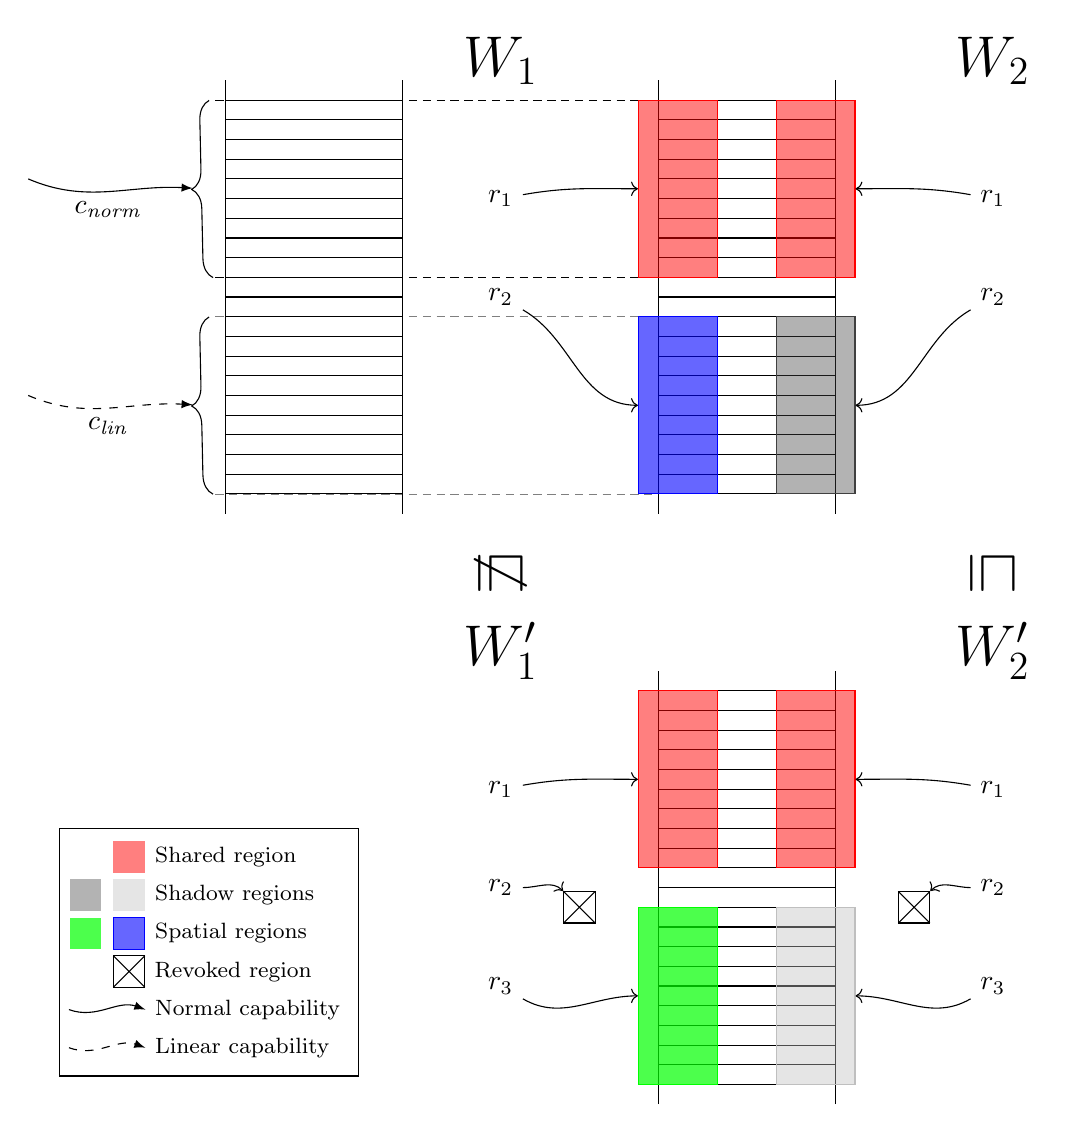
\begin{tikzpicture}[scale=.5, every node={scale=.5}]
    \begin{scope}
  \scope
    \clip (-.1,-.1) rectangle (4.6,11.1);
    \fill[fill=white] (0,0) rectangle (4.5,11);
    \draw (0,0) -- (0,11);
    \draw (4.5,0) -- (4.5,11);
      \foreach \x in {.5,1,...,10}
      {
        \draw[fill=white] (0,\x) rectangle (4.5,\x+.5) node[pos=.5,color=teal] {};
      };
  \endscope
  \draw [decorate,decoration={brace,amplitude=7pt,raise=4pt},yshift=0pt] (-.025,0.5) -- (-.125,5) node (lin) [black,midway,xshift=-0.25cm,align=center] { };
  \draw (-5,3) edge[-latex, bend right, in=180, out=-20, dashed] node[below] {$c_{\var{lin}}$}(lin);
  
  \draw [decorate,decoration={brace,amplitude=7pt,raise=4pt},yshift=0pt] (-.025,6) -- (-.125,10.5) node (norm) [black,midway,xshift=-0.25cm,align=center] { };
  \draw (-5,8.5) edge[-latex, bend right, in=180, out=-20] node[below] {$c_{\var{norm}}$} (norm);

  \draw (-0.25,10.5) edge[very thin, densely dashed, opacity=6] (11,10.5);
  \draw (-0.25,6) edge[very thin, densely dashed, opacity=6] (11,6);
  \draw (-0.25,5) edge[very thin, densely dashed, opacity=0.5] (11,5);
  \draw (-0.25,0.5) edge[very thin, densely dashed, opacity=0.5] (11,0.5);
\end{scope}

  \begin{scope}[shift={(11,0)}]
  \scope
    \clip (-.1,-.1) rectangle (4.6,11.1);
    \fill[fill=white] (0,0) rectangle (4.5,11);
    \draw (0,0) -- (0,11);
    \draw (4.5,0) -- (4.5,11);
      \foreach \x in {.5,1,...,10}
      {
        \draw[fill=white] (0,\x) rectangle (4.5,\x+.5) node[pos=.5,color=teal] {};
      };
  \endscope

  \draw (-4,11.5) node {\huge $W_1$};
  \draw (-4,8) node (w1r1) {$r_1$};
  \draw (-4,5.5) node (w1r2) {$r_2$};

  \draw[red, fill=red, fill opacity=.5] (-.5,10.5) rectangle (1.5,6) node[fitting node] (w1s) { };
  \draw (w1r1) edge[->,in=180, out=10] (w1s.west);

  \draw[blue, fill=blue, fill opacity=.6] (-.5,5) rectangle (1.5,0.5) node[fitting node] (w1l) { };
  \draw (w1r2) edge[->,in=180, out=-30] (w1l.west);


  \draw (8.5,11.5) node {\huge $W_2$};
  \draw (8.5,8) node  (w2r1) {$r_1$};
  \draw (8.5,5.5) node (w2r2) {$r_2$};

  \draw[red, fill=red, fill opacity=.5] (3,10.5) rectangle (5,6) node[fitting node] (w2s) { };
  \draw (w2r1) edge[->,in=0, out=170] (w2s.east);

  \draw[darkgray, fill=darkgray, fill opacity=.4] (3,5) rectangle (5,0.5) node[fitting node] (w2l) { };
  \draw (w2r2) edge[->,in=0, out=210] (w2l.east);

  \end{scope}

  \begin{scope}[shift={(11,-15)}]
  \scope
    \clip (-.1,-.1) rectangle (4.6,11.1);
    \fill[fill=white] (0,0) rectangle (4.5,11);
    \draw (0,0) -- (0,11);
    \draw (4.5,0) -- (4.5,11);
      \foreach \x in {.5,1,...,10}
      {
        \draw[fill=white] (0,\x) rectangle (4.5,\x+.5) node[pos=.5,color=teal] {};
      };
  \endscope

  \draw (-4,11.5) node (w1) {\huge $W_1'$};
  \draw node[above of=w1,rotate=-90] {\huge $\not\sqsubseteq$};
  \draw (-4,8) node (w1r1) {$r_1$};
  \draw (-4,5.5) node (w1r2) {$r_2$};
  \draw (-4,3) node (w1r3) {$r_3$};

  \draw[red, fill=red, fill opacity=.5] (-.5,10.5) rectangle (1.5,6) node[fitting node] (w1s) { };
  \draw (w1r1) edge[->,in=180, out=10] (w1s.west);

  \node[draw,rectangle, black, minimum size=4mm] (w1r) at (-2,5) {  };
  \node[fit=(w1r),black,inner sep=-\pgflinewidth,cross out, draw] (test) { };
  \draw (w1r2) edge[->, out=0] (w1r);

  \draw[green, fill=green, fill opacity=.7] (-.5,5) rectangle (1.5,0.5) node[fitting node] (w1l) { };
  \draw (w1r3) edge[->,in=180, out=-30] (w1l.west);


  \draw (8.5,11.5) node (w2) {\huge $W_2'$};
  \draw node[above of=w2,rotate=-90] {\huge $\sqsubseteq$};
  \draw (8.5,8) node  (w2r1) {$r_1$};
  \draw (8.5,5.5) node (w2r2) {$r_2$};
  \draw (8.5,3) node (w2r3) {$r_3$};

  \draw[red, fill=red, fill opacity=.5] (3,10.5) rectangle (5,6) node[fitting node] (w2s) { };
  \draw (w2r1) edge[->,in=0, out=170] (w2s.east);

  \node[draw,rectangle, black, minimum size=4mm] (w2r) at (6.5,5) {  };
  \node[fit=(w2r),black,inner sep=-\pgflinewidth,cross out, draw] (test) { };
  \draw (w2r2) edge[->, out=180,in=45] (w2r);


  \draw[lightgray, fill=lightgray, fill opacity=.4] (3,5) rectangle (5,0.5) node[fitting node] (w2l) { };
  \draw (w2r3) edge[->,in=0, out=210] (w2l.east);

  \end{scope}

   \matrix [draw,above right, column sep=1.5mm,xshift=.4cm,yshift=.4cm] at (current bounding box.south west) {
    &\node[red, fill=red, fill opacity=.5,minimum size=0.4cm,label=right:{\footnotesize Shared region}] {}; \\
     \node[darkgray, fill=darkgray, fill opacity=.4,minimum size=0.4cm] {};
    &\node[lightgray, fill=lightgray, fill opacity=.4,minimum size=0.4cm,label=right:{\footnotesize Shadow regions}] {}; \\
     \node[green, fill=green, fill opacity=.7,minimum size=0.4cm] {};
    &\node[blue, fill=blue, fill opacity=.6,minimum size=0.4cm,draw,label=right:{\footnotesize Spatial regions}] {}; \\
    &\node[draw,rectangle, black, minimum size=4mm] (rev) {};
     \node[fit=(rev),black,inner sep=-\pgflinewidth,cross out, draw, label=right:{\footnotesize Revoked region}] {};\\
     \node[minimum size=0.4cm] (ln) {}; & \node[minimum size=0.4cm,label=right:{\footnotesize Normal capability}] (rn) {};\\
     \node[minimum size=0.4cm] (ll) {}; & \node[minimum size=0.4cm,label=right:{\footnotesize Linear capability}] (rl) {};\\
};
\draw (ln.west) edge[-latex,out=-20,in=160] (rn.east);
\draw (ll.west) edge[-latex,out=-20,in=160,dashed] (rl.east);

%   \matrix [draw,below right, column sep=1.5mm, anchor=south west] at (current bounding box.south west) {
%     &\node[red, fill=red, fill opacity=.5,minimum size=0.4cm,label=right:{\footnotesize Shared region}] {}; \\
%     &\node[gray, fill=gray, fill opacity=.4,minimum size=0.4cm,label=right:{\footnotesize Shadow region}] {}; \\
%      \node[green, fill=green, fill opacity=.7,minimum size=0.4cm] {};
%     &\node[blue, fill=blue, fill opacity=.6,minimum size=0.4cm,draw,label=right:{\footnotesize Spatial region}] {}; \\
%     &\node[draw,rectangle, black, minimum size=2mm] (rev) {};
%      \node[fit=(rev),black,inner sep=-\pgflinewidth,cross out, draw, label=right:{\footnotesize Revoked region}] {};\\
% };
\end{tikzpicture}

\caption{Example what happens to worlds when a linear capability $c_{\var{lin}}$ is repurposed.
  The linear capability is originally valid with respect to $W_1$.
  In $W_1'$ there is a new spatial region that the linear capability is valid with respect to (the different coloured regions signify different invariants).
  $W_1'$ still has $r_2$, but now it points to a $\revoked$ region.
  This means that $W_1'$ is not a future world of $W_1$.
  The normal capability $c_{\var{norm}}$ is originally valid with respect to $W_2$ and should stay valid with respect to the new world $W_2'$.
The $W_2'$ is a future world of $W_2$ as the $\spatial$ region in $W_2$ is replaced with a $\revoked$ region which is permitted by the future world relation.}
\label{fig:world-example}
\end{figure}

With the future region relation in place, we can define the future world relation as follows: For worlds $W$ and $W'$,
\[
  W' \future W \text{ iff } \left\{
    \array{l}
    \text{for $i \in \{\mathrm{heap},\mathrm{free\_stk},\mathrm{call\_stk} \}$} \\
    \quad\exists m_i : \RegionName \fun \RegionName, \text{ injective}\ldotp\\
    \qquad \dom(W'.i) \supseteq \dom(m_i(W.i)) \wedge \forall r \in \dom(W.i)\ldotp W'.i(m_i(r)) \future W.i(r)
     \endarray
  \right.
\]
The relation says that each of the three worlds must be an extension of the past world and each of the existing regions must have a future region.
% injective function
Note that the future world relation has a mapping function $m_i$ which allows us to change the naming of regions in future worlds.
The definition is a generalization of the standard definition where $m_i$ would be the identity\footnote{In \citet{skorstengaard_reasoning_2017} the future region relation and the reasoning about the awkward example could have been simplified with this future world relation.}.\dominique{I wonder if the renaming function obviates the need for the ``revoked'' trick.}

\subsubsection{Joining worlds}
\label{subsubsec:joining-worlds}
The world serves multiple purposes as it is both a specification of memory contents as well as a specification of authority.
This is best seen in the operators used to join worlds.
First when we see the world as a memory specification, we have a pretty standard join $\uplus$ that simply requires the worlds to have different region names.\begin{definition}[World disjoint union $\uplus$]
  Given worlds $W_1$, $W_2$, $W$
  \[
    W_1 \uplus W_2 = W
    \text{ iff }
    \begin{array}[t]{l}
      \dom(\pwheap) = \dom(\pwheap[W_1]) \uplus \dom(\pwheap[W_2]) \tand \\
      \dom(\pwfree) = \dom(\pwfree[W_1]) \uplus \dom(\pwfree[W_2]) \tand \\
      \dom(\pwpriv) = \dom(\pwpriv[W_1]) \uplus \dom(\pwpriv[W_2]) \\
    \end{array}
  \]
\end{definition}
The $\uplus$ world join does not guarantee that the result is a sensible world with respect to authority or memory specification.
In \sectionname~\ref{subsubsec:mem-sat}, we define memory satisfaction which also acts as a well-formedness judgement.

When we view the world as a specification of authority, then the world join need to respect the region ownership.
That is, when we join the authority of two worlds, then the ownership of the two worlds should not overlap.
This is expressed by the $\oplus$ operator.
\begin{definition}[$\oplus$, disjoint union of ownership]
  \[
    W_1 \oplus W_2 = W
  \text{ iff }
  \begin{array}[t]{l}
    \dom(\pwheap) = \dom(\pwheap[W_1]) = \dom(\pwheap[W_2]) \tand \\
    \dom(\pwfree) = \dom(\pwfree[W_1]) = \dom(\pwfree[W_2]) \tand \\
    \dom(\pwpriv) = \dom(\pwpriv[W_1]) = \dom(\pwpriv[W_2]) \tand \\
    \forall r \in \dom(\pwheap) \ldotp \pwheap(r) = \pwheap[W_1](r) \oplus \pwheap[W_2](r) \tand \\
    \forall r \in \dom(\pwfree) \ldotp \pwfree(r) = \pwfree[W_1](r) \oplus \pwfree[W_2](r) \tand \\
    \forall r \in \dom(\pwpriv) \ldotp \pi_1(\pwpriv(r)) = \pi_1(\pwpriv[W_1](r)) \oplus \pi_1(\pwpriv[W_2](r))
  \end{array}
  \]
  where $\oplus$ for regions is defined as
\begin{align*}
  (\pure,H,H_\sigma) \oplus (\pure,H,H_\sigma) =  & \; (\pure,H,H_\sigma) \\
  (\spatial,H) \oplus (\spatial,H) =  & \; (\spatial,H) \\
  \revoked \oplus \revoked = & \; \revoked \\
  (\spatialo,H) \oplus (\spatial,H) = & \; (\spatial,H) \oplus (\spatialo,H)\\
                                           =  & \; (\spatialo,H)
\end{align*}
\end{definition}
The $\oplus$ operator, like the $\uplus$ operator, does not guarantee that the resulting world is sensible (e.g., the regions are not overlapping).
Only when we know that a certain memory satisfies the world (as a memory specification, see Section~\ref{subsubsec:mem-sat}), will we be sure that the world's specifications are actually non-contradictory.

The $\uplus$ operator is used in the logical relation for components (\sectionname~\ref{subsec:component-rel}) which specifies (among other things) that the world should specify the presence of the component's data memory.
Linking two components then produces a new component with both components' data memory.
The linked component is valid in a world that has the combined memory presence specifications, not the combined authority.

Note also that this picture is further complicated by our usage of non-authority-carrying $\spatial$ regions.
They are really only in a world $W$ as a shadow copy of a $\spatialo$ region in another world $W'$ that $W$ will be combined with.
The shadow copy is used for specifying when a memory satisfies a world: the memory should contain all memory ranges that anyone has authority over, not just the ones whose authority belongs to the memory itself.
For example, if a register contains a linear pointer to a range of memory, then the register file will be valid in a world where the corresponding region is $\spatialo$, while the memory will be valid in a world with the corresponding region only $\spatial$.
However, for the memory to satisfy the world, the block of memory needs to be there, i.e. the memory should contain blocks of memory satisfying every region that is $\spatialo$, $\pure$, but also just $\spatial$ (because it may be $\spatialo$ in, for example, the register file's world).

\subsubsection{Memory satisfaction}
\label{subsubsec:mem-sat}
% Specification
The world can be seen as a specification of the memory contents.
This means that we need to define what it means for a pair of \trgcm{} and \srccm{} memories to satisfy the specification.
% Call stack
The world also keeps track of the structure of the call stack, the allowed uses of designated seals, and linear capability authority, so these things also influence the definition of memory satisfaction.
% Well-formedness
The world definition on its own allows the invariants imposed by regions to be overlapping.
However, to be able to easily determine what invariants a memory segment must respect, we want the invariants of the regions to impose requirements on disjoint parts of the memory.
The memory satisfaction relation makes sure that this is the case, so in a sense the memory satisfaction also acts as a well-formedness judgement for worlds.

\dominique{At this point, the paper is starting to read like a tech report.
  Are we sure it's a good idea to provide this much technical detail?
  I would propose to not include all definitions, but a representative selection and refer to the TR for full detail.
}

Memory satisfaction is split into four definitions.
At the top-level we have $\memSat{\ms_S,\ms_\stk,\stk,\ms_T}{W}$ which relates the source memory triple, $\ms_S$ (heap), $\ms_\stk$ (free stack), and $\stk$ (stack frames), from \srccm{} to the target memory $\ms_T$ from \trgcm{}.
The top-level definition of memory satisfaction splits the target memory in three parts, one for each of the three kinds of source memory.
It also splits the world in three to distribute the authority of the world.
The three $\ms_T$ partitions are related to $\ms_S$, $\ms_\stk$, and $\stk$ by the relations $\lrhname$, $\lrstk[]$, and $\lrfree[]$, respectively. 
The $\lrhname$ relation relates the \srccm{} heap (non-stack memory) to the corresponding heap memory on \trgcm{}.
The $\lrhname$ relation also ensures that the seal invariants associated with each region have invariants on disjoint sets of seals.
The $\lrstk[]$ relation relates the stack of encapsulated stack frames on \srccm{} to the corresponding memory on \trgcm{}.
The layout of the stack determines the call order, so $\lrstk[]$ also makes sure that the placement in memory of the stack frames have the correct order relative to each other and the base address of the stack.
Finally, $\lrfree[]$ relates the free part of the stack of \srccm{} to the corresponding memory segment on \trgcm{}.
$\lrfree[]$ also makes sure that the base address of the stack is actually part of the free stack.
\begin{definition}[Heap relation]
\label{def:heap-rel}
For a set of seals $\overline{\sigma}$, memory segments $ms$ and $\ms_T$, and worlds $W$ and $W'$, we define the heap relation $\lrhname$ as:
\[
  \npair{(\overline{\sigma},\src{ms},\ms_T)} \in \lrheap(\pwheap)(W') = 
  \left\{
    \begin{array}{l}
      \exists R_\ms : \dom(\activeReg{\pwheap}) \fun \MemSeg \times \MemSeg \wedge \\
      \quad \ms_T = \biguplus_{r \in \dom(\activeReg{\pwheap})} \pi_2(R_\ms(r)) \wedge \\
      \quad \src{\ms} = \biguplus_{r \in \dom(\activeReg{\pwheap})} \pi_1(R_\ms(r)) \wedge \\
      \quad \exists R_W : \dom(\activeReg{\pwheap}) \fun \World\ldotp\\
      \qquad W' = \oplus_{r \in \dom(\activeReg{\pwheap})} R_W(r) \wedge\\
      \qquad \forall r \in \dom(\activeReg{\pwheap}), n' < n \ldotp \\
      \qquad \quad \npair[n']{R_\ms(r)} \in  \pwheap(r).H \; \xi^{-1}(R_W(r)) \wedge\\
      \exists R_\var{seal} : \dom(\activeReg{\pwheap}) \fun \powerset{\Seal} \wedge\\
      \quad \biguplus_{r \in \dom(\activeReg{\pwheap})} R_\var{seal}(r)) \subseteq \overline{\sigma} \wedge\\
      \quad \forall r \in \dom(\erase{\pwheap}{\pure})\ldotp \dom(\pwheap(r).H_\sigma) = R_\var{seal}(r)
    \end{array}
  \right.
\]
\end{definition}
Memory satisfaction, and thus also the heap relation, only considers the non-$\revoked$ regions.
The $\lrhname$-relation uses the function $\activeReg{}$ to erase all the $\revoked$ regions from the world.

To a large extent, the definition of $\lrhname$ is pretty standard.
$\lrhname$ assumes the existence of a partitioning of the \trgcm{} and \srccm{} heap memories that can be turned into memory segment pairs each satisfying the invariant of a region.
The heap satisfaction must also respect the world as an authority specification, so the heap satisfaction partitions the authority of the world using $\oplus$.
Each of the memory segment pairs must be in the region invariant with respect to a specific world partition which makes sure that uniqueness of linearity of capabilities is respected.

The heap sub-world contains all seal invariants.
Similar to memory segments, only one seal invariant should impose restrictions on a seal, which $\lrhname$ makes sure is the case.
\begin{definition}[Free stack relation]
\label{def:free-stack-rel}
\[
  \memSatFStack{\src{\ms_\stk},\ms_T}{W} \text{ iff } 
  \left\{
    \begin{array}{l}
      \gc = (\_,\stkb,\_,\_) \wedge\\
      W_\var{stack} = \pwfree \wedge \\
      \exists R_\ms : \dom(\activeReg{W_\var{stack}}) \fun \MemSeg \times \MemSeg \wedge \\
      \quad \ms_T = \biguplus_{r \in \dom(\activeReg{W_\var{stack}})} \pi_2(R_\ms(r)) \wedge \\
      \quad \src{\ms_\stk} = \biguplus_{r \in \dom(\activeReg{W_\var{stack}})} \pi_1(R_\ms(r)) \wedge \\
      \quad \stkb \in \dom(\ms_T) \wedge \stkb \in \dom(\src{\ms_\stk}) \wedge \\
      \quad \exists R_W : \dom(\activeReg{W_\var{stack}}) \fun \World\ldotp\\
      \qquad W = \bigoplus_{r \in \dom(\activeReg{W_\var{stack}})} R_W(r) \wedge\\
      \qquad \forall r \in \dom(\activeReg{W_\var{stack}}),n' < n \ldotp \\
      \qquad \quad \npair[n']{R_\ms(r)} \in  W_\var{stack}(r).H \; \xi^{-1}(R_W(r))
    \end{array}
  \right.
\]
\end{definition}
The free stack relation $\lrfree[]$ is in most regards like the heap relation, $\lrhname{}$.
The free stack relation, partitions the \srccm{} and \trgcm{} free stack memory, it partitions the authority of the world, and it requires the memory segment pairs to be related under part of the world.
For \stktokens{} to work, it should always work on the same stack.
As discussed in \sectionname~\ref{sec:stktokens-explained}, we make sure that it is always the same stack by requiring the address $\stkb$ to be the ''top'' address of the free stack address space.
As the free stack relation relates the stack of \srccm{} with the memory that represents the stack on \trgcm{}, it makes sure that $\stkb$ is the top address of the free stack address space.
\begin{definition}[Stack relation]
  \label{def:stack-rel}
\[
  \memSatStack{\src{\stk},\ms_T}{W} \text{ iff } 
  \left\{
    \begin{array}{l}
      \exists m, \src{\opc_0},\dots,\src{\opc_m}, \src{\ms_0}, \dots, \src{\ms_m}, W_\var{stack}\ldotp\\
      \quad\gc = (\_,\stkb,\_,\_) \wedge \\
      \quad W_\var{stack} = \pwpriv \wedge \\
      \quad\src{\stk} = \src{(\opc_0,\ms_0), \dots (\opc_m,\ms_m)} \wedge \\
      \quad\forall i \in \{0,\dots,m\} \ldotp (\dom(\src{\ms_i}) \neq \emptyset \wedge\\
      \quad\quad \forall j < i \ldotp \forall a \in \dom(\src{\ms_i}) \ldotp \forall a' \in \dom(\src{\ms_j}) \ldotp \stkb < a < a') \wedge\\
      \quad\exists R_\ms : \dom(\activeReg{W_\var{stack}}) \fun \MemSeg \times \Addr \times \MemSeg \ldotp \\
      \quad\quad \ms_T = \biguplus_{r \in \dom(\activeReg{W_\var{stack}})} \pi_3(R_\ms(r)) \wedge \\
      \quad\quad \src{\ms_0} \uplus \dots \uplus \src{\ms_m} = \biguplus_{r \in \dom(\activeReg{W_\var{stack}})} \pi_1(R_\ms(r)) \wedge \\
      \quad\quad \exists R_W : \dom(\activeReg{W_\var{stack}}) \fun \World \ldotp \\
      \quad\qquad W = \bigoplus_{r \in \dom(\activeReg{W_\var{stack}})} R_W(r) \wedge \\
      \quad\qquad \forall r \in \dom(\activeReg{W_\var{stack}}), n' < n\ldotp \\
      \quad\qquad \quad \npair[n']{(\pi_1(R_\ms(r)),\pi_3(R_\ms(r))} \in W_\var{stack}(r).H \; \xi^{-1}(R_W(r)) \wedge\\
      \quad\qquad \quad \pi_2(R_\ms(r)) = W_\var{stack}(r).\opc \wedge\\
      \quad\qquad \quad \exists i \ldotp \src{\opc_i} = W_\var{stack}(r).\opc \wedge \src{\ms_i} = \pi_1 (R_\ms(r))
    \end{array}
  \right.
\]
\end{definition}
The stack relation $\lrstk[]$ is similar to the heap relation in some ways.
The $\lrstk[]$ relation also partitions the \trgcm{} memory but only the \trgcm{} as the \srccm{} partitions are given as the stack frames.
The stack relation also partitions the authority of the world, so it can relate the stack frames in a way that respect linearity.
The stack on \srccm{} represents the call stack which means that each stack frame corresponds to a call and its local data.
The operational semantics of \trgcm{} does not have a built-in stack, so we emulate it by requiring that a stack like data structure resides in \trgcm{} memory.
That is for a memory segment that represents a stack frame, all the addresses of memory frames lower in the stack should have strictly smaller memory addresses.
Further, the stack frames should be in the part of the memory we agree to be the stack which means that the addresses should be smaller than $\stkb$.
Informally, this just means that the stack should be laid out in memory as a downwards growing stack with no addresses below $\stkb$.

According to \stktokens{} (described in \sectionname~\ref{sec:stktokens-explained}), stack frames must be non-empty, so they are distinguishable from a missing stack frame.
For this reason, $\lrstk[]$ requires every stack frame to be non-empty.
Note that each stack frame corresponds to a trusted call.
Untrusted calls are not protected which means that untrusted stack frames reside in the free stack memory (this does not mean that the untrusted stack frames are necessarily unprotected; it only means that they are not natively protected by \stktokens{}).
This means that the protected stack frames are not necessarily packed tightly in memory, and the memory in between is part of the free stack.
The free stack in between stack frames may be used by untrusted code for their local stack frames (Untrusted stack frames are not protected by \srccm{}, but this does not prevent untrusted code from securing their own stack frames).
\figurename~\ref{fig:mem-sketch} sketches this.

Each stack frame in the \srccm{} stack contains an old program pointer which corresponds to the old program counter recorded in the region of the world associated with the stack frame.
To achieve this, the partition function $R_\ms$ also records an $\opc$ for each region, and this $\opc$ should establish the link between the region and the stack frame.
\begin{figure}
  \centering
  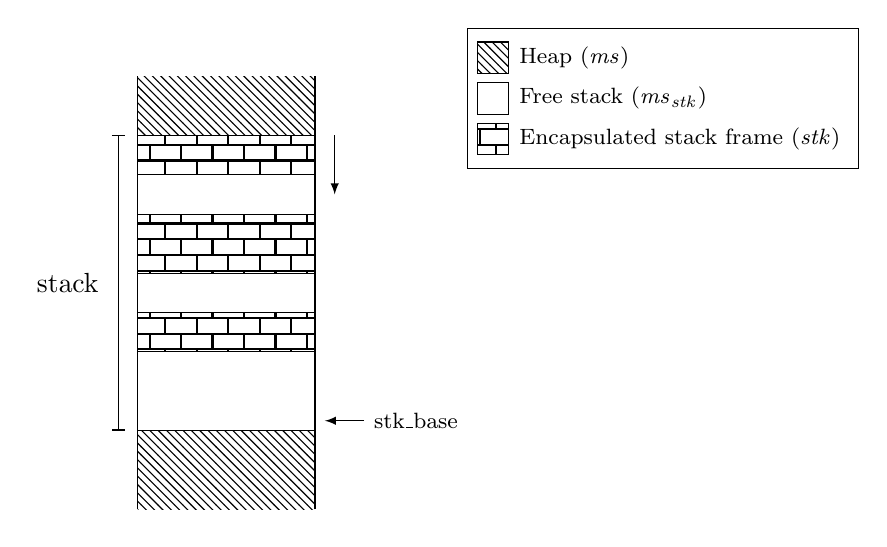
\begin{tikzpicture}[scale=.5, every node={scale=.5}]
 
  \scope
    \clip (-.1,-.1) rectangle (4.6,11.1);
    \fill[fill=white] (0,0) rectangle (4.5,11);
    \draw (0,0) -- (0,11);
    \draw (4.5,0) -- (4.5,11);
  \endscope
  \draw (-1,0) node {};
  \draw (-1,12) node {};

  \draw[pattern=north west lines,draw=none] (0,0) rectangle (4.5,2);
  \draw[pattern=north west lines,draw=none] (0,9.5) rectangle (4.5,11);

  \draw[pattern=none] (0,2) rectangle (4.5,4);
  \draw[pattern=bricks] (0,4) rectangle (4.5,5);
  \draw[pattern=none] (0,5) rectangle (4.5,6);
  \draw[pattern=bricks] (0,6) rectangle (4.5,7.5);
  \draw[pattern=none] (0,7.5) rectangle (4.5,8.5);
  \draw[pattern=bricks] (0,8.5) rectangle (4.5,9.5);

  \draw (5.75,2.25) node[anchor=west] {\footnotesize $\stkb$};
  \draw (5.75,2.25) edge[-latex] (4.75,2.25);
  \draw (5,9.5) edge[-latex] (5,8);
%  \draw [decorate,decoration={brace,amplitude=7pt,mirror,raise=4pt},yshift=0pt] (-0.25,9.5) -- (-0.25,2) node [black,midway,xshift=-1cm,yshift=0.05cm,rotate=45] {stack};
  \draw [-|] (-0.5,9.5) edge (-0.5,2);
  \draw (-0.75,5.75) node[anchor=east] [black] {stack};
  \matrix [draw,below right] at (current bounding box.north east) {
    \node[pattern=north west lines,minimum size=0.4cm,draw,label=right:{\footnotesize Heap ($\ms$)}] {}; \\
    \node[minimum size=0.4cm,draw,label=right:{\footnotesize Free stack ($\ms_\stk$)}] {}; \\
    \node[pattern=bricks,minimum size=0.4cm,draw,label=right:{\footnotesize Encapsulated stack frame ($\stk$)}] {}; \\
};

  \end{tikzpicture}
  \caption{A sketch of how heap, encapsulated stack and free stack are laid out in memory.
    The encapsulated stack frames and the free stack constitutes the stack.
    The encapsulated stack frames may have free stack in between them where stack frames of non-trusted code may reside.
    The stack grows downwards in memory with $\stkb$ as the top address (and the base address of the free stack capability).}
  \label{fig:mem-sketch}
\end{figure}

In order to tie Definitions~\ref{def:heap-rel},~\ref{def:free-stack-rel},~and~\ref{def:stack-rel} together, we define memory satisfaction.
Memory satisfaction defines when a \srccm{} memory, consisting of a heap, a stack, and a free stack, relates to a \trgcm{} memory under a world.
\begin{definition}[Memory satisfaction]
  For memory segments $\ms_S$, $\ms_\stk$, and $\ms_T$, stack $\stk$, and world $W$ we define memory satisfaction as
\[
  \memSat{\src{\ms_S},\src{\ms_\stk},\src{\stk},\ms_T}{W} \text{ iff } 
  \left\{
    \begin{array}{l}
      \exists m,  \src{\opc_0}, \dots \src{\opc_m}, \src{\ms_0}, \dots, \src{\ms_m}, W_{\var{stack}}, W_{\var{free\_stack}}, W_{\var{heap}} \ldotp\\
      \quad \src{\stk} = \src{(\opc_0,\ms_0):: \dots :: (\opc_m,\ms_m)} \wedge \\
      \quad \src{\ms_S} \# \src{\ms_\stk} \# \src{\ms_0} \# \dots \# \src{\ms_m} \wedge\\
      \quad W = W_{\var{stack}} \oplus W_{\var{free\_stack}} \oplus W_{\var{heap}} \wedge\\
      \quad\exists \ms_\var{T,stack}, \ms_\var{T,free\_stack}, \ms_\var{T,heap}, \ms_{T,f}, \src{\ms_{S,f}}, \src{\ms_S'},\overline{\sigma}\ldotp \\
      \qquad \src{\ms_S} = \src{\ms_{f,S}} \uplus \src{\ms_S'} \wedge \\
      \qquad \ms_T = \ms_\var{T,stack} \uplus \ms_\var{T,free\_stack} \uplus \ms_\var{T,heap} \uplus \ms_{T,f} \wedge \\
      \qquad \dom(\ms_{\var{T,stack}} \uplus \ms_\var{T,free\_stack}) = [\baddr_\stk,\eaddr_\stk] \wedge \\
      \qquad \baddr_\stk -1,\eaddr_\stk + 1 \in \dom(\ms_{T,f}) \wedge \\
      \qquad \memSatStack{\src{\stk},\ms_\var{T,stack}}{W_{\var{stack}}} \wedge \\
      \qquad \memSatFStack{\src{\ms_\stk},\ms_\var{T,free\_stack}}{W_{\var{free\_stack}}} \wedge \\
      \qquad \npair{(\overline{\sigma},\src{\ms_S'},\ms_\var{T,heap})} \in \lrheap(\pwheap)(W_{\var{heap}})
    \end{array}
  \right.
\]
\end{definition}
Memory satisfaction partitions the \trgcm{} memory in a heap, stack frames, a free stack and a frame.
The \srccm{} heap is split in two: the active heap and a frame.
Our configurations describe the complete machine state, but we may only be interested in the invariants on part of it.
The frame allows us to ignore the part of the memory that won't affect the computation.
Just like the previous memory relations, the world is split in three to make sure that linearity is respected.
Each part of the \srccm{} memory is related to the appropriate part of the memory from \trgcm{} by the relevant relation under a partition of the world.

\stktokens{} requires the stack to not be adjacent to heap or code memory.
This is enforced in the memory satisfaction by requiring that the addresses adjacent to the memory are in the frame.

% TODO take a look at notation and naming in this section. What do we want to call things
% TODO look over the original POPL paper to make sure to reuse all the text that makes sense to reuse.
\end{jversion}


\subsection{Constructing Worlds: Solving the Recursive Domain Equation}
\label{sec:rec-dom-eq}
In the previous sections, we sketched what our worlds should be.
However, the worlds we want constitute a self-referential domain equation for which no solution exists in set and domain theory.
% Move to a different domain
Therefore, we need to move to a different domain with enough structure for a solution to exist for recursive equations.
Solutions to recursive domain equations can be found using standard techniques~\citep{scott_1976,america_1989,Birkedal:2011:SKM:1926385.1926401}.
Essentially, we move to a setting where instead of sets we have c.o.f.e.'s (complete ordered families of equivalences), instead of functions we have non-expansive functions, and instead of relations we have downwards-closed relations.
A c.o.f.e.\ can be thought of as a set with added structure, specifically a step-indexed notion of equality and a limit to every Cauchy sequence (i.e.\ they are complete in a similar sense as to how the real numbers are complete but the rationals are not).

Explaining the construction of the world in detail would require a recap of the basic theory of c.o.f.e.'s.
For conciseness, we choose to not include this here, but instead refer to the PhD thesis of Skorstengaard \cite[\S 3.5]{skorstengaard_thesis_2019}, which includes a detailed explanation.
We only include the main result, which is the following theorem, asserting the existence of a World c.o.f.e.\ satisfying the recursive equation we encountered before.

% In this section, we explain our solution of the world equation.
% To make this paper self-contained, we include a recap of relevant concepts and theorems from the literature on c.o.f.e.'s.
% This section does not provide further intuition about the worlds and can be safely skipped.

% Recursive domain equations are so common and the solution so standard that frameworks implement them to lift the technical burden of constructing the world by hand.
% The technique we use to solve our recursive domain equation is essentially the same as what is used internally in the program logic framework Iris~\citep{iris,iris2,iris3} to construct worlds.
% We believe the worlds presented here could be developed in Iris.
% Had we done the development in Iris Coq, then we would have had the world tool support of Iris and the rigorousness of Coq which, in hindsight, would have been very beneficial.

% % Cofe's
% In this section, we explain how the world is constructed in detail (readers willing to trust us can safely skip to Section~\ref{subsubsec:joining-worlds}).
% To explain this, we present complete ordered family of equivalences \citep{di_gianantonio_2002}.
% We loosely follow the presentation in \citet{birkedal_taste_2014} and introduce the necessary definitions needed for our particular world.
% \begin{definition}[Ordered family of equivalences (o.f.e.)]
% An \emph{ordered family of equivalences} is a pair $\cofe{X}$ where $X$ is a set and $\nequal$ is an equivalence relation for each $n$.
% The pair must satisfy the following properties:
% \begin{enumerate}
% \item $\nequal[0]$ is the total relation.
% \item For all $n \in \nats$, $\nequal[n] \supseteq \nequal[n+1]$.
% \item For all $x,y \in X$,  if for all $n \in \nats$ $x \nequal y$, then $x = y$.
% \end{enumerate}
% \end{definition}
% \noindent An o.f.e.\ can be thought of as a set with extra structure.
% Intuitively, the index on the family of equivalences is a measure of precision.
% The larger the index is, the more refined the equivalences are which means that they can distinguish more elements from one another.
% On the other hand as the index decreases, the equivalences become increasingly imprecise and unable to distinguish certain elements.
% At index 0, all precision is lost and the equivalence cannot distinguish anything.
% \dominique{Introduce phrases like ``up to n steps'' etc.}
% \begin{definition}[Complete ordered family of equivalences (c.o.f.e.)]
%   \label{def:cauchy-sequence}
%   A \emph{complete ordered family of equivalences} is an ordered family of equivalences
%   $\cofe{X}$ such that every Cauchy sequence in $X$ has a limit
%   in $X$.

%   Let $\cofe{X}$ be an o.f.e. and $\seq{x}$ be a sequence of
%   elements in $X$. Then $\seq{x}$ is a \emph{Cauchy sequence} if
%   \begin{align*}
%     \forall k \in \nats, \exists j \in \nats, \forall n \geq j, x_j \nequal[k] x_n
%   \end{align*}
%   or in words, the elements of the chain get arbitrarily close.

%   An element $x \in X$ is the \emph{limit} of the sequence $\seq{x}$ if
%   \begin{align*}
%     \forall k \in \nats, \exists j \in \nats, \forall n \geq j, x \nequal[k] x_n.
%   \end{align*}
% \end{definition}
% In order to move from one c.o.f.e.\ to another, we define functions, just like we would when working with sets.
% Unlike functions between sets, functions between c.o.f.e.'s must preserve the c.o.f.e.\ structure which informally means that the measure of precision must be retained.
% This specifically means that functions between c.o.f.e.'s must be \emph{non-expansive} which basically means that they preserve $n$-equalities.
% Functions may not only retain equivalences but make it more precise.
% Such a function is said to be \emph{contractive}.
% \begin{definition}
%   \label{def:nonexpansive-contractive-ofe}
%   Let $\left(X,\left(\nequal[n]_X\right)_{n=0}^{\infty} \right)$ and $\left(Y,\left(\nequal[n]_Y\right)_{n=0}^{\infty} \right)$ be two ordered families of equivalences and $f$ a function from the set $X$ to the set $Y$.
%   The function $f$ is
%   \begin{description}
%   \item[non-expansive] when for all $x, x' \in X$, and all $n \in \nats$,
% \[
%   x \nequal_X x' \implies f(x) \nequal_Y f(x')
% \]
%   \item[contractive] when for any $x, x' \in X$, and any $n \in \nats$,
% \[
%   x \nequal_X x' \implies f(x) \nequal[n+1]_Y f(x') 
%   \qedhere
% \]
%   \end{description}
% \end{definition}
% \noindent The step-indexing provided by c.o.f.e.'s give enough structure to solve the recursive domain equation.
% There are a number of standard c.o.f.e.\ constructions for countably sets, products, sums, and functions.
% A set can be lifted to c.o.f.e.\ by having the normal equality for all positive indices and the total relation for $\nequal[0]$.
% The other standard constructions are defined naturally and compose new c.o.f.e.'s from existing c.o.f.e.'s.

% In some sense, the standard c.o.f.e.\ constructions maintain the precision of the underlying c.o.f.e.'s.
% This, however, does not utilise the c.o.f.e.\ structure in a way that allows us to construct a solution for a recursive domain equation.
% Intuitively, the step of the c.o.f.e.\ needs to go down before the recursive occurrence.
% To this end, we have the \emph{later} ($\blater$) c.o.f.e.:
% \begin{lemma}[$\blater$ c.o.f.e.]
%   \label{def:later-cofe}
%   Given a c.o.f.e $\left(X, \left(\nequal_X\right)_{n=0}^{\infty} \right)$ define the later c.o.f.e.\ as
%   \[
%     \blater\left(X, \left(\nequal_X\right)_{n=0}^{\infty} \right) = \left(X, \left(\nequal[n]_{\blater}\right)_{n=0}^{\infty} \right)
%   \]
%   where
%   \[
%     x \nequal[n]_{\blater} x' \text{ iff } \left\{
%       \begin{array}{l}
%         n = 0 \text{ or }\\
%         x \nequal[n-1]_X x'
%       \end{array}
%     \right. \qedhere
%   \]
% \end{lemma}
% The later c.o.f.e.\ should be placed before the self-reference to make the index decrease. 
% Intuitively, this gives something to recurse on in order to find a solution for the domain equation.
% If we limit ourselves to a handful of standard constructions (product, sum, arrow, later, and partial functions from the natural numbers) to construct self-referential equations and make sure to guard every occurrence of the self reference with a later, then the equation has a solution.

% Unfortunately, the standard c.o.f.e.\ constructions do not suffice for the worlds we want to define.
% The worlds we sketched have additional structure in terms of a future world relation.
% The future world relation is captured by adding a preorder to c.o.f.e.'s:
% \begin{definition}[Preordered c.o.f.e.]
%   A preordered c.o.f.e.\ is a c.o.f.e.\ equipped with a preorder on $X$, $\left(X, \left(\nequal\right)_{n=0}^{\infty}, \future \right)$. 
%   \begin{itemize}
%   \item The ordering preserves limits. That is, for Cauchy sequences $\{a_n\}_n$ and $\{b_n\}_n$ in $X$ if $\{a_n\}_n \future\{b_n\}_n$, then $\lim \{a_n\}_n \future \lim \{b_n\}_n$.
%   \end{itemize}
% \end{definition}
% The preorder must respect the existing structure of the c.o.f.e.'s which means that it must preserve limits.
% There are also natural constructions for preordered c.o.f.e.'s that rely on the underlying preorder.
% We will need the standard construction for later, product, and sum (defined in \appendixname~\ref{app:cofe}).

% Sometimes we will refer to c.o.f.e.'s and preordered c.o.f.e.'s simply by their underlying set.

% In the following, we will define a number of preordered c.o.f.e.'s that can be combined to get our world equation.
% First, we define the c.o.f.e.\ for the memory invariants (we do not need a preorder here).
% As a reminder, we sketched the memory invariants to as follows
% \[
%   \World \monfun \Rel{\MemSeg \times \MemSeg}
% \]
% To construct this, we need to define a c.o.f.e.\ for the relation and a c.o.f.e.\ for the monotone and non-expansive functions.
% We do not need a construction for the world as it will be given as the solution to the recursive equation.
% Generally, we can lift a set of relations to a c.o.f.e.\ by adding a downwards closed index to it.
% This means that if a pair is in the relation for a specific index, then it is also in the relation for all smaller indices.
% %% URel
% \begin{definition}[Uniform relation]
%   \label{def:uniform-rel-cofe}
%   Given a set $R = X \times Y$, we define $\URel{R} \subseteq \powerset{\nats \times R}$ as
%   \[
%     \URel{R} = \{ A \in \powerset{\nats \times R} \mid \forall n \in \nats \ldotp \forall r \in R \ldotp \npair{r} \in A \implies \forall m \leq n \ldotp \npair[m]{r} \in A\}
%   \]
%   The uniform relation c.o.f.e.\ $\cofe{\URel{R}}$ has $\URel{R}$ as the underlying set and the following family of equivalences:
%   \[
%     A \nequal B \text{ iff } \erasen{A}{n} = \erasen{B}{n}
%   \]
%   where erasure is defined as
%   \[
%     \erasen{A}{n} \defeq \{(k,a) \in A \mid k < n\}
%   \]
%   to get a preordered c.o.f.e.\ we use subset as the preorder.
% \end{definition}
% The uniform relation construction uses the canonical family of equivalences which basically ignores everything from the step up and requires the rest to be equal.
% This means that everything is equal at step $0$ as everything is left out.

% Next, we define a c.o.f.e.\ of monotone, non-expansive functions
% \begin{definition}[The c.o.f.e. of monotone and non-expansive functions]
% \label{def:monnefun-cofe}
%   Given a preordered c.o.f.e. $\left(W,\left(\nequal[n]_W\right)_{n=0}^{\infty},\future_W\right)$ and a preordered c.o.f.e.\ $\left(U,\left(\nequal[n]_U\right)_{n=0}^{\infty},\future_U\right)$ , define the c.o.f.e.\ $\left(W \monnefun U,\left(\nequal[n]\right)_{n=0}^{\infty}\right)$ where 
%   \[
%     h \nequal h' \text{ iff } \forall w \in \dom(h) \ldotp h(w) \nequal_U h'(w)
%   \]
% \end{definition}
% In order to construct the memory invariant, we use Definition~\ref{def:monnefun-cofe} with the world solution as the $W$ c.o.f.e.\  and a uniform relation over pairs of memory segments (Definition~\ref{def:uniform-rel-cofe}) as the $U$ c.o.f.e.

% Next, we construct the seal invariant.
% As a reminder, we sketched the seal invariant as
% \[
%   \Seal \parfun \World \monnefun \URel{\SealableCaps\times\SealableCaps}
% \]
% In order to define the c.o.f.e. for this, we can use Definitions~\ref{def:uniform-rel-cofe} and~\ref{def:monnefun-cofe}.
% This leaves us with the task of lifting the set of seals to a c.o.f.e.\ and defining the c.o.f.e.\ partial functions.
% Generally, all countable sets can be lifted to a c.o.f.e.\ with a family of equivalences that has full precision for all indices except index 0.
% \begin{definition}[Sets to c.o.f.e.]
%   \label{def:lift-set-cofe}
%   A countable set $S$ can be lifted to a c.o.f.e. $\cofe{S}$ where
%   \begin{itemize}
%   \item $\nequal[0]$ is the total relation
%   \item for $n > 0$ the relation $\nequal$ is the normal equality on the set
%   \end{itemize}
% \end{definition}
% This definition can be used to lift the set of all seals $\Seal$ to a c.o.f.e.

% The c.o.f.e.\ of partial, non-expansive functions is defined similarly to the c.o.f.e.\ of monotone non-expansive functions.
% \begin{definition}[The c.o.f.e. of partial, non-expansive functions]
% \label{def:parfun-cofe}
%   Given a c.o.f.e. $\left(S,\left(\nequal[n]_S\right)_{n=0}^{\infty}\right)$ and a c.o.f.e.\ $\left(H,\left(\nequal[n]_H\right)_{n=0}^{\infty}\right)$ , define the c.o.f.e.\ $\left(S \parfun H,\left(\nequal[n]\right)_{n=0}^{\infty} \right)$ where 
%   \[
%     h \nequal h' \text{ iff } \dom(h) = \dom(h') \wedge \forall w \in \dom(h) \ldotp h(w) \nequal_H h'(w)
%   \]
% \end{definition}
% The seal invariant is defined using Definition~\ref{def:lift-set-cofe} to lift $\SealableCaps$ to a c.of.e.\, defining a c.o.f.e.\ similar to the one for memory invariants, and finally combining the two with Definition~\ref{def:parfun-cofe}.

% Next, we want to define the regions of the world.
% As mentioned, our regions have the added structure of the future region relation, so we need to define them as a preordered c.o.f.e.
% The future region was presented in Section~\ref{subsubsec:ft-and-revocation}.
% On shared regions, the relation is equality which makes it straight forward to define:
% \begin{definition}[Shared region preordered c.o.f.e.\ ]
%   \label{def:pure-reg-p-cofe}
%   Given two c.o.f.e.'s $\left(\var{MemInv},\left(\nequal[n]_\var{MI}\right)_{n=0}^{\infty}\right)$ and $\left(\var{SealInv},\left(\nequal[n]_{\var{SI}}\right)_{n=0}^{\infty}\right)$, define the preordered c.o.f.e.\ of shared regions as
%   \[
%   \left(\{\pure\}\times \var{MemInv} \times \var{SealInv},\left(\nequal[n]\right)_{n=0}^{\infty},=\right)
%   \]
%   where the family of equivalences distributes to the underlying c.o.f.e.'s, i.e. given shared regions $(\pure,H,H_\sigma), (\pure,H',H_\sigma') \in \{\pure\}\times \var{MemInv} \times \var{SealInv}$,
%   \[
%   (\pure,H,H_\sigma) \nequal (\pure,H',H_\sigma') \text{ iff } H \nequal_\var{MI} H' \wedge H_\sigma \nequal_{SI} H_\sigma'
%   \]
% \end{definition}
% Definition~\ref{def:pure-reg-p-cofe} gives us the shared region for preorder c.o.f.e.\ when we use it with the memory invariant c.o.f.e.\ as $\var{MemInv}$ and the seal invariant c.o.f.e.\ as $\var{SealInv}$.

% Next, we define the preordered c.o.f.e.\ for spatial regions.
% The future region relation on spatial regions is non-trivial, so the definition of the preordered c.o.f.e.\ is slightly more involved.
% \begin{definition}[Spatial region preordered c.o.f.e.\ ]
%   \label{def:spatial-reg-p-cofe}
%   Given two c.o.f.e.'s $\left(\var{MemInv},\left(\nequal[n]_\var{MI}\right)_{n=0}^{\infty}\right)$ and $\left(\var{MemInv'},\left(\nequal[n]_\var{MI'}\right)_{n=0}^{\infty}\right)$, let
%   \[
%     \Regions = \{\spatial\}\times \var{MemInv} \cup \{\spatialo\} \times \var{MemInv'} \cup \{\revoked\}
%   \]
%   define the preordered c.o.f.e.\ of shared regions as
%   \[
%   \left(\Regions,\left(\nequal[n]\right)_{n=0}^{\infty},\future\right)
%   \]
%   where the preorder $\future$ is defined as
%   \begin{mathpar}
%   \inferrule{ r \in \Regions }{ r \future r }
%   \and
%   \inferrule{ }{ \revoked \future (\spatial,\_)}
%   \and
%   \inferrule{ }{ (\spatialo,H) \future (\spatial,H)}
%   \end{mathpar}
%   and $\left(\nequal[n]\right)_{n=0}^{\infty}$ is the total relation for $n=0$ and otherwise the region tags must be the same and the memory invariants $n$-equal, i.e.\ 
%   for $r ,r' \in \Regions$ we have $r \nequal r'$ when one of the following holds
%   \begin{itemize}
%   \item $n=0$
%   \item $n > 0$ and one of the following is true
%     \begin{itemize}
%     \item $r = r' = \revoked$
%     \item $r = (\spatial,H)$, $r' = (\spatial,H')$, and $H \nequal_\var{MI} H'$
%     \item $r = (\spatialo,H)$, $r' = (\spatialo,H')$, and $H \nequal_\var{MI'} H'$
%     \end{itemize}
%   \end{itemize}
% \end{definition}
% Definitions~\ref{def:pure-reg-p-cofe} and~\ref{def:spatial-reg-p-cofe} define the preordered c.o.f.e.'s necessary for the regions in our worlds.

% Next, we need to define the three sub-worlds for heap, encapsulated stack frames, and free stack.
% The definitions of the sub-worlds are very similar, so we can capture the essence of all three sub worlds in one definition.
% \begin{definition}[Sub-world preordered c.o.f.e.]
%   \label{def:sub-world-p-cofe}
%   Given preordered c.o.f.e. $\left(\var{Reg},\left(\nequal[n]_\var{Reg}\right)_{n=0}^{\infty},\future_\var{Reg}\right)$ define the sub-world preordered c.o.f.e.\ as
%   \[
%     \left(\nats \parfun \var{Reg},\left(\nequal[n]\right)_{n=0}^{\infty},\future \right)
%   \]
%   where the family of equivalences is defined by given $W,W' \in \nats \parfun \var{Reg}$,
%   \[
%     W \nequal W' \text{ iff } \dom(W) = \dom(W') \wedge \forall r \in \dom(W)\ldotp W(r) \nequal W'(r)
%   \]
%   and the future world relation is defined by given $W,W' \in \nats \parfun \var{Reg}$,
%   \[
%   W' \future W \text{ iff } \left\{
%     \array{l}
%     \exists m : \RegionName \fun \RegionName, \text{ injective}\ldotp\\
%     \quad \dom(W') \supseteq \dom(m(W)) \wedge \forall r \in \dom(W)\ldotp W'.i(m(r)) \future W(r)
%      \endarray
%   \right.
% \]
% \end{definition}
% The free stack sub-world preordered c.o.f.e.\ is constructed from the spatial region preordered c.o.f.e.\ (Definition~\ref{def:spatial-reg-p-cofe}) and the general sub-world construction in Definition~\ref{def:sub-world-p-cofe}.
% The result is the sub-world for the free stack
% \[
%   \Worldfs = \nats \parfun \Regions
% \]

% Next, we define the call stack sub-world.
% To this end, we use Definition~\ref{def:spatial-reg-p-cofe} to get the spatial region which we need to combine this with an address.
% We lift the set of addresses to a preordered c.o.f.e.\ $A$ (Definition~\ref{def:lift-set-cofe} with equality as the preorder) and combine the preordered c.o.f.e.'s $\Addr$ and $\Regions$ with the standard product construction.
% All in all, we get the a preordered c.o.f.e.\
% \[
%   \Regions \times \Addr
% \]
% which we use with Definition~\ref{def:sub-world-p-cofe} to get the preordered c.o.f.e.\ for the stack sub-world:
% \[
%   \Worlds = \nats \parfun \Regions \times \Addr
% \]

% Finally, we define the sub-world for the heap.
% To this end, we combine the shared region preordered c.o.f.e.\ (Definition~\ref{def:pure-reg-p-cofe}) with the spatial region preordered c.o.f.e.\ (Definition~\ref{def:spatial-reg-p-cofe}) using the standard union preordered c.o.f.e.\ construction.
% The result is a preordered c.o.f.e.\
% \[
%   \Regions \cup \Regionh
% \]
% which we use in the sub-world construction (Definition~\ref{def:sub-world-p-cofe}) to obtain the preordered c.o.f.e.\
% \[
%   \Worldh = \nats \parfun (\Regions \cup \Regionh)
% \]

% With the three sub-worlds defined, we combine them with the standard product construction for preordered c.o.f.e.'s to get our worlds.
% \[
%   \Worldh \times \Worlds \times \Worldfs
% \]
% This is the world, we would like to work with, but we still don't have a solution for the recursive domain equation.
% In fact, when we defined the regions, we just left world-index in the memory and seal invariants as an unspecified variable, which means that the above world has them as a variable.
% In order to find a solution, we still need to guard the recursive occurrence.
% To this end, we simply use the construction for later preordered c.o.f.e.'s in Definition~\ref{def:later-p-cofe} with the above to get.
% \[
%   \blater (\Worldh \times \Worlds \times \Worldfs)
% \]
% Now the recursive occurrence is guarded which means that there is a solution to the recursive domain equation.
\begin{theorem}
  \label{thm:rec-dom-eq-sol}
  There exists a complete ordered family of equivalences (c.o.f.e.) $\Wor$ and preorder $\future$ such that $(\Wor,\future)$ is a preordered c.o.f.e., and there exists an isomorphism $\xi$ such that
  \[
    \xi : \Wor \cong \blater (\Worldh \times \Worlds \times \Worldfs)
  \]
  and for $\hat{W},\hat{W}' \in \Wor$
  \[
    \hat{W}' \future \hat{W} \text{ iff } \xi(\hat{W}') \future \xi(\hat{W})
  \]
  for $\Worlds$, $\Worldh$, and $\Worldfs$ defined as follows
\[
  \Worldh = \RegionName \parfun (\Regions \cup \Regionh)
\]
and
\[
  \Worlds = \RegionName \parfun (\Regions \times \Addr)
\]
and
\[
  \Worldfs = \RegionName \parfun \Regions
\]
where $\RegionName = \nats$. $\Regions$ and $\Regionh$ defined as follows
\begin{multline*}
  \Regionh = 
  \{\pure \} \times (\Wor \monnefun \URel{\MemSeg\times\MemSeg}) \times \\
  (\Seal \parfun \Wor \monnefun \URel{\SealableCaps\times\SealableCaps})
\end{multline*}
and
\[
  \Regions = \left\{
  \begin{array}{l}
    \{\spatial, \spatialo\} \times (\Wor \monnefun \URel{\MemSeg\times\MemSeg}) \cup\\
    \{\revoked\}
  \end{array} \right.
\]
\end{theorem}
Theorem~\ref{thm:rec-dom-eq-sol} uses the method of~\citet{Birkedal:2011:SKM:1926385.1926401,birkedal_taste_2014} to construct the solution $\Wor$ to the recursive equation.
Note, that $\Wor$ is not equal to $\blater (\Worldh \times \Worlds \times \Worldfs)$; it is isomorphic.
This means that whenever we encounter $\Wor$, we have to apply $\xi$ and go under a later before we can actually use the world.
This makes it rather inconvenient to have $\Wor$ as the world, so instead we define the worlds as 
\[
  \World = \Worldh \times \Worlds \times \Worldfs
\]

%% Lau: not sure whether the following remarks should be included:
% Note that the later placement could have been different as it just needs to guard the recursive occurrence at some level.
% It could, for instance, have been directly on the recursive occurrence.
% By moving the later, we would also move the place we have to go under the later in our later definitions affecting how it is working with them.

% In worlds that has a simple future world relation and no future region relation, it may be an advantage to define the regions in terms of a self-referential equation, solve that, and define the worlds with the solution.
% The advantage of this approach is that it can be done entirely in c.o.f.e.'s.





\subsection{The Logical Relation}
\begin{jversion}
\label{subsec:logical-relation}
Using these Kripke worlds as assumptions, we can then define when different \srccm{} and \trgcm{} entities are related: values, jump targets, memories, execution configurations, components etc.
The most important relations are summarised in the following table, where we mention the general form of the relations, what type of things they relate and extra conditions that some of them imply:\\
% latex hack stolen from https://tex.stackexchange.com/questions/78788/align-equations-over-multiple-tabular-rows
% Lau: I find it difficult to easily see what constitutes a row in this table.
% I have updated it to a table I find easier to read.
\newcolumntype{R}{>{$}r<{$}}
\newcolumntype{L}{>{$}l<{$}}
\newcolumntype{M}{R@{${}\in{}$}L}
\begin{tabular}{|M|c|p{4.8cm}|}
  \hline
  \multicolumn{2}{|c|}{General form} & Relates ... & and ...\\
  \hline
  \npair{(\src{w_S},w_T)} & \lrv(W) & values (machine words) & safe to pass to adversarial code\\
  \npair{(\src{w_S},w_T)} & \lrvtrusted(W) & values (machine words) & \\
  \npair{(\src{\reg_S},\reg_T)}  &  \lrr(W) & register files & safe to pass to adversarial code\\
  \npair{\src{\Phi_S},\Phi_T}  &  \lro & execution configurations & \\
  \npair{(\src{w_S},w_T)}  &  \lre(W) & $\tjmp{}$ targets &\\
  \left(\arraycolsep=1pt\array{l}(\src{w_{S,1}},\src{w_{S,2}}),\\(w_{T,1},w_{T,2})\endarray\right)  &  \lrexj(W) & $\txjmp{}{}$ targets &\\
  \multicolumn{2}{|c|}{$\memSat{\src{\ms_S},\src{\stk},\src{\ms_\stk},\ms_T}{W}$} & memory & satisfy the assumptions in $W$\\
  \hline
\end{tabular}\\
In Section~\ref{subsubsec:mem-sat}, we already defined memory satisfaction, the relation for memories.
In the following, we define each of the remaining relations and give some intuition about the definitions.
The logical relation we define ends up as a cyclic definition.
The circularity is resolved by another use of step-indexing in the definitions, but the circularity also poses a chicken and egg problem with respect to the order in which the definitions of the relations should be presented.
There is no canonical way of presenting the logical relation as we are bound to make forward references.
For this reason, we suggest making a cursory first read through to get an overview followed by a more thorough read.
% TODO something about relation naming?

\subsubsection{Observation relation}
The observation relation defines what machine configurations have related and permissible observable effects.
Generally speaking, an observation relation captures the property we want to prove.
Ultimately, we want to prove a full-abstraction theorem which is defined in terms of contextual equivalence for components that in turn is defined as co-termination in any context.
This means that the observation relation should capture co-termination.

So far, we have talked about the logical relation as though we define one.
However, we actually define two logical approximations that only differ in the observation relation.
We define a \srccm{} configuration to logically approximate a \trgcm{} configuration when the halting termination of the \srccm{} configuration implies the halting termination of the \trgcm{} configuration.
This also means that \srccm{} configurations that terminates by failing termination are related to any \trgcm{} configuration.
Intuitively, this is because the $\failed$ configuration signals that there was an attempt to break the guarantees of the capability machine.
For instance, a piece of code could have attempted to read from a part of memory it does not have access to, or a callee could have attempted to return out of order.
In both cases, we haven't defined a way to recover from such attempts to break the guarantees, so we are content with failure.
\begin{multline*}
  \lro[\preceq,(\ta,\stkb,\_,\_)] \defeq \\\left\{ \npair{\left(\array{l}\src{(\ms_S,\reg_S,\stk_S,\ms_{\stk,S})},\\(\ms_T,\reg_T)\endarray\right)} \middle|
    \begin{array}{l}
      \forall i \leq n \ldotp \\
      \quad \src{(\ms_S,\reg_S,\stk_S,\ms_{\stk,S})} \sterm[i]{\ta,\stkb} \\\qquad\Rightarrow (\ms_T,\reg_T) \term\\
    \end{array}
\right\}
\end{multline*}
The step-indexing plays a role here because we are only interested in \srccm{} configurations that terminate in $n$ or fewer steps.
However, if the \srccm{} configuration terminates successfully in $n$ steps, then the \trgcm{} configuration should just terminate in any number of step (possibly more than $n$ steps).
For the most part, it would make sense to require the \trgcm{} configuration to terminate in the same amount of steps as the \srccm{} configuration as they run in lockstep for most of the computation.
However, when it comes to calls and returns, the two configurations stop running in lockstep.
The \srccm{} configuration handles calls and returns in one step whereas \trgcm{} configurations need to execute each instruction of the call preparation as well as the return code.

We define a \trgcm{} configuration to approximate a \srccm{} configuration in a dual way to the above.
\begin{multline*}
  \lro[\succeq,(\ta,\stkb,\_,\_)] \defeq \\\left\{ \npair{\left(\array{l}\src{(\ms_S,\reg_S,\stk_S,\ms_{\stk,S})},\\(\ms_T,\reg_T)\endarray\right)} \middle|
    \begin{array}{l}
      \forall i \leq n \ldotp \\ 
      \quad (\ms_T ,\reg_T) \term[i] \\\qquad\Rightarrow \src{(\ms_S,\reg_S,\stk_S,\ms_{\stk,S})} \sterm{\ta,\stkb}
    \end{array}
\right\}
\end{multline*}
The remainder of our logical relation will be the same for both $\preceq$ and $\succeq$, so we will write $\square$ instead of the approximation.

\subsubsection{Value Relations}
The value relation relates \trgcm{} words to \srccm{} words.
The \srccm{} machine has special tokens that represent the stack capabilities and the return pointer components.
These tokens do not exist on \trgcm{}, but all of the tokens correspond to capabilities on \trgcm{}, and the value relation establishes the link between then.
\citet{skorstengaard_reasoning_2017} defines a logical relation that can be seen as a notion of capability safety.
When they define their value relation, they define based on the question ``What is the most an adversary can be allowed to do with this word without breaking memory invariants?''
This allows them to use the logical relation to reason about arbitrary (untrusted) programs.
We also want to be able to say something about arbitrary (untrusted) programs, but we also want to be able to say something about somewhat arbitrary trusted programs.
In our setting, a trusted program is a well-formed, reasonable program that follows the \stktokens{} calling convention, and an untrusted program is an arbitrary well-formed program.
In order for a trusted program to use \stktokens{}, it needs access to return seals, but we cannot allow untrusted programs access to the return seals.
A value relation based on what it is safe for an adversary to have should prohibit return seals, so such a relation cannot be used to reason about trusted programs.
For this reason, we define two value relations a trusted $\lrvname_{\trusted}$ and an untrusted $\lrvname_{\untrusted}$.
Anything safe for unstrusted programs is also safe to give to a trusted program, so the trusted value relation is defined as a super set of the untrusted value relation.

From time to time in this section, we will refer to safety of a capability or a word.
In some sense, our logical relation actually ends up as the definition of safety, so when we refer to a capability as \emph{safe} it is in an informal sense where it means that the capability cannot be used break memory invariants. 

In Figure~\ref{fig:value-relation}, we have sketched the two value relations.
This shows that for the most part, words on \srccm{} are related to words on \trgcm{} that are syntactical identical.
The only exception is stack pointers on \srccm{} that are related to linear capabilities on \trgcm{}.
Note that the return pointers of \srccm{} are not related to anything as it is never safe for any program, trusted or not, to have them.
The \srccm{} return pointers should only occur under a return seal, and they should only be used in a jump in which case the \srccm{} semantics transforms them to the capabilities they correspond to.

The value relation is defined in terms of a number of auxiliary definitions.
In the following, we introduce a number of \emph{standard regions} that express common requirements on memory. Based on the standard regions, we define what we call \emph{permission based conditions}, conditions that a capability with a specific permission must satisfy to be safe.

% The old section:
% Note first how we have two value relations, whose definitions are sketched in Figure~\ref{fig:value-relation}.
% The difference is that the untrusted value relation $\lrv(W)$ does not just express that the two values are related, but also that they are safe to pass to an untrusted adversary, i.e. they cannot be used to break LSE and WBCF.
% The trusted value relation does not have the latter requirement and is a superset of the former.

% Both relations trivially include numbers $(i,i)$ which are always related to themselves.
% The untrusted value relation also includes stack pointers and the underlying linear capability (with the same (non-executable) permission, range of authority, and current address), as well as syntactically equal memory capabilities, seals and sealed values, all under certain conditions involving the world $W$ and the capability's properties.

% Roughly, for stack capabilities, the omitted condition requires that the world contains a $\spatialo$ region governing this part of the stack.
% For memory capabilities $((\perm,\lin),\baddr,\eaddr,\aaddr)$, a region in the world must govern memory $[\baddr,\eaddr]$, either $\spatialo$ or $\pure$, depending on the linearity $\lin$ of the capability.
% If the capability is executable ($\perm \in \{\rx,\rwx\}$), then we additionally require that the governing region is a code region and that the two capabilities are related $\mathrm{jmp}$ targets, as expressed by the relation $\lre(W)$, in any future world (see below).

% Seals allocated to trusted code are related to themselves only by $\lrvtrusted(W)$, but other seals are in both value relations.
% Sealed values are in both relations essentially when the sealed values satisfy the relation that was registered for the seal in a region of the world.
% Additionally, when they are combined with any other pair of values related by that relation, they must be related as $\txjmp{}{}$ targets (i.e. in $\lrexj(W)$).
% Finally, capabilities to code memory are related to themselves in the trusted value relation ($\lrvtrusted(W)$) when there is an appropriate code region in the world.
% They are not in the untrusted value relation because the code memory contains copies of the return seals used by the code, which must not end up in the hands of an adversary.

\begin{figure}
  \centering
  \begin{align*}
  \lrv(W) ={} & \left\{ \npair{\stpair[.]{i}{i}} \;\middle|\; i \in \ints \right\}\cup \\ &
%
    \left\{
%    \begin{array}{l}
      \npair{\left(\src{\stkptr{\perm,\baddr,\eaddr,\aaddr}}, ((\perm,\linear),\baddr,\eaddr,\aaddr) \right)} \mid\dots
        % \perm \not\in \{\rx,\rwx\} \tand \\
        % % \perm = \noperm & \Rightarrow & \npair{(\linear,\baddr,\eaddr)} \in
        % % \lrp(W) \wedge \\
        % \quad\perm \in \{\ro,\rw\} \Rightarrow \npair{[\baddr,\eaddr]} \in \stackReadCond{W} \tand \\
        % \quad\perm = \rw  \Rightarrow \npair{[\baddr,\eaddr]} \in \stackWriteCond{W}
%    \end{array}
    \right\} \cup \\ &
%
    \left\{
%    \begin{array}{l}
      \npair{\left(\src{\seal{\sigma_\baddr,\sigma_\eaddr,\sigma}}, \seal{\sigma_\baddr,\sigma_\eaddr,\sigma} \right)} \mid 
      % [\sigma_\baddr,\sigma_\eaddr] \mathrel{\#} (\sigrets \cup \sigcloss) \wedge 
                       \dots 
      % \quad\forall \sigma' \in [\sigma_\baddr,\sigma_\eaddr] \ldotp \exists r \in \dom(\pwheap) \ldotp \\
      % \quad \pwheap(r) = (\pure,\_,H_\sigma) \tand H_\sigma \; \sigma' \nequal (\lrv \circ \xi)
%    \end{array}
    \right\} \cup \\ &
        \left\{
%    \begin{array}{l}
      \npair{\left(\src{\sealed{\sigma,\vsc_S}}, \sealed{\sigma,\vsc_T} \right)} \mid \dots
      % \isLinear{\src{\vsc_S}} \text{ iff } \isLinear{\vsc_T} \tand \\
      % \quad\exists r \in \dom(\pwheap), \sigrets,\sigcloss,\mscode \ldotp \pwheap(r) = (\pure,\_,H_\sigma) \tand \\
      % \qquad H_\sigma \; \sigma \nequal H^\mathrm{code,\square}_\sigma \; \sigrets \; \sigcloss \; \mscode \; \gc \; \sigma \tand \\
      % \qquad \npair[n']{\stpair[.]{\vsc_S}{\vsc_T}} \in H_\sigma \; \sigma \; \xi^{-1}(W) \text{ for all $n' < n$}\tand\\
      % \qquad (\nonLinear{\src{\vsc_S}} \Rightarrow \\
      % \qquad\quad\forall W' \future \purePart{W}, W_o, n' < n, \npair[n']{\stpair[.]{\vsc_S'}{\vsc'_T}} \in H_\sigma \; \sigma \; \xi^{-1}(W_o) \ldotp \\
      % \qquad \qquad \npair[n']{\src{\vsc_S},\src{\vsc_S'},\vsc_T,\vsc_T'} \in \lrexj(W'\oplus W_o)) \tand \dots
      % % \quad (\isLinear{\src{\vsc_S}} \Rightarrow \\
      % % \qquad\forall W' \future W, W_o, n' < n, \npair[n']{\stpair[.]{\vsc_S'}{\vsc'_T}} \in H_\sigma \; \sigma \; \xi^{-1}(W_o) \ldotp \\
      % % \qquad \quad \npair[n']{\src{\vsc_S},\src{\vsc_S'},\vsc_T,\vsc_T'} \in \lrexj(W'\oplus W_o)) \wedge \\
%    \end{array}
    \right\}\cup\\ &
%
     \left\{ \npair{\left(\src{((\perm,\lin),\baddr,\eaddr,\aaddr)}, ((\perm,\lin),\baddr,\eaddr,\aaddr)\right)} \mid \dots
    % \begin{array}{l}
    %   [b,e] \mathrel{\#} \ta \tand\\
    %   \begin{array}{r l l }
    %     % \perm = \noperm & \Rightarrow & \npair{(\lin,\baddr,\eaddr)} \in
    %     % \lrp(W) \wedge \\
    %     \perm \in \readAllowed{} &\Rightarrow& \npair{[\baddr,\eaddr]} \in \readCond{\lin,W} \wedge\\
    %     \perm \in \writeAllowed{} &\Rightarrow& \npair{[\baddr,\eaddr]} \in \writeCond{\lin,W} \wedge\\
    %     % we are excluding rwx pointers.
    %     \perm \neq \rwx \wedge \\
    %     % \perm = \rwx &\Rightarrow&
    %     % \array[t]{l}\npair{(\{\rwx,\rx\},\baddr,\eaddr)} \in \execCond{\lin,W}
    %     % \wedge \\
    %     % \npair{(\baddr,\eaddr)} \in \xReadCond{\lin,W} \endarray\\
    %     \perm = \rx &\Rightarrow& \array[t]{l}\npair{[\baddr,\eaddr]} \in \execCond{W} \wedge\\
    %     \npair{[\baddr,\eaddr]} \in \xReadCond{W} \wedge \\
    %     \lin = \normal \\ \endarray
    %   \end{array}
    % \end{array}
     \right\} \\
%  \end{array}
  \lrvtrusted(W) ={} & \lrv(W)\cup \\
%  \begin{array}[t]{l}
    &\left\{
    %\begin{array}{l}
      \npair{\left(\src{\seal{\sigma_\baddr,\sigma_\eaddr,\sigma}}, \seal{\sigma_\baddr,\sigma_\eaddr,\sigma} \right)} \mid
      % [\sigma_\baddr,\sigma_\eaddr] \subseteq(\sigrets \cup \sigcloss) \wedge 
      \dots 
    %           \exists r \in \dom(\pwheap) \ldotp \\
    %           \quad \pwheap(r) \nequal \codereg{\sigrets,\sigcloss,\mscode,\gc} \tand \dom(\mscode) \subseteq \ta \\
    %           \quad \tand [\sigma_\baddr,\sigma_\eaddr] \subseteq (\sigrets\cup\sigcloss) \tand \sigrets \subseteq \gsigrets \tand \sigcloss \subseteq \gsigcloss
    % \end{array}
    \right\} \cup \\
    & \left\{
%    \begin{array}{l}
      \npair{\left(\src{((\perm,\normal),\baddr,\eaddr,\aaddr)},((\perm,\normal),\baddr,\eaddr,\aaddr) \right)} \mid \perm \le \rx \wedge \dots
    %   \quad \perm \sqsubseteq \rx \tand 
    %    [\baddr,\eaddr] \subseteq \ta \tand 
    %    \npair{[\baddr,\eaddr]} \in \xReadCond[\square,\gc]{W} 
    % \end{array}
    \right\}
%  \end{array}
\end{align*}
\caption{Sketches of the trusted and untrusted value relation. The untrusted and trusted value relation both relates \srccm{} and \trgcm{} words. The untrusted value relation $\lrvname_{\untrusted}$ relates words that are safe to give to untrusted programs and $\lrvname_\trusted$ relates words that are safe to give to trusted programs.}
\label{fig:value-relation}
\end{figure}

% \begin{figure}
%   \centering
% \begin{align*}
%   \lrrg{\trust}(W) &= \left\{ \npair{\stpair{\reg}{\reg}} \middle|
%     \begin{array}{l}
%     % Lau: Consider using \Wor instead of \World as we have not made a distinction between the two.
%       \exists S : (\RegName \setminus \{\pcreg \})\fun \World \ldotp \\
%       \quad W = \bigoplus_{r \in (\RegName\setminus (\{\pcreg \} \cup R))} S(r) \wedge \\
%       \quad \forall r \in \RegName \setminus \{\pcreg \}\ldotp \npair{\stpair[.]{\src{\reg_S(r)}}{\reg_T(r)}} \in \lrvg{\trust}(S(r))
%     \end{array}
%             \right\}\\
%   \lre(W)&= \left\{ \begin{array}{l}
%     \npair{\stpair[.]{w_{c,S}}{w_{c,T}}} | \\
%     \quad\forall \src{\reg_S}, \reg_T, \src{\ms_S}, \ms_T, \src{\ms_\stk}, \src{\stk}, W_\lrrs , W_\lrm \ldotp \\
%     \qquad\npair{\stpair{\reg}{\reg}} \in \lrr(W_\lrrs ) \tand \memSat{\stpair[.]{\ms_S,\stk,\ms_\stk}{\ms_T}}{W_\lrm} \tand\\
%     \qquad\Phi_S = \src{(\ms_S,\reg_S,\stk, \ms_\stk)} \tand \Phi_S' = \Phi_S \updReg{\pcreg}{w_{c,S}} \tand\\
%                      \qquad\Phi_T = (\ms_T,\reg_T) \tand \Phi_T' = \Phi_T\updReg{\pcreg}{w_{c,T}} \tand \\
%                      \qquad W \oplus W_\lrrs \oplus W_\lrm \text{ is defined }\\
%     \qquad\qquad\Rightarrow\npair{\left(\Phi_S', \Phi_T' \right)}\in \lro
%   \end{array}
%   \right\}
% \end{align*}
%   \begin{align*}
%   \lro[] ={}&\{ \npair{\left(\src{\Phi_S},\Phi_T\right)} \mid
%     \src{\Phi_S \sterm{}} \Leftrightarrow \Phi_T \trg{\term} \}
% \end{align*}
% \caption{Simplified sketches of the register file relation $\lrr(W)$, the relation
%   for $\com{jmp}$ targets $\lre(W)$  and the observation relation $\lro(W)$.}
% \label{fig:obs-rel}
% \end{figure}

\paragraph{Standard regions}
\label{par:standard-regions}
The notion of regions we defined in Section~\ref{subsec:worlds} is general enough to allow a wide variety of regions.
There are, however, some regions that may seem more natural or standard than others.
In particular, when it comes to capability safety, it seems natural to have a region that requires everything in memory to be safe.
This is exactly what we refer to as a \emph{standard region} because we usually define a region like that along with a logical relation. 

We define a $\pure$, $\spatial$, and $\spatialo$ standard region. They all have the same invariant which is defined as follows:
\[
  H_A^{\mathrm{std},\square} \; \gc \; \hat{W} \defeq \left\{ \npair{\src{\ms_S},\ms_T} \middle|
    \begin{array}{l}
      \dom(\src{\ms_S}) = \dom(\ms_T) = A \wedge \\
% There should be a later on the right side of the equality? Lau: To myself, on second thought we leave that implicit. This should be fine.
      \exists S : A \fun \World \ldotp \xi(\hat{W}) = \oplus_{\aaddr \in A} S(\aaddr) \wedge\\ 
      \quad \forall \aaddr \in A \ldotp \npair{(\src{\ms_S}(\aaddr),\ms_T(\aaddr))} \in \lrv(S(\aaddr))
    \end{array}
  \right\}
\]
The standard region invariant requires the memory segment pairs to have a specific address space $A$.
Further, the two memory segments must contain words from the untrusted value relation.
The memory segments may contain linear capabilities, so we must distribute the ownership of the world between each memory cell which the function $S$ takes care of.
Note that the invariant takes a $\hat{W}$ from $\Wor$ as argument which means that we must apply the isomorphism $\xi$ before the world can be used.
Using this invariant, we define the standard $\spatial$ and $\spatialo$ regions as follows:
\[
  \stdreg{A,\gc}{v} \defeq (v,H_A^{\mathrm{std},\square} \; \gc) , v \in \{\spatial,\spatialo\}
\]
and the standard $\pure$ regions as follows
\[
  \stdreg{A,\gc}{\pure} \defeq (\pur,H_A^{\mathrm{std},\square} \; \gc, \lambda \_ \; \_ \ldotp \emptyset)
\]
Note that the standard $\pure$ region has an empty seal invariant and thus puts no requirements on seals.

Sometimes we need to know that the contents of a memory segment stays the same.
For instance, the contents of encapsulated stack frames do not change which we need to be able to rely on.
To express this, we define a \emph{static region}.
The static region is parameterised with a memory segment pair which is the only memory segment pair the region accepts.
The memory invariant is defined as follows
\[
  H^\mathrm{sta,\square}_{\stpair{\ms}{\ms}} \; \gc \; \hat{W} \defeq \left\{ \npair{\stpair{\ms}{\ms}} \middle| 
    \begin{array}{l}
      \dom(\src{\ms_S}) = \dom(\ms_T) \wedge \\
      \exists S : \dom(\src{\ms_S}) \fun \World \ldotp \xi(\hat{W}) = \oplus_{\aaddr \in \dom(\ms)} S(\aaddr) \wedge\\
      \quad \forall \aaddr \in \dom(\src{\ms_S}) \ldotp \npair{(\src{\ms_S}(\aaddr),\ms_T(\aaddr))} \in \lrv(S(\aaddr))
    \end{array}
\right\}
\]
The region also requires the static memory to contain words from the untrusted value relation.
This means that the stack should not be used to store return seals, closure seals, and code pointers for trusted code.
With the memory invariant, we define the static region as follows:
\[
  \stareg[\stpair{\ms}{\ms},\gc]{v,\square} \defeq (v,H^\mathrm{sta,\square}_{\stpair{\ms}{\ms}} \; \gc) , v \in \{\spatial,\spatialo\}
\]
A $\pure$ static region can be defined in a similar fashion to that of the standard region.

In our result, we assume well-formed components which puts certain syntactic constraints on the components.
We also have the semantic assumption that trusted components are reasonable.
Both assumptions need to be captured in the logical relation in order for us to rely on them.
To this end, we define a \emph{code region} which captures the syntactic and semantic assumptions we make on components.
The memory invariant of the code region is defined as
\begin{multline*}
  H^\mathrm{code} \; \sigrets \; \sigcloss \; \code \; (\ta,\_,\gsigrets,\gsigcloss) \; \hat{W} =\\
  \left\{\npair{\arraycolsep=0pt\left(\array{l}\code \uplus \mspad,\\ \code \uplus \mspad\endarray\right)} \middle|
    \begin{array}{l}
    \dom(\code) = [\baddr,\eaddr] \wedge \\
      ([\baddr - 1, \eaddr + 1] \subseteq \ta \wedge \sigrets \subseteq \gsigrets \wedge \sigcloss \subseteq \gsigcloss \wedge \trust = \trusted) \vee \\
      \quad ([\baddr-1,\eaddr+1]\mathrel{\#} \ta \wedge \sigrets = \emptyset \wedge \trust =\untrusted) \wedge \\
      \mspad = [\baddr-1 \mapsto 0] \uplus [\eaddr + 1 \mapsto 0]\wedge\\
      \sigrets,\sigcloss,\ta \vdash_{\mathrm{comp-code}} \code \wedge\\
      \forall a \in \dom(\code)\ldotp\\
      \quad\npair{(\code(a),\code(a))} \in \lrvg{\trust}(\purePart{\xi(\hat{W})})
    \end{array}
  \right\}
\end{multline*}
The code region is more restrictive than the standard region.
It only allows one memory segment, namely $\code$ padded with zeroes that make sure that two capabilities cannot be spliced to cause unintended control-flow.
We use the relation to reason about trusted components (well-formed and reasonable) as well as untrusted components (well-formed).
The assumptions we can make on the code depends on whether it is part of a trusted or untrusted component.
This is captured by requiring the contents of the code memory to be in the trusted or untrusted value relation depending on the trustworthiness of the code.
That is, if all the code memory addresses are in the trusted address space and the seals are from the global seals, then the component is trusted.
On the other hand, if the code memory addresses are disjoint from the trusted addresses and there are no return seals, then the component is untrusted.
In either case, the words should be in the value relation with respect to the $\purePart{}$ of the world which means that the code memory cannot contain linear capabilities.

\stktokens{} rely on proper seal usage to guarantee well-bracketed control-flow and local state encapsulation.
This means that components must use return and closure seals for their intended purpose for \stktokens{} to work.
The code region has a seal invariant $H^\mathrm{code,\square}_\sigma$ to guarantee that the return and closure seals of the region are used correctly.
The seal invariant is displayed in Figure~\ref{fig:code-reg-seal-inv}.
The return seals $\sigrets$ in a code region should only be used to seal return pointers.
That is on \srccm{}, the return seals should only be used to seal $\retptrc{}$ and $\retptrd{}$.
\begin{figure}
  \centering
  \begin{multline*}
  H^\mathrm{code,\square}_\sigma \; \sigrets \; \sigcloss \; \code \;
  (\ta,\stkb,\_,\gsigrets) \; \sigma \; \hat{W} \defeq \\
  \begin{array}[t]{l}
\left\{
    \begin{array}{l}
\left. \npair{\arraycolsep=0pt\left(\array{l}\src{\retptrc(\baddr,\eaddr,\aaddr'+\calllen)},\\((\rx,\normal),\baddr,\eaddr,\aaddr)\endarray\right)} \middle| \right. \\
      \begin{array}{l}
        \sigrets \subseteq \gsigrets \tand \\
        \dom(\code) \subseteq \ta \tand\\
        \decInstr{\code([\aaddr',\aaddr' + \calllen-1])} = \overline{\scall{\offpc,\offsigma}{r_1}{r_2}} \tand \\
        \aaddr = \aaddr' + \retoffset \tand \\
        \code(\aaddr'+\offpc) = \seal{\sigma_b,\sigma_e,\sigma_b} \tand \sigma = \sigma_b + \offsigma \in \sigrets \tand\\
        \lbrack \aaddr',\aaddr' + \calllen -1 \rbrack \subseteq \lbrack \baddr, \eaddr \rbrack
      \end{array}
    \end{array}
      \right\} \cup \\
\left\{
    \begin{array}{l}
\left. \npair{\arraycolsep=0pt\left(\array{l}\src{\retptrd(\baddr,\eaddr)},\\((\rw,\linear),\baddr,\eaddr,\baddr-1)\endarray\right)} \middle| \right. \\
      \begin{array}{l}
        \sigrets \subseteq \gsigrets \tand \\
        \dom(\code) \subseteq \ta \tand\\
        \exists r \in \addressable{\linear,\pwpriv[\xi(\hat{W})]} \ldotp \\
        \quad\pwpriv[\xi(\hat{W})](r) \nequal (\stareg[(\ms_S,\ms_T)]{\spatialo,\square} \; (\ta,\stkb), \aaddr'+\calllen) \tand \\
        \quad \dom(\ms_S) = \dom(\ms_T) = [\baddr,\eaddr] \tand\\
        \quad \decInstr{\code([\aaddr',\aaddr' + \calllen-1])} = \overline{\scall{\offpc,\offsigma}{r_1}{r_2}} \tand \\
        \quad \code(\aaddr'+\offpc) = \seal{\sigma_b,\sigma_e,\sigma_b} \tand \sigma = \sigma_b + \offsigma \in \sigrets
      \end{array}
    \end{array}
    \right\} \\
  \end{array}\\
    \text{ for } \sigma \in \sigrets
\end{multline*}
\begin{multline*}
  H^\mathrm{code,\square}_\sigma \; \sigrets \; \sigcloss \; \code \;
  (\ta,\stkb,\gsigcloss,\gsigrets) \; \sigma \; \hat{W} \defeq \\
  \left\{
    \begin{array}{l}
\left. \npair{(\src{\vsc}, \vsc' )} \middle| \right. \\
      \begin{array}{l}
        (\dom(\code) \mathrel{\#} \ta \tand \npair{(\src{\vsc},\vsc')} \in \lrv \; \xi(\hat{W})) \vee\\
        (\dom(\code) \subseteq \ta \tand \sigcloss \subseteq \gsigcloss \tand \sigrets \subseteq \gsigrets \tand \\
         \quad((\exec{\src{\vsc}} \wedge \npair{(\src{\vsc},\vsc')} \in \lrvtrusted \; \xi(\hat{W})) \vee\\
         \quad\ (\nonExec{\src{\vsc}} \wedge\npair{(\src{\vsc},\vsc')} \in \lrv \; \xi(\hat{W}))))
      \end{array}
    \end{array}
  \right\}\\
  \text{ for } \sigma \in \sigcloss
\end{multline*}

\caption{The seal invariant for code regions.}
\label{fig:code-reg-seal-inv}
\end{figure}
% Code return pointer
If we allowed any $\retptrc$ to be sealed, then we could not be sure that the $\retptrc$ came from a call even though it should only be possible to get a return pointer from a call.
For this reason, we require that the \srccm{} return pointer actually points to the first address after a call.
For a \trgcm{} capability related to a \srccm{} code return pointer, we require it to point to the first address of the return code, not the first address after the call, as the return instructions must be executed.

% Data return pointer
For sealed data return pointers, we need to know that the world contains a region that governs the local stack frame.
That is, there should be a static region with the contents of the stack frame.
The fact that it is static signifies that the contents will remain the same.
The region that governs the stack frame must come from the call-stack sub-world which means that it is paired with a return address.
The return address should correspond to an actual return address of a call in $\code$.

% Closure seals
Unlike return seals, both trusted and untrusted components can have closure seals.
For untrusted components (components with their code address space disjoint from the trusted address space), we allow everything in the untrusted value relation to be sealed.
Intuitively, untrusted components are assumed to have access to words from the untrusted value relation, and we cannot know how the words are used, so we need to assume that an untrusted component may seal untrusted words.
Trusted components only use closure seals for sealed capability pairs that represent actual closures.
The code capability for a closure must point to the code memory because it is the only part of memory that is executable.
Untrusted components cannot safely have a capability for a trusted components code (it could be used to read return capabilities or start execution in the middle of a call), so capabilities for the code memory of a trusted component is in the trusted value relation.
While it is not safe to give a bare capability for a trusted components code memory, it can be perfectly safe to give a sealed capability for a trusted components code.
For this reason, the seal invariant allows executable capabilities from the trusted value relation to be sealed with a closure seal.

When it comes to the data capability of a closure, we just require that it comes from the untrusted value relation because the trusted value relation contains nothing that makes sense to seal as the data capability (we return to the specific contents of the two value relations later in this section).

With the memory invariant and seal invariant in hand, we define the code region as follows:
\[
  \codereg{\sigrets,\sigcloss,\code,\gc} \defeq (\pure, H^\mathrm{code,\square} \; \sigrets \; \sigcloss \; \code \; \gc, H^\mathrm{code}_\sigma \; \sigrets \; \sigcloss \; \code \; \gc)
\]
The code region is $\pure$ because it needs to contain a seal invatiant and because we assume that code pointers are normal capabilities.

% TODO in the above, add something about the untrusted case where the seals should not be in the "global" seals because the global seals are the one that we globally agree to be trusted.

\paragraph{Permission based conditions}
\label{par:perm-cond}
The safe capabilities will be defined by the value relation.
However, the safety requirements for a capability depends on the authority the capability gives.
Therefore, rather than bundling everything into the value relation, we first present a number of \emph{permission based conditions} that each spell out what the requirements are for each permission.

The world can be seen as an authority specification which means that it dictates what kind of capabilities can address a certain part of memory.
Specifically, linear capabilities can only address memory governed by a $\spatialo$ region, and normal capabilities can only address memory governed by a $\pure$ region.
All the permission based condition we define project the regions that the capability may address from the world.
The addressable $\addressable{}$ function takes care of the projection:
\[
  \addressable{\lin,W} \defeq
  \begin{cases}
    \{ r \mid W(r) = (\pure,\_) \} & \text{if $\lin = \normal$} \\
    \{ r \mid W(r) = (\spatialo,\_) \}  & \text{otherwise (i.e. $\lin = \linear$)} \\
  \end{cases}
\]

We capture the essence of what it means for a capability with read permission to be safe in the condition $\readCond[]{}$.
% each of the regions upper bounded by std region
The main purpose of $\readCond[]{}$ is to make sure that only safe words can be read from the memory governed by a read capability.
This is done by putting an upper bound on what requirements an invariant can impose on the memory segments governed by the capability.
In particular a region that governs the memory a read capability has access to can at most allow safe values to be read.
Without this requirement, a read capability could potentially be used to break memory invariants if it were used to read capabilities that has the authority to break memory invariants.
The read condition is defined as follows
\[
  \readCond{\lin,W} = \left\{ \npair{A} \middle| 
    \begin{array}{l}
      \exists S \subseteq \addressable{\lin, \pwheap} \ldotp \\
      \quad \exists R : S \fun \powerset{\nats} \ldotp\\
      \qquad \biguplus_{r\in S} R(r) \supseteq A \wedge\\
      \qquad (\lin = \linear \Rightarrow \forall r \in S \ldotp |R(r)|  = 1) \wedge\\
      \qquad \forall r \in S \ldotp \pwheap(r).H \nsubeq \stdreg{R(r),\gc}{\pur}.H
    \end{array}
  \right\}
\]
% splicing and what part of the range each region governs
The $\readCond[]{}$ is compatible with all the operations that can be performed on capabilities.
This means that if two capabilities, for which $\readCond[]{}$ holds, are spliced together, we can establish that $\readCond[]{}$ holds for the resulting capability.
To support this, we require the presence of a set of regions $S$ that governs the addresses the capability has authority over rather than just a single region.
If we need to establish the $\readCond[]{}$ after a splice, we can simply use the union of the regions that witnessed the $\readCond[]{}$ of the two individual capabilities.
We also need to support splitting which is no problem for normal capabilities as the same $\pure$ region can be used to establish the $\readCond[]{}$ for multiple normal capabilities.
On the other hand, a $\spatialo$ region can only be used to establish the $\readCond[]{}$ for one linear capability because the ownership of a spatial region can only go to one world when splitting the ownership.
None the less, we need to support arbitrary splitting of linear capabilities, which means that $\readCond[]{}$ must make sure that the necessary regions are in the world to argue that the result of a split preserves $\readCond[]{}$.
This is why, $\readCond[]{}$ requires all regions to only govern one address when the capability is linear.
This means that after a split, the authority of the regions for the bottom half of the split can go to one capability and the remaining regions can go to the top half.

A safe read capability only gives authority to read safe words.
The invariant on the memory a read capability gives access to may be even more restrictive than just requiring safe words.
For instance, the invariant may require a flag to stay unchanged.
We express the fact that a region may be more restrictive by making the standard region $\stdreg{R(r),\gc}{\pur}$, which permits all memory segments with safe words, the upper bound of what a region may require when it governs a memory segment that can be accessed through a safe read capability.

% TODO is there a point to be made about limited write for reading of linear capabilities?
% When a linear capability is read from memory, the source address must be cleared.
% This means that a linear capability with read permission also has a very limited form of write authority which only permits it to write zeroes.

Similarly to $\readCond[]{}$, we define a condition that captures the essence of what it means for a capability with writer permission to be safe.
We call this condition $\writeCond[]{}$.
A capability with write permission can be used to write to memory.
The question is, what can we safely allow to be written to memory without any memory invariants being broken.
The answer to this is anything - even words that are unsafe.
Say, you manage to write something that can break memory invariants, then it would not be possible to read it back again as write permission, generally speaking, does not entail read permission.
If the capability had read permission, then $\readCond[]{}$ would make sure that the word would have to be safe\footnote{It should not be possible to obtain a capability that can be used to break invariants. After all, if such a capability was obtained, memory invariants could be broken.
  However, the $\writeCond[]{}$ tries to capture the essence of safety and in principle it is safe to write an unsafe capability that cannot be read back.}.
It should always be possible to write safe values, so we impose this as a lower bound.

A safe write capability must respect the memory invariant of the region that governs the memory the capability gives access to.
Now consider the case, where the invariant permits two memory segments that differs in two or more addresses.
In this case, the write capability cannot be used to transform the memory from one memory segment to the other because only one memory address can be updated at a time.
If an adversary had such a capability, then it should be possible for them to transform the memory in a way that is consistent with the region.
In other words, the adversarial code should be able to transform the memory segment to any memory segment permitted by the region.
This is captured by address stratification (Definition~\ref{def:address-stratified}) which basically says that if a region permits two memory segments, then all the intermediate memory segments you may end up with when transforming one memory segment to the other must be permitted as will.
\begin{definition}
  \label{def:address-stratified}
  We say that a region $\iota = (\_,H,\_)$ is address stratified iff
  \[
    \begin{array}{l}
      \forall n, \src{\ms_S},\ms_T,\src{\ms_S'},\ms_T',s,\hat{W}\ldotp \\
      \quad \npair{\stpair{\ms}{\ms}}, \npair{\stpair[.]{\ms_S'}{\ms_T'}} \in H \; \hat{W} \wedge \\
      \quad \dom(\src{\ms_S}) = \dom(\ms_T) = \dom(\src{\ms_S'}) = \dom(\ms_T') \\
      \quad \Rightarrow \\
      \qquad \forall \aaddr \in \dom(\ms_S) \ldotp \npair{(\src{\ms_S}\update{\aaddr}{\src{\ms_S'}(\aaddr)},\ms_T\update{\aaddr}{\ms_T'(\aaddr)})} \in H \; \hat{W}
    \end{array}
  \]
\end{definition}
With address stratification defined, we define the write condition.
\begin{definition}
\[
  \writeCond{\lin,W} \defeq \left\{ \npair{A} \middle| 
    \begin{array}{l}
      \exists S \subseteq \addressable{\lin, \pwheap} \ldotp \\
      \quad \exists R : S \fun \powerset{\nats}\\
      \qquad \biguplus_{r\in S} R(r) \supseteq A \wedge\\
      \qquad (\lin = \linear \Rightarrow \forall r \in S \ldotp |R(r)|  = 1) \wedge\\
      \qquad \forall r \in S \ldotp \pwheap(r).H \nsupeq \stdreg{R(r),\gc}{\pur}.H \wedge\\
      \qquad \quad \pwheap(r) \text{ is address-stratified}
    \end{array}
  \right\}
\]
\end{definition}
The definition of $\writeCond[]{}$ is very similar to $\readCond[]{}$.
Support for split and splice is done in the same way, and the bound is defined in terms of the standard region.

The $\readCond[]{}$ and $\writeCond[]{}$ specifically uses the heap sub-world which means that it can only be used for heap capabilities.
This means that we cannot use it for stack capabilities.
To take care of stack capabilities, we define two more conditions a $\stackReadCond[]{}$ and $\stackWriteCond[]{}$.
The two new condition are essentially the same as the $\readCond[]{}$ and $\writeCond[]{}$ except that they use the free stack sub-world and assume that the capability is linear as all stack capabilities are linear.
Note that we do not have any condition that talks about the stack-frames sub world because we should never have a capability that allows us to directly read from or write to that part of memory.
\begin{definition}
\[
  \stackReadCond{W} = \left\{ \npair{A} \middle| 
    \begin{array}{l}
      \exists S \subseteq \addressable{\linear, \pwfree} \ldotp \\
      \quad \exists R : S \fun \powerset{\nats} \ldotp\\
      \qquad \biguplus_{r\in S} R(r) \supseteq A \wedge \\
      \qquad \forall r \in S \ldotp |R(r)| = 1\\
      \qquad \forall r \in S \ldotp \pwfree(r).H \nsubeq \stdreg{R(r),\gc}{\pur}.H
    \end{array}
  \right\}
\]
\end{definition}
\begin{definition}
\[
  \stackWriteCond{W} = \left\{ \npair{A}) \middle| 
    \begin{array}{l}
      \exists S \subseteq \addressable{\linear, \pwfree} \ldotp \\
      \quad \exists R : S \fun \powerset{\nats} \\
      \qquad \biguplus_{r\in S} R(r) \supseteq A \wedge \\
      \qquad \forall r \in S \ldotp |R(r)| = 1 \wedge \\
      \qquad \forall r \in S \ldotp \pwfree(r).H \nsupeq \stdreg{R(r),\gc}{\pur}.H \wedge\\
      \qquad \quad \pwfree(r) \text{ is address-stratified}
    \end{array}
  \right\}
\]
\end{definition}
The final permission, we define conditions for is the execute permission.
We define two conditions $\execCond[]{}$ and $\xReadCond[]{}$.
The $\execCond[]{}$ captures what operations an execute-capability can be used for, i.e.\ execution.
The $\xReadCond[]{}$ captures some additional read assumptions we can make on a capability when we know the capability is executable.

The $\execCond[]{}$ intuitively says that an execute capability is safe when any capability that can be derived from it is safe as a program counter now and in the future.
We later define the $\lrename$-relation which captures what it means for a word to be safe as a program counter, but for now it suffices to think of it as a program counter that causes an execution that does not break memory invariants.
An executable capability can have its range of authority shrunk or its current address changed which changes what instructions are executed and thus potentially whether the code respects memory invariants.
For this reason, the condition requires that any executable capability with a derived range of authority and a current address in that range is safe to use for execution.
The $\execCond[]{}$ is quantified over all future worlds of the $\purePart{}$ of $W$.
We do not know when the executable capability will be used, so it should be safe even in the future when the memory has changed.
The $\purePart{}$ function turns the spatial regions of a world into shadow copies.
This means that the capability cannot depend on linear capabilities and thus the contents of the stack.
When we define the logical relation, we even require the executable capability to not be linear.
Linear executable capabilities would likely not be useful because they cannot be moved from the $\pcreg$-register without crashing the execution.
This may sound like an ideal primitive for constructing something that can be executed once, however, most programs rely on loading other capabilities or seal sets using the program counter capability which is not possible when the program counter is linear.
\begin{align*}
  \execCond{W} &=
  \left\{ \npair{A} \middle|
    \begin{array}{l}
      \forall n' < n, W' \future \purePart{W}\ldotp \forall b',e'\ldotp \forall \aaddr \in [b',e'] \subseteq A \ldotp\\
      \quad \npair[n']{\left( \arraycolsep=0pt\array{l}((\rx,\normal),\baddr',\eaddr',\aaddr),\\((\rx,\normal),\baddr',\eaddr',\aaddr)\endarray\right)} \in \lre(W')
    \end{array}
    \right\}
\end{align*}
The $\readCond[]{}$ condition by itself allows many different regions and thus potentially many different memory segments.
However, when we have a read capability with execute permission, we know that the capability must point to a piece of code memory.
For this reason, we define the $\xReadCond[]{}$ to capture the additional assumptions that we can make when a capability is executable.
\[
  \xReadCond{W} = \left\{ \npair{A} \middle| 
    \begin{array}{l}
      \exists r \in \addressable{\normal, \pwheap}, \code \ldotp \\
      \qquad \pwheap(r) \nequal \codereg{\_,\_,\code,\gc}\wedge\\
      \qquad \dom(\code) \supseteq A 
    \end{array}
  \right\}
\]
The $\xReadCond[]{}$ requires that the memory segment an executable capability has authority over is governed by a code region.
Note that we do not define $\execCond[]{}$ and $\xReadCond[]{}$ for the stack because the stack is not executable.

The $\execCond[]{}$ handles normal jumps, but it does not cover the case of $\txjmp{}{}$.
Executable capabilities can be used on their own whereas sealed capabilities must be jumped to in pairs.
However, we do not need to consider arbitrary pairs: given a sealed capability we only have to consider the capabilities permitted by the relevant seal invariant.
Just like the $\lrename$ relation captures what it means for a word to be safe as a program counter, we later define $\lrexjname$ that define what it means for a code and data capability pair to be safe together as program counter and data capability, respectively.
A sealed capability is safe when it can be paired with any sealed capability from the seal invariant such that the pair is in the $\lrexjname$ relation.
Just like safe executable capabilities, a sealed capability may be stored, so it should also be safe to use in future worlds.
The condition for sealed capabilities is defined by $\sealedCond[]{}$.
\begin{multline*}
\sealedCond{W,H_\sigma} =\\
\left\{\npair{(\sigma, \src{\vsc_S},\vsc_T)}\middle|
  \begin{array}{l}
  \forall W' \future W, W_o, n' < n, \npair[n']{\stpair[.]{\vsc_S'}{\vsc'_T}} \in H_\sigma \; \sigma \; \xi^{-1}(W_o) \ldotp\\
    \quad \npair[n']{\src{\vsc_S},\src{\vsc_S'},\vsc_T,\vsc_T'} \in \lrexj(W'\oplus W_o))
  \end{array}
\right\}
\end{multline*}

\paragraph{The untrusted value relation}
\label{par:untrusted-val-rel}
The untrusted value relation $\lrvname_\untrusted$ relates all the words that untrusted components can safely posses.
That is words that cannot be used to break any memory invariants.
The relation is displayed in \figurename~\ref{fig:untrusted-val-rel}.

The untrusted value relation has five cases: data, capabilities, stack pointers, sealed capabilities, seal sets, and stack pointers.
In the following, we will give some intuition about why it is safe to give these words to untrusted code as well motivate the conditions they are safe under.

The first case is data.
Data grant no authority, so data is always safe.
Further unlike capabilities, it is always possible to construct a new integer with the move instruction.

Next we have capabilities that do not have a special representation on \srccm{}, i.e.\ all capabilities but stack pointers and return pointers.
For two capabilities to be related, they should be syntactically equal.
That is, they should have the same range of authority, linearity and so one.
Generally speaking, untrusted components should not have direct access to a trusted components code, so we require that capabilities must have a range of authority outside the trusted address space if they are to be related.
The safety of a capability also depends on the world and whether the capability can be used to break the memory invariants of the world.
For instance, if a capability has read-permission, then it should not be possible to read something unsafe, i.e.\ something that can break memory invariants.
This condition and conditions for the other permissions are captured by the permission based conditions, so we use them to express the necessary conditions.
That is, if a capability has read permission, then $\readCond[]{}$ must be satisfied, if it has write permission, then $\writeCond[]{}$ must be satisfied, and if it has execute permission, then $\execCond[]{}$ and $\xReadCond[]{}$ must be satisfied.
If the capability has execute permission, then it must also be a normal capability.
Finally, the capability cannot have read/write/execute permission because that would break the write-XOR-execute assumption, i.e.\ the code memory in non-writable and data memory is non-executable.

Stack pointers on \srccm{} are represented with the special token $\stkptr{\perm,\baddr,\eaddr,\aaddr}$.
The corresponding capability on \trgcm{} is a linear capability with the same permission and addresses.
We assume that the stack is non-executable, so the permission for a stack pointer cannot have execute permission.
Similarly to the normal capabilities, we use the permission based conditions for the stack to ensure that the stack capability is safe to use.

% Encapsulation
A sealed capability encapsulates the authority of the underlying capability, and the authority is only released when the sealed capability is used in an $\txjmp{}{}$.
The $\xjmp{}{}$ takes a pair of sealed capabilities, so the authority of a sealed capability depends on what other sealed capabilities it might be used with.
The seal invariant specifies the capabilities that may be sealed with a given seal and thus the capabilities that may be used together as a sealed pair.
As discussed, closure and return seals must be used in specific ways which is captured in the code region seal invariant.
In order for a pair of \srccm{} and \trgcm{} sealed capabilities to be in the untrusted value relation, they must be sealed with the same seal $\sigma$ and related in the appropriate seal invariant.
% Sealed capability only useful with pairing. Sealed caps must be permitted.
Further, they should satisfy the $\sealedCond[]{}$ which means that they can safely be paired up with any other pair of capabilities from the seal invariant and used safely for execution.

For sets of seals to be related related in the untrusted relation they must be syntactically equal.
Further, the seals in the set should be disjoint from the return seals and trusted closure seals ($\gsigrets$ and $\gsigcloss$) because the trusted code relies on having the sole access to them.
We do not know what an adversary may seal or what seal they may use, so, for every seal in the seal set, we require the seal invariant to be essentially equal to the untrusted value relation.

\begin{figure}
  \centering
  \[
  \lrv(W) =
  \begin{array}[t]{l}
    \left\{ \npair{\stpair[.]{i}{i}} \;\middle|\; i \in \ints \right\}\cup \\
%
    \hspace{-2cm}\left\{ \npair{\left(\arraycolsep=0pt\array{l} \src{((\perm,\lin),\baddr,\eaddr,\aaddr)},\\ ((\perm,\lin),\baddr,\eaddr,\aaddr) \endarray \right)} \;\middle|\; 
    \begin{array}{l}
      [b,e] \mathrel{\#} \ta \wedge\\
      \begin{array}{r l l }
        % \perm = \noperm & \Rightarrow & \npair{(\lin,\baddr,\eaddr)} \in \lrp(W) \wedge \\
        \perm \in \readAllowed{} &\Rightarrow& \npair{[\baddr,\eaddr]} \in \readCond{\lin,W} \wedge\\
        \perm \in \writeAllowed{} &\Rightarrow& \npair{[\baddr,\eaddr]} \in \writeCond{\lin,W} \wedge\\
        % we are excluding rwx pointers.
        \perm \neq \rwx \wedge \\
        % \perm = \rwx &\Rightarrow& \array[t]{l}\npair{(\{\rwx,\rx\},\baddr,\eaddr)} \in \execCond{\lin,W} \wedge \\
        %                            \npair{(\baddr,\eaddr)} \in \xReadCond{\lin,W} \endarray\\
        \perm = \rx &\Rightarrow& \array[t]{l}\npair{[\baddr,\eaddr]} \in \execCond{W} \wedge\\
        \npair{[\baddr,\eaddr]} \in \xReadCond{W} \wedge \\
                                  \lin = \normal \\ \endarray
      \end{array}
    \end{array}
    \right\}\cup \\
    \hspace{-2cm}\left\{ \npair{\left(\arraycolsep=0pt\array{l} \src{\stkptr{\perm,\baddr,\eaddr,\aaddr}},\\ ((\perm,\linear),\baddr,\eaddr,\aaddr) \endarray \right)} \;\middle|\;
    \begin{array}{l}
      \begin{array}{r l l}
        \perm \not\in \{\rx,\rwx\} \wedge\\
        % \perm = \noperm & \Rightarrow & \npair{(\linear,\baddr,\eaddr)} \in \lrp(W) \wedge \\
        \perm \in \readAllowed{} &\Rightarrow& \npair{[\baddr,\eaddr]} \in \stackReadCond{W} \wedge \\
        \perm \in \writeAllowed{} &\Rightarrow& \npair{[\baddr,\eaddr]} \in \stackWriteCond{W}
      \end{array}
    \end{array}
    \right\} \cup \\
%
    \hspace{-2cm}\left\{ \npair{\left(\arraycolsep=0pt\array{l}\src{\sealed{\sigma,\vsc_S}},\\ \sealed{\sigma,\vsc_T} \endarray\right)} \;\middle| \;
    \begin{array}{l}
      (\isLinear{\src{\vsc_S}} \text{ iff } \isLinear{\vsc_T}) \wedge\\
      \exists r \in \dom(\pwheap), \sigrets,\sigcloss,\mscode \ldotp \\
      \quad\pwheap(r) = (\pure,\_,H_\sigma) \tand \\
      \quad H_\sigma \; \sigma \nequal H^\mathrm{code,\square}_\sigma \; \sigrets \; \sigcloss \; \mscode \; \gc \; \sigma \tand \\
      \quad \npair[n']{\stpair[.]{\vsc_S}{\vsc_T}} \in H_\sigma \; \sigma \; \xi^{-1}(W) \text{ for all $n' < n$}\wedge\\
      \quad \isLinear{\src{\vsc_S}} \\
      \qquad \Rightarrow \npair{(\sigma,\src{\vsc_S},\vsc_T)}\in \sealedCond{W,H_\sigma} \wedge\\
      \quad \nonLinear{\src{\vsc_S}} \\
      \qquad \Rightarrow  \npair{(\sigma,\src{\vsc_S},\vsc_T)}\in \sealedCond{\mathit{purePart}(W),H_\sigma}\\
      % This case was never used (?) so it is not necessary.
      % \wedge \\
      % \quad \npair[n']{\src{\vsc_S'},\src{\vsc_S},\vsc_T',\vsc_T} \in \lrexj(W' \oplus W_o)
    \end{array}
    \right\}\cup\\
    \hspace{-2cm}\left\{ \npair{\left(\arraycolsep=0pt\array{l} \src{\seal{\sigma_\baddr,\sigma_\eaddr,\sigma}},\\ \seal{\sigma_\baddr,\sigma_\eaddr,\sigma} \endarray \right)} 
    \; \middle| \;
    \begin{array}{l}
      [\sigma_\baddr,\sigma_\eaddr] \mathrel{\#} (\gsigrets \cup \gsigcloss) \tand\\
      \forall \sigma' \in [\sigma_\baddr,\sigma_\eaddr] \ldotp \exists r \in \dom(\pwheap) \ldotp \\
      \quad \pwheap(r) = (\pure,\_,H_\sigma) \tand H_\sigma \; \sigma' \nequal (\lrv \circ \xi)
    \end{array}
    \right\} 
  \end{array}
\]
\caption{The untrusted value relation relates all the words on \srccm{} to all the words on \trgcm{} that are safe for non-trusted components to posses.}
\label{fig:untrusted-val-rel}
\end{figure}

When we give a word to untrusted code, we can make no assumptions on when they will use it.
For instance, they may store it in memory and use it in a later call.
This means that a safe word must not only be safe now but also at any point in the future.
The untrusted value relation ensures this as it is monotone with respect to future worlds.
\begin{lemma}[Untrusted value relation monotonicity]
  \label{lem:monotonicity}
  For all integers $n$, words $\src{w_1}$ and $w_2$, and worlds $W' \future W$, if $\npair{(\src{w_1},w_2)} \in \lrv(W)$, then $\npair{(\src{w_1},w_2)} \in \lrv(W')$.
\end{lemma}

\paragraph{The trusted value relation}
\label{par:trusted-val-rel}
The trusted value relation $\lrvname_\trusted$ relates everything safe for a trusted component to have without breaking memory invariants.
For the most part, we allow them to contain the same words as the untrusted components, but we also need to allow them to have seal sets with trusted closure seals and return seals which we cannot allow untrusted components to have.
Further, we need to allow trusted components to have capabilities for the trusted code which, again, is something that we cannot allow untrusted components to have.
The untrusted value relation is defined in Figure~\ref{fig:trusted-val-rel}.

The words in $\lrvname_\trusted$ but not in the $\lrvname_\untrusted$ have the potential to break the system invariants \stktokens{} rely on.
We can only let trusted components have words from $\lrvname_\trusted$ because the trusted component promises to not break the invariant by behaving reasonably.
This promise is expressed formally in $\lrvname_\trusted$ by requiring the presence of a code region in both cases specific to $\lrvname_\trusted$.
As explained previously, the code region essentially captures the requirements put on components by well-formedness and the reasonability condition which constitutes the promise to use seals and trusted code pointers in a way that does not break invariants.

% Trusted seals
The trusted closure seals and return seals serve a specific purpose, namely they must be used for return pointers and closures.
To make sure this is the case, there must be a code region in the world that governs the code.
The code region contains a seal invariant that makes sure that the seals are only used for their intended purpose.
This is why the trusted value relation only relates seal sets of trusted closure seals and return seals when the world contains an appropriate code region.

% Code pointers for trusted code
Two capabilities are related as trusted code pointers if they are normal, has a permission derivable from read-execute, and has a range of authority within the trusted address space, $\ta$.
Further, we need to know that the capabilities actually point to a piece of code which is why we require the $\xReadCond[]{}$ to be satisfied.
This makes sure that the region that governs the memory the capability points to is a code region.
Note that even though the capability has read permission, we do not require the read condition to hold.
The code memory contains trusted closure seals and return seals that we cannot let untrusted code have and the read condition requires everything to be in $\lrvname_\untrusted$, so the read condition would not hold.
However, trusted code can have access to such seals because we expect the trusted code to treat the seals reasonably.
\begin{figure}
  \centering
  \[
  \lrvtrusted[\square,\gc](W) =
  \begin{array}[t]{l}
    \lrv(W)\cup \\
%
    \left\{ \npair{\left(\arraycolsep=0pt\array{l} \src{\seal{\sigma_\baddr,\sigma_\eaddr,\sigma}},\\ \seal{\sigma_\baddr,\sigma_\eaddr,\sigma} \endarray \right)} 
    \; \middle| \;
    \begin{array}{l}
      \gc = (\ta,\stkb,\gsigrets,\gsigcloss)  \wedge \\
      \exists r \in \dom(\pwheap) \ldotp \\
      \quad \pwheap(r) \nequal \codereg{\sigrets,\sigcloss,\code,\gc} \wedge\\
      \quad \dom(\code) \subseteq \ta \wedge [\sigma_\baddr,\sigma_\eaddr] \subseteq (\sigrets\cup\sigcloss) \wedge\\
      \quad \sigrets \subseteq \gsigrets \wedge \sigcloss \subseteq \gsigcloss
    \end{array}
    \right\} \cup \\
    \left\{ \npair{\left(\arraycolsep=0pt\array{l} \src{((\perm,\normal),\baddr,\eaddr,\aaddr)},\\ ((\perm,\normal),\baddr,\eaddr,\aaddr) \endarray \right)} \;\middle|\; 
    \begin{array}{l}
      \perm \sqsubseteq \rx \wedge \\
      \gc = (\ta,\stkb,\gsigrets,\gsigcloss)  \wedge \\
      {} [\baddr,\eaddr] \subseteq \ta \wedge\\
      \npair{[\baddr,\eaddr]} \in \xReadCond[\square,\gc]{W} 
    \end{array}
    \right\}
  \end{array}
\]

\caption{The trusted value relation $\lrvname_\trusted$ relates all the words that are safe for trusted components to contain. A trusted component may contain untrusted words (\figurename~\ref{fig:untrusted-val-rel}), return seals and trusted closure seals, and code pointers for trusted code. }
\label{fig:trusted-val-rel}
\end{figure}
Like the untrusted value relation, the trusted value relation is monotone.
Intuitively, the two relations are monotone for the same reason; words are potentially used at any point in time.
If words are safe now (in the current world), then they should also be safe to use later (in any possible future world).
\begin{lemma}[Trusted value relation monotonicity]
  \label{lem:monotonicity-trusted}
  For all integers $n$, words $\src{w_1}$ and $w_2$, and worlds $W' \future W$, if $\npair{(\src{w_1},w_2)} \in \lrvtrusted(W)$, then $\npair{(\src{w_1},w_2)} \in \lrvtrusted(W')$.
\end{lemma}
Another, perhaps unsurprising property, of the trusted value relation it that non-linear words do not depend on the spatial regions that may be in the world.
This is unsurprising as normal capabilities do not necessarily reference memory uniquely.
\begin{lemma}[Non-linear words are independent of spatial regions]
  \label{lem:non-linear-pure}
 If $\npair{(w_1,w_2)} \in \lrvtrusted(W)$ and either $\nonLinear{w_1}$ or $\nonLinear{w_2}$, then
 \[
   \npair{(w_1,w_2)} \in \lrvtrusted(\purePart{W})\text{.\qedhere}
 \]
\end{lemma}
This is similar to Lemma~\ref{lem:non-linear-pure} for the untrusted value relation.

\subsubsection{Register file relation}
The register file relation relates \srccm{} register files to \trgcm{} register files.
Intuitively, two register files are related when they only contain safe words, i.e.\ words from the value relation.
This raises the question ``which value relation?''
We only use the register file relation to relate register files for components we do not trust, so the answer is the untrusted value relation.
The definition of the register-file relation is straightforward.
It distributes the authority of the world among the registers and requires each of the registers to contain a safe word with respect to the authority it is given.
The register file never takes into account the $\pcreg$ and it can leave out further registers.
We use this to not relate register content that will be overwritten anyway.
We write $\lrrs(W)$ to mean $\lrrs(\emptyset)(W)$.
That is, if we do not need to exclude additional registers, then we simply omit that argument.
The register file relation is defined in \figurename~\ref{fig:reg-file-rel}.

\begin{figure}
  \centering
  \[
  \lrr(R)(W) = \left\{ \npair{\stpair{\reg}{\reg}} \middle|
    \begin{array}{l}
      \exists S : (\RegName \setminus (\{\pcreg \} \cup R))\fun \World \ldotp \\
      \quad W = \bigoplus_{r \in (\RegName\setminus (\{\pcreg,\rdata \} \cup R))} S(r) \wedge \\
      \quad \forall r \in \RegName \setminus (\{\pcreg \} \cup R)\ldotp\\
      \qquad\npair{(\src{\reg_S}(r),\reg_T(r))} \in \lrv(S(r))
    \end{array}
            \right\}
\]
\caption{The register file relation relates register files. Two register files are related when their content is related.}
\label{fig:reg-file-rel}
\end{figure}

\subsubsection{Expression relations}
The expression relation $\lrename$ defines when two capabilities can be used in the $\pcreg$-register to produce related executions, i.e. the capabilities can be used to construct configurations in the observation relation.
The $\lrename$ relation can be used to reason about the safety of an executable capability, i.e.\ capabilities that can change the control flow during execution when a $\tjmp{}$ instruction is executed.
In the setting of \srccm{} and \trgcm{}, we can also use sealed capabilities to change the control flow by using the $\txjmp{}{}$ instruction.
The $\txjmp{}{}$ instruction updates the $\pcreg$ register and the $\rdata$ register, however, the $\lrename$ relation only updates the $\pc$-register, so we cannot use $\lrename$ to reason about sealed capabilities.
Instead, we define the relation $\lrename_\mathrm{xjmp}$ which relates two pairs of capabilities when they are safe to use with the $\txjmp{}{}$ instruction.

Executions are related when the observable effect of the executions are permissible.
The permissible observations are defined by the observation relation, so we define the expression relation in terms of the observation relation.
However, the observation relation relates configurations, not capabilities.
We lift the capabilities to configurations simply by plugging the two capabilities into the $\pcreg$-register of two configurations.
We cannot pick arbitrary configurations because an arbitrary configuration may contain words that can be used to break memory invariants and thus create unacceptable observable effects.
Instead, we need to pick configurations made out of related components, i.e.\ related register files and related memories that respect linearity.
The type of execution captured by $\lrename$ corresponds to a normal jump.
When a $\tjmp r$ instruction is interpreted, the $\pcreg$-register is replaced with the contents of register $r$, i.e. the current configuration is plugged with a new pc.
The $\lrename$ relation is defined in \figurename~\ref{fig:expr-rels}

The $\lrename_\mathrm{xjmp}$ relation looks very much like the $\lrename$ relation.
It takes related memories and register files (ignoring the $\rdata$ register) and combines them into two configurations.
Each of the configurations are plugged with a code capability and a data capability just like the $\txjmp{}{}$ instruction would do it and requires the resulting configurations to be in the $\lroname$ relation.
The $\lrename_\mathrm{xjmp}$ relation is defined in \figurename~\ref{fig:expr-rels}.
\begin{figure}
  \centering
  \begin{align*}
  \lre(W) &= \left\{ \npair{\stpair[.]{v_{c,S}}{v_{c,T}}} \middle| 
    \begin{array}{l}
      \forall n' \leq n, \src{\reg_S}, \reg_T, \src{\ms_S}, \ms_T, \src{\ms_\stk}, \src{\stk} \ldotp\\
      \quad \forall W_\lrrs , W_\lrm \ldotp \\
      \qquad\npair[n']{\stpair{\reg}{\reg}} \in \lrr(W_\lrrs) \wedge\\
      \qquad\memSat[n']{\src{\ms_S,\stk,\ms_\stk},\ms_T}{W_\lrm} \\
      \qquad\src{\Phi_S} = \src{(\ms_S,\reg_S,\stk, \ms_\stk)}\\
      \qquad\src{\Phi_S'} = \src{\Phi_S} \updReg{\pcreg}{\src{v_{c,S}}}\\
      \qquad\Phi_T = (\ms_T,\reg_T)\\
      \qquad\Phi_T' = \Phi_T\updReg{\pcreg}{v_{c,T}}\\
      \qquad W \oplus W_\lrrs \oplus W_\lrm\\
      \qquad\Rightarrow\npair[n']{\left(\src{\Phi_S'}, \Phi_T' \right)}\in \lro
    \end{array}
    \right\}
\\  \lrexj(W) &= \left\{ \npair{\stpair[.]{v_{c,S},v_{d,S}}{v_{c,T},v_{d,T}}} \middle| 
    \begin{array}{l}
      \forall n' \leq n, \src{\reg_S}, \reg_T, \src{\ms_S}, \ms_T, \src{\ms_\stk}, \src{\stk} \ldotp\\
      \quad \forall W_\lrrs , W_\lrm \ldotp \\
      \qquad\npair[n']{\stpair{\reg}{\reg}} \in \lrr(\{\rdata\}) (W_\lrrs ) \wedge\\
      \qquad\memSat[n']{\src{\ms_S,\stk,\ms_\stk},\ms_T}{W_\lrm} \wedge \\
      \qquad\src{\Phi_S} = \src{(\ms_S,\reg_S,\stk, \ms_\stk)}\wedge\\
      \qquad\Phi_T = (\ms_T,\reg_T) \wedge\\
      \qquad W \oplus W_\lrrs \oplus W_\lrm \text{ is defined }\\
      \qquad\Rightarrow \exists \src{\Phi_S'},\Phi_T'\ldotp\\
      \quad\qquad \src{\Phi_S'} = \xjumpResult{\src{v_{c,S}}}{\src{v_{d,S}}}{\src{\Phi_S}} \tand\\
      \quad\qquad\Phi_T' = \xjumpResult{v_{c,T}}{v_{d,T}}{\Phi_T}\tand\\
      \quad\qquad\npair[n']{\left(\src{\Phi_S'}, \Phi_T' \right)}\in \lro
    \end{array}
    \right\}
\end{align*}

\caption{The expression relation relates capabilities capabilities that can safely be used for execution. The xjmp expression relation can be used to relate capabilities that are safe as sealed capabilties.}
\label{fig:expr-rels}
\end{figure}

\subsection{Fundamental Theorem}
% Include the actual FTLR
An important lemma in our proof of full abstraction of the embedding of \srccm{} into \trgcm{}, is the fundamental theorem of logical relations (FTLR).
The name indicates that it is an instance of a general pattern in logical relations proofs, but is otherwise unimportant.
\begin{theorem}[FTLR]
  \label{thm:ftlr}
  For all $n,W,\lin,\baddr,\eaddr,\aaddr$,
  If
  \begin{itemize}
  \item $\npair{[\baddr,\eaddr]} \in \xReadCond{W}$
  \end{itemize}
  and one of the following sets of requirements holds:
  \begin{itemize}
  \item $[\baddr,\eaddr] \subseteq \ta$ and
 $({((\rx,\normal),\baddr,\eaddr,\aaddr)}$ behaves reasonably up to $n$ steps (see Section~\ref{sec:well-form-reas}).
  \item $[\baddr,\eaddr] \mathrel{\#} \ta$
  \end{itemize}
  then
  \[
    \npair{\left(\src{((\rx,\normal),\baddr,\eaddr,\aaddr)}, ((\rx,\normal),\baddr,\eaddr,\aaddr)\right)} \in \lre(W) \qedhere
  \]
\end{theorem}
Roughly speaking, this lemma says that under certain conditions, executing any executable capability under \srccm{} and \trgcm{} semantics will produce the same observable behavior.
The conditions require that the capability points to a memory region where code is loaded and that code must be either trusted and behave reasonably (i.e.\ respect the restrictions that \stktokens{} relies on, see Section~\ref{sec:well-form-reas}) or untrusted (in which case, it cannot have WBCF or LSE expectations, see Section~\ref{sec:well-form-reas}).

The proof of the lemma consists of a big induction where each possible instruction is proven to behave the same in source and target in related memories and register files.
After that first step, the induction hypothesis is used for the rest of the execution.

\subsection{Related Components}
\label{subsec:component-rel}
In order to show full abstraction (Theorem~\ref{thm:full-abstraction}), we need not only to relate the words on \srccm{} with words on \trgcm{} we also need to relate \srccm{} components with \trgcm{} components.
Specifically, we say that two components are related when they are syntactically equal, after all, a \srccm{} component is in some sense the same as a \trgcm{} as we only see the difference during execution when a call happens and when we lift a component to a configuration where we need to introduce a stack pointer.
However, we cannot take arbitrary components as they could potentially break memory invariants.
For related base components, we require that if the imports are satisfied with related words, then the resulting memory should be safe.
Further, related components must have safe exports.
Components with a main are related when the base components are related and the main capabilities are in the public interface, that is they must be in the exports.

\begin{definition}[Component relation]
  \label{def:component-rel}
\begin{align*}
  \lrcomp(W) &=
  \left\{\begin{aligned}
     &\npair{\src{\var{comp}},\src{\var{comp}}} \;\mid \;\\
      &\qquad\var{comp} = (\mscode,\msdata,\overline{a_{\mathrm{import}} \mapsfrom s_{\mathrm{import}}},\overline{s_{\mathrm{export}} \mapsto w_{\mathrm{export}}},\sigrets,\sigcloss) \text{ and} \\
      &\qquad\text{For all } W' \future W \ldotp \\
      &\qquad\quad\text{If } \overline{\npair[n']{(\src{w_{\mathrm{import}}},w_{\mathrm{import}})}} \in \lrv(\purePart{W'}) \text{ for all $n' < n$}\\
      &\qquad\quad\text{and } \msdata' = \msdata{}[\overline{a_{\mathrm{import}} \mapsto w_{\mathrm{import}}}] \\
      &\qquad\quad\text{then } \npair{(\sigrets\uplus\sigcloss,\src{\mscode\uplus \msdata'}, \mscode\uplus\msdata')} \in \lrheap(\pwheap)(W') \text{ and }\\
      &\qquad\quad\overline{\npair{(\src{w_{\mathrm{export}}},w_{\mathrm{export}})}} \in \lrv(\purePart{W'})
  \end{aligned}
    \right\}\\
  &\cup \left\{
    \begin{multlined}
     \npair{\src{(\var{comp}_0,c_{\mathrm{main},c}, c_{\mathrm{main},d})},(\var{comp}_0,c_{\mathrm{main},c}, c_{\mathrm{main},d})} \;\mid \;\\
     \npair{(\src{\var{comp}_0},\var{comp}_0)} \in \lrcomp(W) \text{ and}\\
     \{(\_ \mapsto \src{c_{\mathrm{main},c}}),(\_ \mapsto c_{\mathrm{main},d})\} \subseteq \overline{w_{\mathrm{export}}}
       \end{multlined}
    \right\} 
\end{align*}
\end{definition}
% TODO include central lemmas?

\subsection{Related Execution Configuration}
The full abstraction theorem (Theorem~\ref{thm:full-abstraction}) is stated in terms of contextual equivalence.
Contextual equivalence (Definition~\ref{def:contextual-equivalence}) plugs two components into a context and requires equitermination of the resulting executable configurations.
This means that we need to lift relatedness one step further than the components, namely to the level of execution configurations.
To this end, we define $\lrecname$.
\begin{definition}[Related execution configuration]
\label{def:exec-conf-rel}
  \[
  \lrec(W) = \left\{
    \begin{multlined}
\npair{\left(
        \src{(\ms_S,\reg_S,\stk,\ms_\stk)},
        (\ms_T,\reg_T)\right)} \; \mid \; \\
    \begin{array}{l}
      \gc = (\ta,\stkb) \tand\\
      \exists W_M,W_R,W_\pcreg \ldotp W = W_M \oplus W_R \oplus W_\pcreg \tand\\
      \npair{( (\src{\reg_S}(\pcreg),\src{\reg_S}(\rdata)), (\reg_T(\pcreg),\reg_T(\rdata)) )} \in \lrexj(W_\pcreg) \tand \\
      \src{\reg_S}(\pcreg) \neq \src{\retptrc(\_)} \wedge 
      \src{\reg_S}(\rdata) \neq \src{\retptrd(\_)} \wedge \\
      \nonExec{\src{\reg_S}(\rdata)} \wedge
      \nonExec{\reg_T(\rdata)}\\
      \memSat{\src{\ms_S},\src{\ms_\stk},\src{\stk},\ms_T}{W_M} \tand\\
      \npair{\stpair{\reg}{\reg}} \in \lrr(\{\rdata\})(W_R)
    \end{array}
  \end{multlined}
\right\}
\]
\end{definition}
Definition~\ref{def:exec-conf-rel} essentially says that two executable configurations are related when they are made out of related components.
That is, the authority of the world must be distributed such that the code and data pointer pairs are safe for execution, i.e.\ the contents of the $\pcreg$ and $\rdata$ registers are related by the $\lrename_\mathrm{xjmp}$ relation.
Further, the two memories and the two register files should be related.
This means that the executable configuration only contains words that respect memory invariants.

% TODO Include central lemmas?
\end{jversion}

\subsection{Full Abstraction Proof Sketch}
\label{subsec:proof-sketch}
Using Lemma~\ref{thm:ftlr}, we can now proceed to proving Theorem~\ref{thm:full-abstraction} (full abstraction).

% Essentially, it relates a component to itself if instantiating their imports with related values produces related exports and code memory satisfying the appropriate code region in the world.
% The component relation $\mathcal{C}(W)$ basically lifts the logical relation we have presented above to components.
% The component relation relates a component $(\mscode,\msdata,\overline{\mathrm{import}},\overline{\mathrm{export}},\sigrets,\sigcloss)$ to itself when two conditions are satisfied.
% First, when words that relate to them selves in the untrusted value relation are used to satisfy the imports, i.e.\ the words are placed on the import addresses in $\msdata$, and this data memory is combined with the code memory $\mscode$, then it forms a safe heap, i.e.\ it is in the $\mathcal{H}$ relation.
% Second, the exports should always be safe to use which means that they must be in the untrusted value relation in any future world.
% \begin{multline*}
%   \lrcomp(W) =\\
%   \left\{\begin{aligned}
%       &\npair{\var{comp},\var{comp}} \;\mid \;\\
%       &\qquad\var{comp} = (\mscode,\msdata,\overline{a_{\mathrm{import}} \mapsfrom s_{\mathrm{import}}},\overline{s_{\mathrm{export}} \mapsto w_{\mathrm{export}}},\sigrets,\sigcloss) \tand \\
%       &\qquad\text{For all } W' \future W \ldotp \\
%       &\qquad\quad\text{If } \overline{\npair[n']{(w_{\mathrm{import}},w_{\mathrm{import}})}} \in \lrv(\purePart{W'}) \text{ for all $n' < n$}\\
%       &\qquad\quad\text{and } \msdata' = \msdata{}[\overline{a_{\mathrm{import}} \mapsto w_{\mathrm{import}}}] \\
%       &\qquad\quad\text{then } \npair{(\sigrets\uplus\sigcloss,\mscode\uplus \msdata', \mscode\uplus\msdata')} \in \lrheap(\pwheap)(W') \tand\\
%       &\qquad\quad\overline{\npair{(w_{\mathrm{export}},w_{\mathrm{export}})}} \in \lrv(\purePart{W'})
%     \end{aligned}
%   \right\}\\
% \cup \left\{
%     \begin{multlined}
%       \npair{(\var{comp}_0,c_{\mathrm{main},c}, c_{\mathrm{main},d}),(\var{comp}_0,c_{\mathrm{main},c}, c_{\mathrm{main},d})} \;\mid \;\\
%       \npair{(\var{comp}_0,\var{comp}_0)} \in \lrcomp(W) \tand
%       \{(\_ \mapsto c_{\mathrm{main},c}),(\_ \mapsto c_{\mathrm{main},d})\} \subseteq \overline{w_{\mathrm{export}}}
%     \end{multlined}
%   \right\} 
% \end{multline*}
%
Using Lemma~\ref{thm:ftlr} and the definitions of the logical relations, we can then prove the following two lemmas.
The first is a version of the FTLR for components, stating that all components are related to themselves if they are either (1) well-formed and untrusted or (2) well-formed, reasonable and trusted.
\begin{lemma}[FTLR for components]
  \label{lem:ftlr-comps}
  If $\comp$ is a well-formed component, i.e. $\wdjud{\comp}$ and either
    $\dom(\comp.\mscode) \subseteq \ta$ and $\src{\comp}$ is a reasonable component; or
    $\dom(\comp.\mscode) \mathrel{\#} \ta$,
  then there exists a $W$ such that
  $\npair{(\src{\comp},\comp)} \in \lrcomp(W)$.
\end{lemma}

Another lemma then relates the component relation and context plugging: plugging related components into related contexts produces related execution configurations.
\begin{lemma}
  \label{lem:adeq-context-plug}
  If $\npair{\stpair{\context}{\context}}\in\lrcomp(W_1)$ and $\npair{\stpair{\comp}{\comp}} \in \lrcomp(W_2)$ and $W_1\oplus W_2$ is defined, then
  $\plug{\src{\context_S}}{\src{\comp_S}}$ terminates iff $\plug{\context_T}{\comp_T}$ terminates.
\end{lemma}
% Finally, we have an adequacy lemma for the execution configuration relation.
% This lemma says that for related \srccm{} and \trgcm{} configurations, one terminates iff the other does.
% \begin{multline*}
%   \lrec[\square,\gc = (\ta,\stkb)](W) = \\
% \left\{
%   \begin{array}{l}
%      \npair{\left(
%     (\ms_S,\reg_S,\stk,\ms_\stk),
%     (\ms_T,\reg_T)\right)} \mid \\
%     \quad \exists W_M,W_R,W_\pcreg \ldotp W = W_M \oplus W_R \oplus W_\pcreg \tand\\
%     \qquad \npair{( (\reg_S(\pcreg),\reg_S(\rdata)), (\reg_T(\pcreg),\reg_T(\rdata)) )} \in \lrexj(W_\pcreg) \tand \\
%     \qquad \reg_S(\pcreg) \neq \retptrc(\_) \tand
%     \reg_S(\rdata) \neq \retptrd(\_) \tand \\
%     \qquad \nonExec{\reg_S(\rdata)} \tand  
%      \nonExec{\reg_T(\rdata)} \tand \\
%     \qquad \memSat{\ms_S,\ms_\stk,\stk,\ms_T}{W_M} \tand \npair{\stpair{\reg}{\reg}} \in \lrr(\{\rdata\})(W_R)
%   \end{array}
% \right\}
% \end{multline*}
% \begin{lemma}[Adequacy of execution configuration logical relation]
%   \label{lem:adequacy}
%   If $\npair{\stpair{\Phi}{\Phi}}\in\lrec(W)$ then $\src{\Phi_S} \sterm{}$ iff $\Phi_T\term$.
% \end{lemma}

Finally, we use these two lemmas to prove Theorem~\ref{thm:full-abstraction}.
\begin{proof}[Proof of Theorem~\ref{thm:full-abstraction}]
  Both directions of the proof are similar, so we only show the right direction.
  To show the \trgcm{} contextual equivalence, assume w.l.o.g\ a well-formed context $\trg{\context}$ such that ${\plug{\trg{\context}}{\src{\comp_1}} \term[]{}}$.
  The proof is sketched in Figure~\ref{fig:fa-proof-sketch}.
  By the statement of Theorem~\ref{thm:full-abstraction}, we may assume that the trusted components $\src{\comp_1}$ and $\src{\comp_2}$ are well-formed and reasonable.
  We prove arrow (1) in the figure by using the mentioned assumptions about $\src{\comp_1}$ and $\trg{\context}$ along with Lemma~\ref{lem:ftlr-comps} and \ref{lem:adeq-context-plug}.
  Now we know that ${\plug{\trg{\context}}{\src{\comp_1}} \sterm[]{}{}}$, so by the assumption that $\src{\comp_1}$ and $\src{\comp_2}$ are contextually equivalent on \srccm{} we get ${\plug{\trg{\context}}{\src{\comp_2}} \sterm[]{}{}}$, i.e.\ arrow (2) in the figure.
  To prove arrow (3), we again apply Lemma~\ref{lem:ftlr-comps}, \ref{lem:adeq-context-plug}; but this time, we use the assumption that $\src{\comp_2}$ is well-formed and reasonable and that $\trg{\context}$ is well-formed.
\end{proof}

\renewcommand{\comp}{C}
\begin{figure}
  \centering
  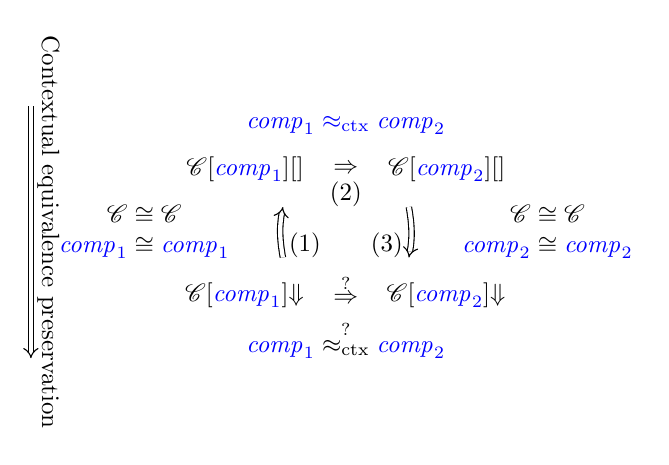
\begin{tikzpicture}[scale=0.8,every node/.style={scale=.9}]
    % \draw[help lines,yellow] (0,0) grid (10,7);
    \node at (5,4.7) { ${\src{\comp_1}\mathrel{\sconeq} \src{\comp_2}}$ };

    \node at (3.4,4) { ${\plug{\trg{\context}}{\src{\comp_1}} \sterm[]{\gc}{}}$ };
    \node at (5,4) { $\mathrel{\Rightarrow}$ };
    \node at (6.6,4) { ${\plug{\trg{\context}}{\src{\comp_2}} \sterm[]{\gc}{}}$ };

    \node at (4.35,2.8) { (1) };
    \node at (5,3.6) { (2) };
    \node at (5.65,2.8) { (3) };

    \draw[out=100,in=260,double,-implies,double equal sign distance] (4,2.6) to (4,3.4);

    \draw[out=280,in=80,double,-implies,double equal sign distance] (6,3.4) to (6,2.6);

    \node[align=center] at (8.2,3) { $ {\trg{\context}} \cong \trg{\context}$ \\
      $ {\src{\comp_2}} \cong {\src{\comp_2}}$};
    \node[align=center] at (1.8,3) { $ {\trg{\context}} \cong \trg{\context}$ \\
      $ {\src{\comp_1}} \cong {\src{\comp_1}}$};
    % \node at (9,2.7) { $e  {\src{C_1}} \cong \src{C_1}} : tau$ };
    % \node at (8.7,3.3) { $ {\trg{\context}} \cong \trg{\context} :{\emptyset},tau \ra e,{\cdots}$ };
    % \node at (.8,3) { $e  {\src{C_1}} \cong {\src{C_1}} : tau$ };

    \node at (3.4,2) { ${\plug{\trg{\context}}{\src{\comp_1}} \term[]{}}$ };
    \node at (5,2.1) { $\overset{?}{\Rightarrow}$ };
    \node at (6.6,2) { ${\plug{\trg{\context}}{\src{\comp_2}} \term[]{}}$ };

    \node at (5,1.3) { ${\src{\comp_1}}\mathrel{\overset{?}{\tconeq}}{\src{\comp_2}}$ };

    \draw[out=-90,in=90,double,-implies,double equal sign distance] (0,5) to node[sloped, yshift =.7em]{\Small Contextual equivalence preservation} (0,1);
  \end{tikzpicture}
  \caption{Proving one direction of fully abstract compilation (contextual equivalence preservation).}
  \label{fig:fa-proof-sketch}
\end{figure}


% \subsection{Proof sketch}
% \label{subsec:proof-sketch}
% \begin{proof}[Proof of Theorem~\ref{thm:full-abstraction}]
  % \item Consider first the upward arrow.
  %   Assume $\src{\var{comp}_1} \tconeq \src{\var{comp}_2}$.

  %   Take a $\src{\context}$ such that $\vdash \src{\context}$, take $\src{\ta[,i]}
  %   = \src{\dom(\var{comp}_i.\mscode)}$, $\gsigrets_i = \var{comp}_i.\sigrets$ and
  %   $\gsigcloss_i = \var{comp}_i.\sigcloss$, $\gc_i = (\ta[,i],\stkb_i,\gsigrets_i,\gsigcloss_i)$ and we will prove that
  %   $\src{\plug{\context}{\var{comp}_1} \sterm{\gc_1}} \Leftrightarrow
  %   \src{\plug{\context}{\var{comp}_2} \sterm{\gc_2}}$.

  %   By symmetry, we can assume w.l.o.g. that $\src{\plug{\context}{\var{comp}_1} \sterm{\gc_1}}$ and prove that $\src{\plug{\context}{\var{comp}_2} \sterm{\gc_2}}$.
  %   Note that this implies that $\src{\context}$ is a valid context for both $\src{\var{comp}_1}$ and $\src{\var{comp}_2}$.

  %   First, we show that also $\plug{\context}{\var{comp}_1} \trg{\term}$.
  %   Take $n$ the amount of steps in the termination of $\src{\plug{\context}{\var{comp}_1} \sterm{\gc_1}}$.
  %   It follows from Lemma~\ref{lem:ftlr-comps} that $\npair[n+1]{(\var{comp}_1,\var{comp}_1)} \in \lrcomp[\preceq,\gc_1](W_1)$ for some $W_1$ with $\dom(\pwfree) = \dom(\pwpriv) = \emptyset$.
  %   It also follows from the same Lemma~\ref{lem:ftlr-comps} that $\npair[n+1]{(\context,\context)} \in \lrcomp[\preceq,\gc_1](W_1')$ for some $W_1'$ that we can choose such that $W_1 \uplus W_1'$ is defined.
  %   Lemma~\ref{lem:compat-context-plug} then tells us that $\npair{(\plug{\context}{\var{comp}_1}, \plug{\context}{\var{comp}_1})} \in \lrec[\preceq,\gc_1](W_1\uplus W_1')$
  %   Together with $\src{\plug{\context}{\var{comp}_1} \sterm[n]{\gc_1}}$, Lemma~\ref{lem:adequacy} then tells us that $\plug{\context}{\var{comp}_1} \trg{\term}$.

  %   It follows from $\src{\var{comp}_1} \tconeq \src{\var{comp}_2}$ that also $\plug{\context}{\var{comp}_2} \trg{\term}$.

  %   It now remains to show that also $\src{\plug{\context}{\var{comp}_2} \sterm{\gc_2}}$.
  %   Take $n'$ the amount of steps in the termination of $\plug{\context}{\var{comp}_2} \trg{\term}$.
  %   It follows from Lemma~\ref{lem:ftlr-comps} that $\npair[n'+1]{(\var{comp}_2,\var{comp}_2)} \in \lrcomp[\succeq,\gc_2](W_2)$ for some $W_2$ with $\dom(\pwfree) = \dom(\pwpriv) = \emptyset$.
  %   It also follows from the same Lemma~\ref{lem:ftlr-comps} that $\npair[n'+1]{(\context,\context)} \in \lrcomp[\succeq,\gc_2](W_2')$ for some $W_2'$ that we can choose such that $W_2 \uplus W_2'$ is defined.
  %   Lemma~\ref{lem:compat-context-plug} then tells us that $\npair[n']{(\plug{\context}{\var{comp}_2}, \plug{\context}{\var{comp}_2})} \in \lrec[\succeq,\gc_2](W_2\uplus W_2')$
  %   Together with $\plug{\context}{\var{comp}_2} \trg{\term[n']}$, Lemma~\ref{lem:adequacy} then tells us that $\src{\plug{\context}{\var{comp}_2} \sterm{\gc_2}}$, concluding this direction of the proof.

%   First consider the right arrow:

%     Assume $\src{\var{comp}_1} \sconeq \src{\var{comp}_2}$. Take $\src{\ta[,i]} = \src{\dom(\var{comp}_i.\mscode)}$, $\gsigrets_i = \var{comp}_i.\sigrets$ and $\gsigcloss_i = \var{comp}_i.\sigcloss$, $\gc_i = (\ta[,i],\stkb_i,\gsigrets_i,\gsigcloss_i)$.
% %
%     Take a $\trg{\context}$ such that $\vdash \trg{\context}$ and we will prove that
%     $\trg{\plug{\context}{\var{comp}_1} \term} \Leftrightarrow
%     \trg{\plug{\context}{\var{comp}_2} \term}$.
% %
%     By symmetry, we can assume w.l.o.g. that $\trg{\plug{\context}{\var{comp}_1} \term}$ and prove that $\trg{\plug{\context}{\var{comp}_2} \term}$.
%     Note that this implies that $\trg{\context}$ is a valid context for both $\trg{\var{comp}_1}$ and $\trg{\var{comp}_2}$.
% %
%     First, we show that also $\plug{\context}{\var{comp}_1} \src{\sterm{\gc_1}}$.
%     Take $n$ the amount of steps in the termination of $\plug{\context}{\var{comp}_1} \trg{\term}$.
%     It follows from Lemma~\ref{lem:ftlr-comps} that $\npair[n+1]{(\var{comp}_1,\var{comp}_1)} \in \lrcomp[\succeq,\gc_1](W_1)$ for some $W_1$ with $\dom(\pwfree) = \dom(\pwpriv) = \emptyset$.
%     It also follows from the same Lemma~\ref{lem:ftlr-comps} that $\npair[n+1]{(\context,\context)} \in \lrcomp[\succeq,\gc_1](W_1')$ for some $W_1'$ that we can choose such that $W_1 \uplus W_1'$ is defined.
%     Lemma~\ref{lem:compat-context-plug} then tells us that $\npair{(\plug{\context}{\var{comp}_1}, \plug{\context}{\var{comp}_1})} \in \lrec[\succeq,\gc_1](W_1\uplus W_1')$
%     Together with $\plug{\context}{\var{comp}_1} \trg{\term[n]}$, Lemma~\ref{lem:adequacy} then tells us that $\plug{\context}{\var{comp}_1} \src{\sterm{\gc_1}}$.
% %
%     It follows from $\src{\var{comp}_1} \sconeq \src{\var{comp}_2}$ that also $\plug{\context}{\var{comp}_2} \src{\sterm{\gc_2}}$.
% %
%     It now remains to show that also $\plug{\context}{\var{comp}_2} \trg{\term}$.
%     Take $n'$ the amount of steps in the termination of $\plug{\context}{\var{comp}_2} \src{\sterm{\gc_2}}$.
%     It follows from Lemma~\ref{lem:ftlr-comps} that $\npair[n'+1]{(\var{comp}_2,\var{comp}_2)} \in \lrcomp[\preceq,\gc_2](W_2)$ for some $W_2$ with $\dom(\pwfree) = \dom(\pwpriv) = \emptyset$.
%     It also follows from the same Lemma~\ref{lem:ftlr-comps} that $\npair[n'+1]{(\context,\context)} \in \lrcomp[\preceq,\gc_2](W_2')$ for some $W_2'$ that we can choose such that $W_2 \uplus W_2'$ is defined.
%     Lemma~\ref{lem:compat-context-plug} then tells us that $\npair[n']{(\plug{\context}{\var{comp}_2}, \plug{\context}{\var{comp}_2})} \in \lrec[\preceq,\gc_2](W_2\uplus W_2')$
%     Together with $\plug{\context}{\var{comp}_2} \trg{\term[n']}$, Lemma~\ref{lem:adequacy} then tells us that $\plug{\context}{\var{comp}_2} \trg{\term}$, concluding the second direction of the proof.

%  The left arrow is proven in a similar manner.
% \end{proof}

%%% Local Variables:
%%% TeX-master: "paper"
%%% End:

\section{Discussion}
\label{sec:discussion}
% \begin{itemize}
% \item explain how fully abstract overlay semantics could form one pass of a verified secure compiler.
% \item Sharing stack references accross component boundaries is supported
% \item Other notions of well-bracketedness (specifically one would be to allow different stacks)
% \end{itemize}
\subsection{Full Abstraction}
% - Full abstraction proofs difficult
Our formulation of WBCF and LSE using a fully abstract overlay semantics has an important advantage with respect to others.
Imagine that you are implementing a fully abstract compiler for a high-level language, i.e.\ a secure compiler that enforces high-level abstractions when interacting with untrusted target-language components.
Such a compiler would need to perform many things and enforce other high-level properties than just WBCF and LSE.

If such a compiler uses the \stktokens{} calling convention, then the security proof should not have to reprove security of \stktokens{}.
Ideally, it should just combine security proofs for the compiler's other functionality with our results about \stktokens{}.
We want to point out that our formulation enables such reuse.
Specifically, the compiler could be factored into a part that targets \srccm{}, followed by our embedding into \trgcm{}.
If the authors of the secure compiler can prove full abstraction of the first part (relying on WBCF and LSE in \srccm{}) and they can also prove that this first part generates well-formed and reasonable components, then full abstraction of the whole compiler follows by our result and transitivity of fully abstract compilation.
Perhaps other reusable components of secure compilers could be formulated similarly using some form of fully abstract overlay semantics, to obtain similar reusability of their security proofs.

% When creating fully-abstract compilers between low-level machines, it is a big challenge to work with the exposed addresses.
% In particular, if the compilation changes the code size of a block of code, then it may be observable and prevent full-abstraction from being proven.
% We would argue that when a compilation reaches a phase where addresses are exposed, then the compilation should no longer change the code.
% This does, however, pose the challenge that there might quite a few abstractions in difference between the language where addresses are hidden to a machine where they are not.
% We propose that this challenge is solved by implementing these abstractions in a number of overlay semantics.
% By implementing them one by one, one can deal with one abstraction at a time reducing the complexity of each necessary full-abstraction proof.


% - Need to compile to a machine with enforcement mechanisms - capability machine an option
% - Full abstraction proofs modular, so other full abstraction proofs could target \srccm{} and thus have more abstractions to work with than if \trgcm{} was the target.

%\subsection{Sharing the stack}
% ?
\subsection{Practical Applicability}
We believe there are good arguments for practical applicability of \stktokens{}.
The strong security guarantees are proven in a way that is reusable as part of a bigger proof of compiler security.
Its costs are
\begin{itemize}
\item a constant and limited amount of checks on every boundary crossing.
\item possibly a small memory overhead because stack frames must be of non-zero length
\end{itemize}
The main caveat is that we rely on the assumption that capability machines like CHERI can be extended with linear capabilities in an efficient way.

Although this assumption can only be discharged by demonstrating an actual implementation with efficiency measurements, the following notes are based on private discussions with people from the CHERI team as well as our own thoughts on the matter.
As we understand it, the main problems to solve for adding linear capabilities to a capability machine like CHERI are related to the move semantics for instructions like \texttt{move}, \texttt{store} and \texttt{load}.
Processor optimizations like pipelining and out-of-order execution rely on being able to accurately predict the registers and memory that an instruction will write to and read from.
Our instructions are a bit clumsy from this point-of-view because, for example, \texttt{move} or \texttt{store} will zero the source register resp. memory location if the value being written is linear.
A solution for this problem could be to add separate instructions for moving, storing and loading linear registers at the cost of additional opcode space.
Adding splice and split will also consume some opcode space.

Another problem is caused by the move semantics for \texttt{load} in the presence of multiple hardware threads.
In this setting, zeroing out the source memory location must happen atomically to avoid race conditions where two hardware threads end up reading the same linear capability to their registers.
This means that a \texttt{load} of a linear capability should behave atomically, similar to a primitive compare-and-swap instruction.
This is in principle not a problem except that atomic instructions are significantly slower than a regular \texttt{load} (on the order of 10x slower or more).
When using \stktokens{}, loads of linear capabilities happen only when a thread has stored its return data capability on the stack and loads it back from there after a return.
Because the stack is a region of memory with very high thread affinity (no other hardware thread should access it, in principle), and which is accessed quite often, well-engineered caching could perhaps reduce the high overhead of atomic loads of linear capabilities.
% If such memory could be (mostly) kept exclusively locked in a cache close to the processor, the overhead of atomic loads in \stktokens{} might be significantly less than \texttt{load}'s worst case.
The processor could perhaps also (be told to) rely on the fact that race conditions should be impossible for loads from linear capabilities (which should in principle be non-aliased) and just use a non-atomic load in that case.

%%% Local Variables:
%%% TeX-master: "paper"
%%% End:

\section{Related Work}
In this section, we discuss related work on securely enforcing control flow correctness and/or local state encapsulation or the linear capabilities we use to do it.
We do not repeat the work we discussed in Section~\ref{sec:introduction}.

Capability machines originate with \citet{dennis_programming_1966} and we refer to \citet{levy_capability-based_1984} and \citet{watson_cheri_2015} for an overview of previous work.
The capability machine formalized in Section~\ref{sec:cap-mach-w-seal-and-lin} is modelled after CHERI~\citep{watson_cheri_2015,woodruff_cheri_2014}.
This is a recent, relatively mature capability machine which combines capabilities with a virtual memory approach in the interest of backwards compatibility and gradual adoption.
For simplicity, we have omitted features of CHERI that were not needed for \stktokens{} (e.g.\ local capabilities, virtual memory).

Plenty of other papers enforce well-bracketed control flow at a low level but most are restricted to preventing particular types of attacks and enforce only partial correctness of control flow.
This includes particularly the line of work on control-flow integrity~\citep{abadi_control-flow_2005}.
This technique prevents certain classes of attacks by sanitizing addresses before direct and indirect jumps based on static control graph information and a protected shadow stack.
Contrary to \stktokens{}, CFI can be implemented on commodity hardware rather than capability machines.
However, its attacker model is different, and its security goals are weaker.
They assume an attacker that is unable to execute code but can overwrite arbitrary data at any time during execution (to model buffer overflows).
In terms of security goals, the technique does not enforce local stack encapsulation.
Also, it only enforces a weak form of control flow correctness saying that jumps stay within the program's static control flow graph~\cite{Abadi2005Theory}.
Such a property ignores temporal properties and seems hard to use for reasoning.
There is also more and more evidence that these partial security properties are not enough to prevent realistic attacks in practice~\citep{Evans:2015:CJW:2810103.2813646,Carlini2015ControlFlowBending}.

More closely related to our work are papers that use separate per-component stacks, a trusted stack manager and some form of memory isolation to enforce control-flow correctness as part of a secure compilation result~\citep{patrignani_modular_2016,juglaret_beyond_2016}.
Our work differs from theirs in that we use a different low-level security primitive (a capability machine with local capabilities rather than a machine with a primitive notion of compartments), and we do not use per-component stacks or a trusted stack manager but a single shared stack and a decentralized calling convention based on linear capabilities.
Both prove a secure compilation result from a high-level language which clearly implies a general form of control-flow correctness, but that result is not separated from the results about other aspects of their compiler.

CheriBSD applies a similar approach with separate per-component stacks and a trusted stack manager on a capability machine~\cite{watson_cheri_2015}.
The authors use local capabilities to prevent components from accidentally leaking their stack pointer to other components, but there is no actual capability revocation in play.
They do not provide many details on this mechanism and it is, for example, not clear if and how they intend to deal with higher-order interfaces (C function pointers) or stack references shared across component boundaries. 

The fact that our full abstraction result only applies to reasonable components (see Section~\ref{sec:form-secur-with}) makes it related to full abstraction results for unsafe languages.
In their study of compartmentalization primitives, \Citet{juglaret_beyond_2016} discuss the property of Secure Compartmentalizing Compilation (SCC): a variant of full abstraction that applies to unsafe source languages.
Essentially, they modify standard full abstraction so that preservation and reflection of contextual equivalence are only guaranteed for components that are {\itshape fully defined}, which means essentially that they do not exhibit undefined behavior in any fully defined context.
In follow-up work, \citet{Abate:2018:GCG:3243734.3243745} extend this approach to scenarios where components only start to exhibit undefined behavior after a number of well-defined steps. 
If we see reasonable behavior as defined behavior, then our full abstraction result can be seen as an application of this same idea.
Our results do not apply to dynamic compromise scenarios because they are intended to be used in the verification of a secure compiler where these scenarios are not relevant.
\dominique{Perhaps worth pointing out that (I suspect that) our step-bounded reasonability and FTLR, actually does apply in dynamic compromise scenario's.
  The idea would be to use the theorem multiple times with different step bounds and a different boundary between trusted and untrusted code.
  More concretely, if a component A starts behaving non-reasonable after 10 steps, then first apply the FTLR with n = 9 and component A trusted.
  Then apply the FTLR again with n > 10 and component A no longer trusted.
  Then you get stronger well-bracketedness guarantees until n=9 and weaker ones after that.
  This is a step-bounded version of the idea explained in \cite{patrignani_modular_2016}.}

Local capabilities can be used to ensure well-bracketed control-flow and local-state encapsulation as demonstrated by \citet{skorstengaard_reasoning_2017}.
Recently, \citet{tsampas_2019} demonstrated that an extension of local capabilities with multiple linearly ordered colours can be used to enforce the life time of stack references.
Specifically, a stack reference should not be able to outlive the stack frame it points to.
If \stktokens{} was extended with stack references, then it would also enforce reference life times.
Specifically in order to return from a call, we must use the return token, i.e.\ the stack.
The stack is linear, so if there are references to it, aside from the stack capability itself, then we cannot have a complete return token.
This means that we have to splice all the stack references together with the stack capability to complete the return token in order to return.
\citet{tsampas_2019} allow (almost) normal references that can be stored in multiple places at the same time.
This means that their approach is more like C than what \stktokens{} has to offer.
As explained in Section~\ref{sec:introduction}, these approaches have the downside that they require stack clearing (including unused parts) on boundary crossings.

In addition to the already-mentioned work on linear capabilities, \citet{van_strydonck_linear_2019} have recently used them in a secure (fully abstract) compiler for a C-like language with separation logic contracts.
A form of linear capabilities was also used in the SAFE machine developed within the CRASH/SAFE project \citep{DBLP:conf/sp/AmorimDGHPST15,DBLP:journals/jcs/AmorimCDDHPPPT16}.
\citet{Abate:2018:GCG:3243734.3243745} used micro-policy enforced linear return capabilities to ensure a cross-component stack discipline.
Their linear capabilities were designed specifically to enforce the stack discipline but behave similarly to ours with the notable difference that their linear return pointers are destroyed in a jump.

There are other notions of secure compilation than full-abstraction~\citep{abadi_protection_1998}.
\citet{abate_2019} present an overview of trace-based secure compilation properties.
Full abstraction is only one, relatively weak, property in their hierarchy.
It would be interesting to investigate if our compiler, i.e.\ the embedding function from \srccm{} into \trgcm{}, also satisfies some of their other properties.
While our current result implies that we can prove contextual equivalences in \trgcm{} components using \stktokens{}, by proving them instead in the more well-behaved \srccm{} semantics, such stronger properties would imply that we can also prove robust preservation of other (hyper-)properties in a similar manner.
We expect that, in addition to full abstraction, our embedding also satisfies Robust Relational Hyperproperty Preservation (RrHP, the strongest property in the hierarchy of \citeauthor{abate_2019}) and that a large part of our current proof (the back-translation and the logical relation) could be reused to establish this.
However, to do this, we would first need to extend our semantics with some form of traces and we have not investigated how best to do this. 


% \begin{acks}                            %% acks environment is optional
%                                         %% contents suppressed with 'anonymous'
%   %% Commands \grantsponsor{<sponsorID>}{<name>}{<url>} and
%   %% \grantnum[<url>]{<sponsorID>}{<number>} should be used to
%   %% acknowledge financial support and will be used by metadata
%   %% extraction tools.
%   This material is based upon work supported by the
%   \grantsponsor{GS100000001}{National Science
%     Foundation}{http://dx.doi.org/10.13039/100000001} under Grant
%   No.~\grantnum{GS100000001}{nnnnnnn} and Grant
%   No.~\grantnum{GS100000001}{mmmmmmm}.  Any opinions, findings, and
%   conclusions or recommendations expressed in this material are those
%   of the author and do not necessarily reflect the views of the
%   National Science Foundation.
% \end{acks}

\begin{acks}
  This research was supported in part by the ModuRes Sapere Aude
  Advanced Grant from The Danish Council for Independent Research for
  the Natural Sciences (FNU) and by Cost Action CA15123 EUTypes.
  Dominique Devriese held a Postdoctoral Fellowship from the Research Foundation - Flanders (FWO) during most of this research.
\end{acks}

\bibliography{references}


%% Appendix
% \appendix
% \section{Appendix}

% Text of appendix \ldots

\clearpage
\appendix
%% Appendix
\appendix
\section{Appendix}
In this appendix, we give more precise formulations of lemmas that were mentioned in the paper, and the most important supporting definitions and lemmas.
The goal is to provide details that can help to understand in more detail what we discuss in the paper. 
Full details and proofs are not given here, but for those we refer to the technical appendix~\citep{technical_appendix}.

\subsection{Logical relation}
\label{app:logical-relation}
% Text of appendix \ldots
\textbf{$n$-subset simulation}
\begin{mathpar}
  \inferrule{(s,\phi_\pub,\phi) = (s',\phi_\pub',\phi') \\
    \forall \hat{W} \ldotp H \; (s) \; (\hat{W}) \nsubeq H' \; (s') \; (\hat{W}) }
  { (v,s,\phi_\pub,\phi,H) \nsubsim (v',s',\phi_\pub',\phi',H')}
\end{mathpar}
%
\textbf{Transition system relations}
\begin{align*}
   \Rels &= \{(\phi_\pub, \phi) \in \powerset{\States^2}\times \powerset{\States^2} \mid \phi_\pub, \phi \text{ is reflexive and transitive and } \phi_\pub \subseteq \phi \}
\end{align*}
%
\textbf{Erasure}
\begin{align*}
  \lfloor W \rfloor_S \defeq \lambda r \ldotp 
  \begin{cases}
    W(r) & W(r).v \in S\\
    \bot & \text{otherwise}
  \end{cases}
\end{align*}
%
\textbf{Active region projection}
\begin{align*}
  \activeReg{} & : \Worlds \fun 2^\RegionNames \\
  \activeReg{W} & \defeq \dom(\erase{W}{\perma,\temp})
\end{align*}
%
\textbf{Revoke temporary regions in a world}
\begin{align*}
  \revokeTemp{} & : \Worlds \fun \Worlds \\
  \revokeTemp{W} & \defeq \lambda r \ldotp 
                   \begin{cases}
                     \revoked            & \text{if }W(r) = (\temp,s,\phi_\pub,\phi,H) \\
                     W(r)                & \text{otherwise}
                   \end{cases}
\end{align*}
%
\textbf{Projection of regions based on locality}
\[
  \localityReg(\gl,W) \defeq 
  \begin{cases}
    \dom(\erase{W}{\perma ,\temp}) & \text{if } \gl = \local \\
    \dom(\erase{W}{\perma}) & \text{if } \gl = \glob
  \end{cases}
\]
%
\textbf{Address stratification}
\begin{align*}
&\iota = (v,s,\phi_\pub,\phi,H) \text{ is address-stratified iff }\\
&\qquad\begin{multlined}
  \forall s', \hat{W}, n, \ms, \ms' \ldotp \\
  \npair{\ms},\npair{\ms'} \in H~ s'~ \hat{W} \Rightarrow \\
  \dom(\ms) = \dom(\ms') \wedge \\
  \forall \addr \in
  \dom(\ms)\ldotp \npair{\ms\update{\addr}{\ms'(\addr)}} \in H~ s'~ \hat{W}
\end{multlined}
\end{align*}


\subsection{Complete ordered family of equivalences (c.o.f.e)}
\newcommand{\seq}[1]{\ensuremath{\left\{#1_n\right\}_{n=0}^{\infty}}}
\newcommand{\seqn}[1]{\ensuremath{\left(#1\right)_{n=0}^{\infty}}}
\newcommand{\NN}{\ensuremath{\mathbb{N}}}
\newcommand{\Ul}{\ensuremath{\mathcal{U}}}
\newcommand{\Later}{\ensuremath{\blacktriangleright}}
\newcommand{\op}[1]{\ensuremath{#1^{\text{op}}}}
\newcommand{\comp}{\circ}
\newcommand{\iso}{\cong}
\renewcommand{\hom}[3]{#1(#2,#3)}

\label{app:cofe}
This is an excerpt from \citet{Birkedal:tutorial-notes} about c.o.f.e.'s.
\begin{definition}[o.f.e.] An \emph{ordered family of equivalence} (o.f.e) is a
  set and a family of equivalences $\left(X, \left( \nequal \right)_{n=0}^\infty
  \right)$ that satisfy the following properties: 
  \begin{itemize}
  \item $\nequal[0]$ is the total relation on $X$
  \item $\forall n \ldotp \forall x,y \in X \ldotp x \nequal[n+1] y \Rightarrow
    x \nequal y$
  \item $\forall x,y \in X \ldotp (\forall n\ldotp x \nequal y) \Rightarrow x = y$
  \end{itemize}
  We say that an o.f.e. $\left(X, \seqn{\nequal[n]}\right)$ is \emph{inhabited} if there
  exists an element $x \in X$.
\end{definition}

If you are familiar with metric spaces observe that o.f.e.'s are but a different
presentation of bisected $1$-bounded ultrametric spaces.

\begin{definition}[Cauchy sequences and limits]
  \label{def:cauchy-sequence}
  Let $\left(X, \seqn{\nequal} \right)$ be an o.f.e. and $\seq{x}$ be a sequence of
  elements of $X$. Then $\seq{x}$ is a \emph{Cauchy sequence} if
  \begin{align*}
    \forall k \in \nats, \exists j \in \nats, \forall n \geq j, x_j \nequal[k] x_n
  \end{align*}
  or in words, the elements of the chain get arbitrarily close.

  An element $x \in X$ is the \emph{limit} of the sequence $\seq{x}$ if
  \begin{align*}
    \forall k \in \nats, \exists j \in \nats, \forall n \geq j, x \nequal[k] x_n.
  \end{align*}
  A sequence may or may not have a limit. If it has we say that the sequence
  \emph{converges}. The limit is necessarily unique in this case
  and we write $\lim_{n\to\infty}x_n$ for it.
\end{definition}

\begin{definition}[c.o.f.e.] A \emph{complete} ordered family of equivalences
  (c.o.f.e) is an o.f.e $\left(X, \left( \nequal \right)_{n=0}^\infty \right)$
  where all Cauchy sequences have a limit.  
\end{definition}

\begin{definition}
  \label{def:nonexpansive-contractive-ofe}
  Let $\left(X, \seqn{\nequal_{X}}\right)$ and $\left(Y, \seqn{\nequal_{Y}}\right)$ be
  two ordered families of equivalences and $f$ a function from the set $X$ to the set $Y$.
  The function $f$ is 
  \begin{itemize}
  \item \emph{non-expansive} if for any $x, x' \in X$, and any $n \in \nats$,
    \begin{align*}
      x \nequal_X x' \implies f(x) \nequal_Y f(x')
    \end{align*}
  \item \emph{contractive} if for any $x, x' \in X$, and any $n \in \nats$,
    \begin{align*}
      x \nequal_X x' \implies f(x) \nequal[n+1]_Y f(x')
    \end{align*}
  \end{itemize}
\end{definition}

\begin{theorem}[Banach's fixed point theorem]
  \label{thm:banach-fixed-point}
  Let $\left(X, \seqn{\nequal}\right)$ be a an inhabited c.o.f.e. and $f : X \to X$ a contractive
  function. Then $f$ has a unique fixed point.
\end{theorem}

\begin{definition}[The category $\Ul$]
  The category $\Ul$ of complete ordered families of equivalences has as objects complete
  ordered families of equivalences and as morphisms non-expansive functions.
\end{definition}

\begin{definition}
  \label{def:later-functor}
  The functor $\Later$ is a functor on $\Ul$ defined as
  \begin{align*}
    \Later\left(X, \seqn{\nequal}\right) &= \left(X,
          \seqn{\overset{n}{\equiv}}\right)\\
    \Later(f) &= f
  \end{align*}
  where $\overset{0}{\equiv}$ is the total relation and $x \overset{n+1}{\equiv} x'$
  iff $x \nequal x'$
\end{definition}

From now on, we often use the underlying set $X$ to denote a (complete) o.f.e. $\left(X,
  \seqn{\nequal}\right)$, leaving the family of equivalence
relations implicit.

\begin{definition}
 \label{def:nonexpansive-loc-contractive-functor}
 A functor $F : \op{\Ul} \times \Ul \to \Ul$ is \emph{locally non-expansive}  if for all
 objects $X$, $X'$, $Y$, and $Y'$ in $\Ul$ and
 $f, f' \in \hom{\Ul}{X}{X'}$ and $g, g' \in \hom{\Ul}{Y'}{Y}$ we have
 \begin{align*}
   f \overset{n}{=} f' \land g \overset{n}{=} g' \implies F(f, g) \overset{n}{=} F(f', g').
 \end{align*}

 It is \emph{locally contractive} if the stronger implication
 \begin{align*}
   f \overset{n}{=} f' \land g \overset{n}{=} g' \implies F(f, g) \overset{n+1}{=} F(f', g').
 \end{align*}
 holds. Note that the equalities are equalities on function spaces.
\end{definition}

\begin{proposition}
  \label{prop:loc-nonexp-loc-contr}
  If $F$ is a locally non-expansive functor then $\Later \comp F$ and $F \comp \left(\op{\Later}
  \times \Later\right)$ are locally contractive. Here, the functor $F \comp \left(\op{\Later} \times
  \Later\right)$ works as
  \begin{align*}
    (F \comp (\op{\Later} \times \Later))(X, Y) = F\left(\op{\Later}(X), \Later(Y)\right)
  \end{align*}
  on objects and analogously on morphisms and
  $\op{\Later} : \op{\Ul} \to \op{\Ul}$ is just $\Later$ working on $\op{\Ul}$ (i.e., its
  definition is the same).
\end{proposition}

\begin{definition}
 \label{def:fixed-point}
 A fixed point of a locally contractive functor $F$ is an object $X \in \Ul$, such that
 $F(X, X) \iso X$.
\end{definition}

The following is America and Rutten's fixed point theorem~\citep{America-Rutten:JCSS89}.
\begin{theorem}
 \label{thm:contr-functors-have-fixed-points}
 Every locally contractive functor $F$ such that $F(1, 1)$ is inhabited has a unique fixed
 point. The fixed point is unique among inhabited c.o.f.e.'s.
 If in addition $F(\emptyset, \emptyset)$ is inhabited then the fixed point of $F$ is unique.
\end{theorem}
In~\citet{BirkedalL:metric-enriched-journal} one can find a
category-theoretic generalization, which shows how to obtain fixed
points of locally contractive funtors on categories enriched in $\Ul$,
in particular on the category of preordered c.o.f.e.'s.  A preodered c.o.f.e. is
a c.o.f.e. equipped with a preorder that is closed under taking limits of
converging sequences.
The formulation in \emph{loc. cit.} also applies to solve
mutually recursive domain equations on preordered c.o.f.e.'s; see~\citet{bizjak:mutually-recursive-mcat}
for an explicit statement. That is the solution theorem we use to prove
Theorem~\ref{thm:world-existence}.



\subsection{Load instruction sufficiency lemma}
 \begin{lemma}[Conditions for store instruction are sufficient]
   \label{lem:conds-store-suff}
   If 
   \begin{itemize}
   \item $\ms = \ms' \uplus \ms_f$
   \item $\heapSat[\ms']{n}{W}$
   \item $((\perm,\gl),\start,\addrend,\addr) = c$
   \item $\npair{c}\in\stdvr(W)$
   \item $\writeAllowed{\perm}$
   \item $\withinBounds{\var{c}}$
   \item $\npair{\var{w}}\in\stdvr(W)$
   \item if $\var{w} = ((\_,\local),\_,\_,\_)$, then $\perm \in
     \{\rwlx,\readwritel \}$
   \end{itemize}
 
   then $\addr \in \dom(\ms')$ (i.e. $\ms\update{a}{w} =
   \ms'\update{a}{w}\uplus\ms_f$) and
   $\heapSat[{\ms'\update{\addr}{\var{w}}}]{n}{W}$
 \end{lemma}


\subsection{Macros}
\label{app:macros}
Implementation of the macros used in \texttt{scall}. Implementations of the
macros not presented here can be found in the technical
appendix~\citep{technical_appendix}.\\
\texttt{push $r$}
\begin{lstlisting}[xleftmargin=0.4cm]
  lea r_stk 1
  store r_stk r
\end{lstlisting}
\texttt{pop $r$}
\begin{lstlisting}[xleftmargin=0.4cm]
  load r r_stk
  minus r_t1 0 1
  lea r_stk r_t1
\end{lstlisting}
\texttt{rclear $r_1,\dots, r_n$}
\begin{lstlisting}[xleftmargin=0.4cm]
  move $r_1$ 0
  move $r_2$ 0
  $\dots$
  move $r_n$ 0
\end{lstlisting}
\texttt{mclear $r$}
\begin{lstlisting}[xleftmargin=0.4cm]
  move r_t $r$
  getb r_t1 r_t
  geta r_t2 r_t
  minus r_t2 r_t1 r_t2
  lea r_t r_t2
  gete r_t2
  minus r_t1 r_t2 r_t1
  plus r_t1 r_t1 1
  move r_t2 pc
  lea r_t2 $\var{off}_\var{end}$ 
  move r_t3 pc
  lea r_t3 $\var{off}_\var{iter}$
iter:
  jnz r_t2 r_t1
  store r_t 0
  lea r_t 1
  plus r_t1 r_t1 1
  jmp r_t3
end:
  move r_t 0
  move r_t1 0
  move r_t2 0
  move r_t3 0
\end{lstlisting}
Where $\var{off}_\var{end}$ and $\var{off}_\var{iter}$ are the offsets to the label \texttt{end} % 9
and \texttt{iter}, % 2
respectively.
\newline\newline
\texttt{call} $r(\bar{r}_{\var{args}},\bar{r}_{\var{priv}})$
\newline
The \texttt{call} macro constitutes a calling convention based on heap allocated activation records.
This alternative to \texttt{scall} is included to illustrate that the logical relation can be used to reason about other calling conventions.
In the following, $\bar{r}_{\var{args}}$ and $\bar{r}_{\var{priv}}$ are lists of registers. An overview of this call:
\begin{itemize}
\item Set up activation record
\item Create local enter capability for activation (protected return pointer)
\item Clear unused registers
\item Jump
\item Upon return: Run activation code
  \begin{itemize}
  \item Restore private registers
  \item Jump to return capability
  \end{itemize}
\end{itemize}
\begin{lstlisting}[xleftmargin=0.4cm]
  malloc r_t $size$ 
// store private state in activation record
  store r_t r_priv,1
  lea r_t 1
  store r_t r_priv,2
  lea r_t 1
  ...
  lea r_t 1
  store r_t r_priv,n
  lea r_t 1
// store old pc
  move r_t1 pc
  lea r_t1 $\var{off}_\var{end}$ 
  store r_t r_t1
  lea r_t1 1
// store activation record
  store r_t encode(i_1)
  lea r_t1 1
  ...
  lea r_t1 1  
  store r_t encode(i_m)
  lea r_t1 $k$ 
  restrict r_t1 encodePermPair(($\local$,e))
  move r_0 r_t1
// Clear unused registers
  rclear R // R = RegisterName - {r,pc,r_0,r_args}
  jmp r
end:
\end{lstlisting}
Where $\bar{r_{\var{priv}}} = r_{\var{priv},1}, \dots, r_{\var{priv},n}$, $size$ is the size of the activation record, $\var{off}_\var{end}$ is the offset to the \texttt{end} label, and $k$ is $m-1$, i.e. the offset to the first instruction of the activation code.\newline
The activation record. The instructions correspond to $i_1,\dots,i_m$ in the above.
\begin{lstlisting}[xleftmargin=0.4cm]
  move r_t pc
  getb r_t1 r_t
  geta r_t2 r_t
  minus r_t1 r_t1 r_t2
// load private state
  lea r_t r_t1
  load r_priv,1 r_t
  lea r_t 1
  load r_priv,2 r_t
  lea r_t 1
  ...
  lea r_t 1
  load r_priv,n r_t
  lea r_t 1
// load old pc
  load pc r_t
\end{lstlisting}

\subsection{Reasoning about programs definitions}
\label{app:programs-definitions}
\begin{definition}
  We say that $(\reg,\ms) \text{ is looking at } [i_0,\cdots,i_n] \text{ followed by } c_{\mathit{next}}$ 
  iff
  \begin{itemize}
  \item $\reg(\pcreg) = ((p,g),b,e,a)$
  \item $p = \rwx$, $p = \exec$, or $p = \rwlx$
  \item $a+n\leq e$, $b\leq a\leq e$
  \item $\ms(a+0,\cdots,a+n) = [i_0,\cdots,i_n]$
  \item $c_{\mathit{next}} = ((p,g),b,e,a+n+1)$
  \end{itemize}
\end{definition}

\begin{definition}
  We say that ``\linksto{(\reg,\ms)}{\var{key}}{j}{c}'' 
  iff
  \begin{itemize}
  \item $\reg(pc) = \stdcap$
  \item $\ms(\start) = ((\_,\_),\start_\link,\_,\_)$
  \item $\ms(\start_\link+j) = c$
  \end{itemize}
\end{definition}

\begin{definition}
  We say that $\reg \text{ points to stack with $\ms_\stk$ used and $\ms_{\mathit{unused}}$ unused}$
  iff
  \begin{itemize}
  \item $\reg(r_\stk) =((\rwlx,\local),b_\stk,e_\stk,a_\stk)$
  \item $\dom(\ms_{\mathit{unused}}) = [a_\stk+1,\cdots,e_\stk]$
  \item $\dom(\ms_\stk) = [b_\stk,\cdots,a_\stk]$ \lau{Maybe make it clear what happens when $\ms_\stk$ is empty}
  \item $b_\stk - 1\leq a_\stk$
  \end{itemize}
\end{definition}


 \subsection{Example correctness lemmas}
\begin{lemma}[Correctness lemma for \texttt{f1}, copy of Lemma~\ref{lem:correctness-f1}] \forcenewline
  \label{lem:correctness-f1-app}
  For all $n \in \nats$
  let
  \begin{align*}
    c_{\var{adv}} & \defeq ((\entry,\glob),\start_{\adv},\addrend_{\adv},\start_{\adv}+\olf) \\
    c_{f1} & \defeq ((\rwx,\glob),\mathtt{f1}-\olf,\mathtt{1f},\mathtt{f1}) \\
    c_\malloc & \defeq ((\entry,\glob),\start_\malloc,\addrend_\malloc,\start_\malloc+\olf) \\
    m & \defeq \hs_{f1} \uplus 
        \hs_\flag \uplus                
        \ms_{\var{link}} \uplus 
        \hs_\adv \uplus 
        \ms_{\malloc} \uplus 
        \hs_{\var{frame}} 
  \end{align*}
  and
  \begin{itemize}
  \item $c_\malloc$ satisfies the specification for malloc and $\iota_{\malloc,0}$ is the region from the specification.
  \end{itemize}
  where 
  \begin{align*}
    &\dom(\hs_{f1}) = [\mathtt{f1}-\olf,\mathtt{1f}] \\
    &\dom(\hs_\flag) = [\flag,\flag] \\
    &\dom(\ms_\link) = [\link,\link+1]\\
    &\dom(\hs_{\adv}) = [\start_\adv,\addrend_\adv] \\
    &\heapSat[\hs_{\malloc}]{n}{[0 \mapsto \iota_{\malloc,0}]}
  \end{align*}
  and
  \begin{itemize}
  \item $\ms_{f1}(\mathtt{f1}-\olf) = ((\readonly,\glob),\link,\link+1,\link)$, $\ms_{f1}(\mathtt{f1}-\olf+1) = ((\readwrite,\glob),\flag,\flag,\flag)$, the rest of $\hs_{f1}$ contains the code of $f1$.
  \item $\ms_\flag = [\flag \mapsto 0]$
  \item $\ms_{\var{link}} = [\var{link} \mapsto c_\malloc, \var{link} + 1 \mapsto c_\adv]$
  \item $\hs_\adv$ contains a global read-only capability for $\hs_\link$ on its first address. The remaining cells of the memory segment only contain instructions.
  \end{itemize}
  if 
  \[
    (\reg\update{\pcreg}{c_{f1}},m) \step[n] (\halted,m'),
  \]
  then
  \[
    m'(\flag) = 0
  \]  
\end{lemma}

\begin{lemma}[Correctness lemma for \texttt{f2}, detailed version of Lemma~\ref{lem:correctness-f2}]
  \label{lem:correctness-f2-app}
  let
  \begin{align*}
    c_{\var{adv}} & \defeq ((\entry,\glob),\start_{\adv},\addrend_{\adv},\start_{\adv}+\olf) \\
    c_{f2} & \defeq ((\rwx,\glob),\mathtt{f2}-\olf,\mathtt{2f},\mathtt{f2}) \\
    c_\malloc & \defeq ((\entry,\glob),\start_\malloc,\addrend_\malloc,\start_\malloc+\olf) \\
    c_{\var{stk}} & \defeq ((\rwlx,\local),\start_\stk,\addrend_\stk,\start_\stk-1) \\
    c_\link & \defeq ((\readonly,\glob),\link,\link+1,\link)\\
    \reg & \in \Regs \\
    m & \defeq \hs_{f2} \uplus 
        \hs_\flag \uplus                
        \ms_{\var{link}} \uplus 
        \hs_\adv \uplus 
        \ms_{\malloc} \uplus 
        \ms_{\var{stk}} \uplus
        \ms_{\var{frame}} 
  \end{align*}
  and
  \begin{itemize}
  \item $c_\malloc$ satisfies the specification for malloc and $\iota_{\malloc,0}$ is the region from the specification.
  \end{itemize}
  where 
  \begin{align*}
    &\dom(\hs_{f2}) = [\mathtt{f2}-\olf,\mathtt{2f}] \\
    &\dom(\hs_\flag) = [\flag,\flag] \\
    &\dom(\ms_\link) = [\link,\link+1]\\
    &\dom(\ms_\stk) = [\start_\stk, \addrend_\stk]\\
    &\dom(\hs_{\adv}) = [\start_\adv,\addrend_\adv] \\
    &\heapSat[\hs_{\malloc}]{n}{[0 \mapsto \iota_{\malloc,0}]} \qquad \text{ for all $n \in \nats$}
  \end{align*}
  and
  \begin{itemize}
  \item $\ms_{f2}(\mathtt{f2}-\olf) = ((\readonly,\glob),\link,\link+1,\link)$, $\ms_{f2}(\mathtt{f2}-\olf+1) = ((\readwrite,\glob),\flag,\flag,\flag)$, the rest of $\hs_{f2}$ contains the code of $f2$.
  \item $\ms_\flag = [\flag \mapsto 0]$
  \item $\ms_{\var{link}} = [\var{link} \mapsto c_\malloc, \var{link} + 1 \mapsto c_\adv]$
  \item $\hs_\adv(\start_\adv) = c_\link$ and $\forall \addr \in [\start_\adv+1,\addrend]\ldotp \ms_\adv(a) \in \ints$
  \end{itemize}
  if 
  \[
    (\reg\update{\pcreg}{c_{f2}}\update{r_\stk}{c_\stk},m) \step[n] (\halted,m'),
  \]
  then
  \[
    m'(\flag) = 0
  \]  
\end{lemma}
\begin{lemma}[Correctness lemma for \texttt{f3}, detailed version of Lemma~\ref{lem:correctness-f3}]
  \label{lem:correctness-f3-detailed}
  For all $n \in \nats$
  let
  \begin{align*}
    c_{\var{adv}} & \defeq ((\entry,\glob),\start_{\adv},\addrend_{\adv},\start_{\adv}+\olf) \\
    c_{f3} & \defeq ((\rwx,\glob),\mathtt{f3}-\olf,\mathtt{3f},\mathtt{f3}) \\
    c_{\var{stk}} & \defeq ((\rwlx,\local),\start_\stk,\addrend_\stk,\start_\stk-1) \\
    c_\malloc & \defeq ((\entry,\glob),\start_\malloc,\addrend_\malloc,\start_\malloc+\olf) \\
    c_\link & \defeq ((\readonly,\glob),\link,\link+1,\link) \\
    \reg & \in \Regs \\
    m & \defeq \hs_{f3} \uplus 
        \hs_\flag \uplus                
        \ms_{\var{link}} \uplus 
        \hs_\adv \uplus 
        \ms_{\malloc} \uplus 
        \ms_{\var{stk}} \uplus
        \ms_{\var{frame}} 
  \end{align*}
  and
  \begin{itemize}
  \item $c_\malloc$ satisfies the specification for malloc.
  \end{itemize}
  where 
  \begin{align*}
    &\dom(\hs_{f3}) = [\mathtt{f3}-\olf,\mathtt{3f}] \\
    &\dom(\hs_\flag) = [\flag,\flag] \\
    &\dom(\ms_\link) = [\link,\link+1]\\
    &\dom(\ms_\stk) = [\start_\stk, \addrend_\stk]\\
    &\dom(\hs_{\adv}) = [\start_\adv,\addrend_\adv] \\
    &\heapSat[\hs_{\malloc}]{n}{[0 \mapsto \iota_{\malloc,0}]}
  \end{align*}
  and
  \begin{itemize}
  \item $\ms_{f3}(\mathtt{f3}-\olf) = ((\readonly,\glob),\link,\link+1,\link)$, $\ms_{f3}(\mathtt{f3}-\olf+1) = ((\readwrite,\glob),\flag,\flag,\flag)$, the rest of $\hs_{f3}$ contains the code of $f3$.
  \item $\ms_\flag = [\flag \mapsto 0]$
  \item $\ms_{\var{link}} = [\var{link} \mapsto c_\malloc, \var{link} + 1 \mapsto c_\adv]$
  \item $\hs_\adv(\start_\adv) = c_\link$ and all other addresses of $\ms_\adv$ contain instructions.
  \end{itemize}
  if 
  \[
    (\reg\update{\pcreg}{c_{f3}}\update{r_\stk}{c_\stk},m) \step[n] (\halted,m'),
  \]
  then
  \[
    m'(\flag) = 0
  \]  
\end{lemma}

 
 \begin{lemma}[Correctness of $g1$, detailed version of Lemma~\ref{lem:correctness-g1}]
  \label{lem:correctness-g1-detailed}
  For all $n \in \nats$
  let
  \begin{align*}
    c_{\var{adv}} & \defeq ((\rwx,\glob),\start_{\adv},\addrend_{\adv},\start_{\adv}+\olf) \\
    c_{g1} & \defeq ((\entry,\glob),\mathtt{g1}-\olf,\mathtt{4f},\mathtt{g1}) \\
    c_\stk & \defeq ((\rwlx,\local),\start_\stk,\addrend_\stk,\start_\stk-1) \\
    c_\malloc & \defeq ((\entry,\glob),\start_\malloc,\addrend_\malloc,\start_\malloc+\olf) \\
    c_\link & \defeq ((\readonly,\glob),\link,\link,\link) \\
    m & \defeq \hs_{g1} \uplus 
        \ms_\flag \uplus                
        \ms_\link \uplus 
        \ms_\adv \uplus 
        \ms_\malloc \uplus 
        \ms_\stk \uplus
        \ms_{\var{frame}} 
  \end{align*}
  where 
  \begin{itemize}
  \item $c_\malloc$ satisfies the specification for malloc with $\iota_{\malloc,0}$
  \end{itemize}
  \begin{align*}
    &\dom(\hs_{g1}) = [\mathtt{g1}-\olf,\mathtt{4f}] \\
    &\dom(\hs_\flag) = [\flag,\flag] \\
    &\dom(\ms_\link) = [\link,\link]\\
    &\dom(\ms_\stk) = [\start_\stk, \addrend_\stk]\\
    &\dom(\hs_{\adv}) = [\start_\adv,\addrend_\adv] \\
    &\heapSat[\hs_{\malloc}]{n}{[0 \mapsto \iota_{\malloc,0}]}
  \end{align*}
  and
  \begin{itemize}
  \item $\ms_{g1}(\mathtt{g1}-\olf) = ((\readonly,\glob),\link,\link,\link)$, $\ms_{g1}(\mathtt{g1}-\olf+1) = ((\readwrite,\glob),\flag,\flag,\flag)$, the rest of $\hs_{g1}$ contains the code of $g1$ immediately followed by the code of $f4$.
  \item $\ms_\flag = [\flag \mapsto 0]$
  \item $\ms_{\var{link}} = [\link \mapsto c_\malloc]$
  \item $\hs_\adv(\start_\adv) = c_\link$ and all other addresses of $\ms_\adv$ contain instructions.
  \item $\forall a \in \dom(\ms_\stk) \ldotp \ms_\stk(a) = 0$ %This condition could be weakened to \memSat{\ms_\stk}{[\iota^\pwl(\dom(\ms_\stk))]}
  \end{itemize}
  if 
  \[
    (\reg_0\update{\pcreg}{c_\adv}\update{r_\stk}{c_\stk}\update{r_1}{c_{g1}},m) \step[n] (\halted,m'),
  \]
  then
  \[
    m'(\flag) = 0
  \]  
\end{lemma}


\subsection{Awkward example}
\label{app:awkward-example}
\textbf{The region for variable $x$} The region $\iota_x$, is the region omitted from the proof sketch for the awkward example.
\figurename~\ref{fig:x-reg} illustrates the transition system of $\iota_x$.
  \begin{figure}[tb]
    \centering
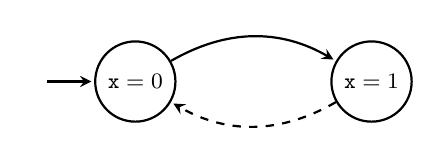
\begin{tikzpicture}[->,shorten >=1pt,auto,node distance=3cm,
  thick,main node/.style={circle,fill=white,draw,font=\sffamily\large},rect node/.style={rectangle,fill=blue!20,draw,font=\sffamily\large}]

  \node[main node] (n0) {\footnotesize $\texttt{x}=0$};
  \node (s) [left of=n0,xshift=1.75cm] {  };
  \node[main node] (n1) [right of=n0]  {\footnotesize $\texttt{x}=1$};
  \draw (s) edge[>=stealth] (n0);
  \draw (n0) edge[bend left,>=stealth] (n1);
  \draw (n1) edge[bend left,dashed,>=stealth] (n0);
  
\end{tikzpicture}
  \caption{Illustration of transition system in $\iota_x$. The dashed line is
    the private transition.}
  \label{fig:x-reg}
\end{figure}

\begin{definition}
  \label{def:iotax-region}
  \begin{align*}
    \iota_x   & = (\perm, 0, \phi_\pub, \phi, H_x) \\
    \phi_\pub & = \{(0,1)\}^* \\
    \phi      & = (1,0) \union \phi_\pub \\
    H_x \; s \; \hat{W} & = \{\npair{\ms} \mid \ms(x) = s \land n > 0 \} \union \{\npair[0]{\ms}\}
  \end{align*}
\end{definition}
\textbf{Static region} This static region only requires that the memory segment is the given one.
As it does not require safety, capabilities for this region cannot be gives to adversarial code.
\begin{align*}
  \iota^\sta (v,\ms) &= (v,1,=,=,H^\sta\;\ms)\\
  H^\sta \; \ms \; s \; \hat{W} = & \{\npair{\ms} \mid n > 0 \} \union \{\npair[0]{\ms'} \mid \ms' \in \Mems \}
\end{align*}
\textbf{Static safe region} Static region that also requires safety.
It is safe to give adversarial code read capabilities for this region.
\begin{align*}
  \iota^{\sta,u} (v,\ms) &= (v,1,=,=,H^{\sta,u}\;\ms)\\
  H^{\sta,u} \; \ms \; s \; \hat{W} = & \left\{\npair{\ms'} \middle|
    \begin{aligned}
      &\ms' = \ms \land{}\\
      &\forall \addr \in \dom(\ms) \ldotp\\
      & \quad \nonlocal{\ms(\addr)} \land{}\\
      & \quad \npair[n-1]{\ms(\addr)} \in \stdvr(\xi(\hat{W}))
    \end{aligned}
        \right\} \union \{\npair[0]{\ms'} \mid \ms' \in \Mems \}
\end{align*}



\end{document}
 